\documentclass[11pt]{book}

%% Copyright (C) 2014 Dorian Depriester
%% http://blog.dorian-depriester.fr
%%
%% This file may be distributed and/or modified under the conditions
%% of the LaTeX Project Public License, either version 1.3c of this
%% license or (at your option) any later version. The latest version
%% of this license is in:
%%
%%    http://www.latex-project.org/lppl.txt
%%
%% and version 1.3c or later is part of all distributions of LaTeX
%% version 2006/05/20 or later.
%%
%% This work has the LPPL maintenance status `maintained'.
%%
%% The Current Maintainer of this work is Dorian Depriester
%% <contact [at] dorian [-] depriester [dot] fr>.
%%
%% This is Preambule.tex for French PhD Thesis.



%%%%%%%%%%%%%%%%%%%%%%%%%%%%%%%%%%%%%%%%
%           Liste des packages         %
%%%%%%%%%%%%%%%%%%%%%%%%%%%%%%%%%%%%%%%%



%%%%%%%%%%%%%%%%%%%%%%%%%%%%%%%%%%%%%%%%%%%%%%%%%%%%%%%%%%%%%%%%%%%%%

%% Réglage des fontes et typo    
\usepackage[utf8]{inputenc}		% LaTeX, comprend les accents !
\usepackage[T1]{fontenc}
\usepackage{comment}

%\usepackage[square,sort&compress,sectionbib]{natbib}		% Doit être chargé avant babel
\usepackage{natbib}	
%\usepackage[frenchb]{babel}
\usepackage{lmodern}
\usepackage{ae,aecompl}										% Utilisation des fontes vectorielles modernes
\usepackage[upright]{fourier}



%%%%%%%%%%%%%%%%%%%%%%%%%%%%%%%%%%%%%%%%%%%%%%%%%%%%%%%%%%%%%%%%%%%%%
% Allure générale du document
\usepackage{enumerate}
\usepackage{enumitem}
\usepackage[section]{placeins}	% Place un FloatBarrier à chaque nouvelle section
\usepackage{epigraph}
\usepackage[font={small}]{caption}
\usepackage[francais,nohints]{minitoc}		% Mini table des matières, en français
	\setcounter{minitocdepth}{2}	% Mini-toc détaillées (sections/sous-sections)
\usepackage[notbib]{tocbibind}		% Ajoute les Tables	des Matières/Figures/Tableaux à la table des matières

%%%%%%%%%%%%%%%%%%%%%%%%%%%%%%%%%%%%%%%%%%%%%%%%%%%%%%%%%%%%%%%%%%%%%
%% Maths                         
\usepackage{amsmath}			% Permet de taper des formules mathématiques
\usepackage{amssymb}			% Permet d'utiliser des symboles mathématiques
\usepackage{amsfonts}			% Permet d'utiliser des polices mathématiques
\usepackage{nicefrac}			% Fractions 'inline'
\usepackage{bm}

%%%%%%%%%%%%%%%%%%%%%%%%%%%%%%%%%%%%%%%%%%%%%%%%%%%%%%%%%%%%%%%%%%%%%
%% Tableaux
\usepackage{multirow}
\usepackage{booktabs}
\usepackage{colortbl}
\usepackage{tabularx}
\usepackage{multirow}
\usepackage{threeparttable}
\usepackage{etoolbox}
	\appto\TPTnoteSettings{\footnotesize}


%%%%%%%%%%%%%%%%%%%%%%%%%%%%%%%%%%%%%%%%%%%%%%%%%%%%%%%%%%%%%%%%%%%%%
%% Eléments graphiques                    
\usepackage{graphicx}			% Permet l'inclusion d'images
\usepackage{subcaption}
\usepackage{pdfpages}
\usepackage{rotating}
\usepackage{pgfplots}
	\usepgfplotslibrary{groupplots}
\usepackage{tikz}
	\usetikzlibrary{backgrounds,automata}
	\pgfplotsset{width=7cm,compat=1.3}
	\tikzset{every picture/.style={execute at begin picture={
   		\shorthandoff{:;!?};}
	}}
	\pgfplotsset{every linear axis/.append style={
		/pgf/number format/.cd,
		use comma,
		1000 sep={\,},
	}}
\usepackage{eso-pic}
\usepackage{import}

%%%%%%%%%%%%%%%%%%%%%%%%%%%%%%%%%%%%%%%%%%%%%%%%%%%%%%%%%%%%%%%%%%%%%
%% Mise en forme du texte        
\usepackage{xspace}
\usepackage[load-configurations = abbreviations]{siunitx}
	\DeclareSIUnit{\MPa}{\mega\pascal}
	\DeclareSIUnit{\micron}{\micro\meter}
	\DeclareSIUnit{\tr}{tr}
	\DeclareSIPostPower\totheM{m}
	\sisetup{
	locale = FR,
	  inter-unit-separator=$\cdot$,
	  range-phrase=~\`{a}~,     	% Utilise le tiret court pour dire "de... à"
	  range-units=single,  		% Cache l'unité sur la première borne
	  }

\usepackage[version=3]{mhchem}	% Equations chimiques
\usepackage{textcomp}
\usepackage{array}
\usepackage{hyphenat}

%%%%%%%%%%%%%%%%%%%%%%%%%%%%%%%%%%%%%%%%%%%%%%%%%%%%%%%%%%%%%%%%%%%%%
%% Navigation dans le document
\usepackage[pdftex,pdfborder={0 0 0},
			colorlinks=true,
			linkcolor=blue,
			citecolor=red,
			pagebackref=true,
			]{hyperref}	% Créera automatiquement les liens internes au PDF
					% Doit être chargé en dernier (Sauf exceptions ci-dessous)
			

%%%%%%%%%%%%%%%%%%%%%%%%%%%%%%%%%%%%%%%%%%%%%%%%%%%%%%%%%%%%%%%%%%%%%
%% Packages qui doivent être chargés APRES hyperref	             
\usepackage[top=2.5cm, bottom=2cm, left=3cm, right=2.5cm,
			headheight=15pt]{geometry}

\usepackage{fancyhdr}			% Entête et pieds de page. Doit être placé APRES geometry
	\pagestyle{fancy}		% Indique que le style de la page sera justement fancy
	\lfoot[\thepage]{} 		% gauche du pied de page
	\cfoot{} 			% milieu du pied de page
	\rfoot[]{\thepage} 		% droite du pied de page
	\fancyhead[RO, LE] {}	
			% Liste des packages et de leurs options
%%%%%%%%%%%%%%%%%%%%%%%%%%%%%%%%%%%%%%%%
%           Commandes perso            %
%%%%%%%%%%%%%%%%%%%%%%%%%%%%%%%%%%%%%%%%

\newcommand{\alp}{\texorpdfstring{\ensuremath{\upalpha}\xspace}{alpha }}
\newcommand{\bet}{\texorpdfstring{\ensuremath{\upbeta}\xspace}{b\'{e}ta }}
\newcommand{\alpbet}{\texorpdfstring{\ensuremath{\upalpha-\upbeta}\xspace}{alpha-b\'{e}ta}}
\newcommand{\alpt}{\ensuremath{\alpha_2}\xspace}
\newcommand{\strt}{\gls{strt}\xspace}


% Tenseur des déformation cylindrique
\newcommand{\epsrr}{\ensuremath{\varepsilon_{rr}}\xspace}
\newcommand{\epstt}{\ensuremath{\varepsilon_{\theta\theta}}\xspace}
\newcommand{\epszz}{\ensuremath{\varepsilon_{zz}}\xspace}
\newcommand{\epsrt}{\ensuremath{\varepsilon_{r\theta}}\xspace}
\newcommand{\epstz}{\ensuremath{\varepsilon_{\theta z}}\xspace}
\newcommand{\epszr}{\ensuremath{\varepsilon_{zr}}\xspace}

\newcommand{\matlab}{\textsc{Matlab}\texttrademark\xspace}



%% Figures centrées, et en position 'here, top, bottom or page'
\newenvironment{figureth}{%
		\begin{figure}[htbp]
			\centering
	}{
		\end{figure}
		}
		
		
%% Tableaux centrés, et en position 'here, top, bottom or page'
\newenvironment{tableth}{%
		\begin{table}[htbp]
			\centering
			%\rowcolors{1}{coleurtableau}{coleurtableau}
	}{
		\end{table}
		}

%% Sous-figures centrées, en position 'top'		
\newenvironment{subfigureth}[1]{%
	\begin{subfigure}[t]{#1}
	\centering
}{
	\end{subfigure}
}

\newcommand{\citationChap}[2]{%
	\epigraph{\og \textit{#1} \fg{}}{#2}
}

%% On commence par une page impaire quand on change le style de numérotation de pages 
\let\oldpagenumbering\pagenumbering
\renewcommand{\pagenumbering}[1]{%
	\cleardoublepage
	\oldpagenumbering{#1}
}
	% Commandes et environnements perso
%% Copyright (C) 2014 Dorian Depriester
%% http://blog.dorian-depriester.fr
%%
%% This file may be distributed and/or modified under the conditions
%% of the LaTeX Project Public License, either version 1.3c of this
%% license or (at your option) any later version. The latest version
%% of this license is in:
%%
%%    http://www.latex-project.org/lppl.txt
%%
%% and version 1.3c or later is part of all distributions of LaTeX
%% version 2006/05/20 or later.
%%
%% This work has the LPPL maintenance status `maintained'.
%%
%% The Current Maintainer of this work is Dorian Depriester
%% <contact [at] dorian [-] depriester [dot] fr>.
%%
%% This is PageDeGarde.tex for French PhD Thesis.

%%%%%%%%%%%%%%%%%%%%%%%%%%%%%%%%%%%%%%%%%%
%           Page de Garde		         %
%%%%%%%%%%%%%%%%%%%%%%%%%%%%%%%%%%%%%%%%%%

\makeatletter
\def\@ecole{école}
\newcommand{\ecole}[1]{
  \def\@ecole{#1}
}

\def\@specialite{Spécialité}
\newcommand{\specialite}[1]{
  \def\@specialite{#1}
}

\def\@directeur{directeur}
\newcommand{\directeur}[1]{
  \def\@directeur{#1}
}

\def\@encadrant{encadrant}
\newcommand{\encadrant}[1]{
  \def\@encadrant{#1}
}
\def\@jurya{}{}{}
\newcommand{\jurya}[3]{
  \def\@jurya{#1,	& #2	& #3\\}
}
\def\@juryb{}{}{}
\newcommand{\juryb}[3]{
  \def\@juryb{#1,	& #2	& #3\\}
}
\def\@juryc{}{}{}
\newcommand{\juryc}[3]{
  \def\@juryc{#1,	& #2	& #3\\}
}
\def\@juryd{}{}{}
\newcommand{\juryd}[3]{
  \def\@juryd{#1,	& #2	& #3\\}
}
\def\@jurye{}{}{}
\newcommand{\jurye}[3]{
  \def\@jurye{#1,	& #2	& #3\\}
}
\def\@juryf{}{}{}
\newcommand{\juryf}[3]{
  \def\@juryf{#1,	& #2	& #3\\}
}
\def\@juryg{}{}{}
\newcommand{\juryg}[3]{
  \def\@juryg{#1,	& #2	& #3\\}
}
\def\@juryh{}{}{}
\newcommand{\juryh}[3]{
  \def\@juryh{#1,	& #2	& #3\\}
}
\def\@juryi{}{}{}
\newcommand{\juryi}[3]{
  \def\@juryi{#1,	& #2	& #3\\}
}
\makeatother

\newcommand\BackgroundPic{%
	\put(0,0){%
		\parbox[b][\paperheight]{\paperwidth}{%
			
\includegraphics[height=0.45\paperheight]{Bordure.png}%
			\vfill
		}
	}
}
\newcommand\EtiquetteThese{%
	\put(0,0){%
		\parbox[t][\paperheight]{\paperwidth}{%
			\hfill
			\colorbox{blue}{		
				\begin{minipage}[b]{3em}
					\centering\Huge\textcolor{white}{T\\H\\E\\S\\E\\}
					\vspace{0.2cm}
				\end{minipage}
			}
		}
	}
}

\makeatletter
\newcommand{\pagedegarde}{
\newgeometry{top=2.5cm, bottom=2cm, left=2cm, right=1cm}
\AddToShipoutPicture*{\BackgroundPic}
\AddToShipoutPicture*{\EtiquetteThese}
  \begin{titlepage}
  \centering
      
\includegraphics[width=0.4\textwidth]{ParisTech-Institute.pdf}
      \hfill
      
\includegraphics[width=0.2\textwidth]{Mines.pdf}\\
    \vspace{1cm}
      {\Large \'{E}cole doctorale \no 364 : Sciences Fondamentales et Appliquées}\\
    \vspace{1cm}
      {\huge 
      	{\bfseries Doctorat ParisTech}\\
    \vspace{0.5cm}
      	TH\`{E}SE}\\
    \vspace{1cm}
   		{\bfseries pour obtenir le grade de docteur délivré par}\\
    \vspace{1cm}
    	{\huge\bfseries \@ecole}\\
    \vspace{0.5cm}
    	{\Large{\bfseries Spécialité doctorale ``\@specialite''}}\\
    \vspace{2cm}
    	\textit{présentée et soutenue publiquement par}\\
    \vspace{0.5cm}
    	{\Large {\bfseries \@author}} \\
    \vspace{0.5cm}
    	le \@date \\
    \vfill
       {\LARGE \color[rgb]{0,0,1} \bfseries{\@title}} \\
    \vfill
        Directeur de thèse : {\bfseries \@directeur}\\
        Co-encadrant de thèse : {\bfseries \@encadrant}\\
    \vfill
	\begin{tabular}{>{\bfseries}llr}
		\large Jury\\
		\@jurya
		\@juryb
		\@juryc
		\@juryd
		\@jurye
		\@juryf
		\@juryg
		\@juryh
		\@juryi
	\end{tabular}
	\vfill
	
	\textbf{MINES ParisTech\\
	Centre de Mise Forme des Mat\'{e}riaux (CEMEF)}\\
	UMR CNRS 7635, F-06904 Sophia Antipolis, France
  \end{titlepage}




\restoregeometry  
  
  
}
\makeatother


%%% Commandes personnalisées  %%%
\newcommand{\nn}{\nonumber \\} % newline sans nombre dans align
\newcommand{\mC}{\mathcal{C}} %pour les fonctions de corrélation
\newcommand{\bx}{{\bf x}} %pour les vecteurs en gras
\newcommand{\by}{{\bf y}} %pour les vecteurs en gras
\newcommand{\bq}{{\bf q}}
\newcommand{\bk}{{\bf k}}
\newcommand{\br}{{\bf r}}
\newcommand{\bv}{{\bf v}}
\DeclareMathOperator{\sgn}{sgn}
% Les > et < se comportent normalement si c'est pour supérieur ou inférieur, sinon se comportent comme \langle
\mathchardef\less=\mathcode`<
\mathchardef\greater=\mathcode`>
\DeclareMathDelimiter{<}{\mathopen}{symbols}{"68}{largesymbols}{"0A}
\DeclareMathDelimiter{>}{\mathclose}{symbols}{"69}{largesymbols}{"0B}

%% Ne pas casser les équations inline $ $ 
\relpenalty=5000
\binoppenalty=5000


% Infos de la page de garde
\author{Paul Gersberg}
\title{Confinement and driving effects on continuous and discrete model interfaces}
\specialite{Laser, Matière, Nanosciences}
\directeur{David S. Dean}
\encadrant{Peter C.W. Holdsworth}
\date{20 juillet 2020}
\jurya{Steve Bramwell, Unversity College London}{Professeur}{Rapporteur}
\juryb{Jorge Kurchan, ENS, Paris}{Directeur de recherche}{Rapporteur}
\juryc{Pierre Pujol, Université Paul Sabatier, Toulouse }{Professeur}{Examinateur}
\juryd{Jérôme Cayssol, LOMA}{Professeur}{Examinateur}
\ecole{Université de Bordeaux}

% Méta-données du PDF
\hypersetup{
    pdfauthor={Dorian Depriester},
    pdfsubject={Manuscrit de thèse de doctorat},
    pdftitle={Fluotournage à froid de tubes en TA6V},
    pdfkeywords={Fluotournage, déformation plastique, titane, TA6V}
}

%%%%%%% Début du document %%%%%
\begin{document}
%\bibliographystyle{unrst}

% Préambule
	\pagenumbering{roman}
	\pagedegarde

	\cleardoublepage
{\bf Effets d'écoulements et de confinement dans les modèles discrets et continus d'interfaces} \\

Cette thèse examine les propriétés de l'interface entre deux phases dans un système avec des phases séparées. Nous regardons comment les effets de taille finis modifient les propriétés statistiques de ces interfaces, en particulier comment la dépendance de l'énergie libre par rapport à la taille du système donne lieu à des interactions de Casimir critique à longue portée proche du point critique.
Souvent, les interfaces sont décrites par des modèles simplifiés ou coarse-grained dont les seuls degrés de liberté sont les hauteurs de l'interface. Nous rappelons comment les propriétés statiques et dynamiques de ces interfaces sont retrouvées à partir de modèles microscopiques de spins et de théorie statistique des champs.
Nous étudions ensuite les effets de taille finie pour les interfaces continues comme le modèle Edwards-Wilkinson ou discrètes comme le modèle Solid-On-Solid, et discutons leur pertinence dans le cadre de l'effet Casimir critique.

Dans la seconde partie de la thèse, nous examinons des modèles d'interfaces sous écoulement qui possède des états stationnaires hors-équilibres. Nous développons 
ces équations dans le cadre du modèle C d'une interface, qui a un état stationnaire hors-équilibre lorsque soumis à un écoulement uniforme. L'état stationnaire hors-équilibre résultant exhibe des propriétés retrouvées dans les expériences sur des colloïdes sous cisaillement, notamment la suppression des fluctuations de la hauteur de l'interface et une augmentation de la longueur de corrélation des fluctuations. 
Finalement, nous proposons un nouveau modèle pour des interfaces uni-dimensionnelles qui est une modification du modèle Solid-on-Solid qui contient un terme supplémentaire d'entropie, ce qui le rend plus approprié pour l'étude de la diffusion et du cisaillement.
\\ \\
{\bf Keywords : } Modèles d'interface, Théorie d'ordonnancement des phases, Modèle d'Ising, Modèle Solid-On-Solid, Force de Casimir, Écoulements stationnaires hors-équilibre



{\bf Confinement and driving effects on continuous and discrete model interfaces}\\
This thesis examines the properties  of the interface between two phases in  phase separated systems. We are interested 
in how finite size effects modify the statistical properties of these interfaces, in particular  the dependence of the free energy on the system size 
gives rise to long range critical Casimir forces close to the critical point. Often the interfaces in phase separated systems are
described by simplified or coarse grained models whose only degrees of freedom are the interface height. We review how the statics and dynamics of
these  interface models can be derived from microscopic spin models and statistical field theories. We then examine finite size effects for 
continuous interface models such as the Edwards Wilkinson model and discrete models such as the Solid-On-Solid model  and discuss their 
relevance to the critical Casimir effect. In the second part of the thesis we examine models of driven interfaces which have nonequilibrium steady states. 
We develop a model C type model of an interface which shows a nonequlibrium steady
state even with constant driving. The resulting nonequlibrium steady state shows properties seen in experiments on sheared colloidal systems,
notably the suppression of height fluctuations but   a increase in the  correlation length of the fluctuations. Finally we propose a new model for
one dimensional interfaces which is a modification of  the solid-on-solid model and which contains extra entropic terms which make it more
appropriate to study diffusive dynamics and driving.
\\ \\
{\bf Keywords : }  Interface models, phase ordering dynamics, Ising model, Solid-On-Solid model, Casimir force, driven nonequilibrium steady states

\cleardoublepage
\chapter*{Résumé en français} 

La majorité des systèmes statistiques peuvent être décrits par un paramètre d'ordre, comme la magnétisation moyenne dans les systèmes magnétiques, la densité dans un fluide ou l'orientation moyenne des polymères dans les cristaux liquides. Les propriétés statiques et dynamiques de tels systèmes est bien décrite par la théorie statistique des champs. Dans cette théorie, le champ $\phi$ est soumis à un hamiltonien $H(\phi)$, et ses propriétés peuvent être dérivée de la fonction de partition $Z$.
Lorsque ces systèmes possèdent une transition de phase au point critique, il y a une discontinuité de l'énergie libre due à la modification des micro-configurations possibles. 
Dans les systèmes magnétiques, on passe ainsi d'une magnétisation nulle à une magnétisation finie, les liquides qui étaient auparavant mélangés se séparent, et les polymères adoptent une direction moyenne commune. Dans la phase ordonnée on retrouve alors des composantes connexes où la valeur de $\phi$ est quasi-constante. Entre ces composantes connexes se situe l'interface entre les phases. 
Dans cette thèse, nous nous intéressons particulièrement aux propriétés statiques et dynamiques des interfaces dans des modèles continus et discrets avec des contraintes telles que le confinement ou le cisaillement. 

\section*{Description d'une interface} 

La première partie de cette thèse est consacrée à la description des interfaces à partir de la théorie statistique des champs. L'utilisant un champ externe $\phi^4$ dans l'Hamiltonien induit une séparation de phase en dessous de la température critique, ce qui donne une interface dont le profil peut-être calculé grâce aux équations dynamiques du modèle A dans le cas stationnaire. L'énergie libre associée à cette interface est directement reliée à la tension superficielle $\sigma$ par la relation de Cahn-Hilliard.
Depuis les équations de théorie statistique des champs, en considérant une interface d'épaisseur nulle, on retrouve les équations d'Edwards-Wilkinson pour le modèle A et le modèle B. La réduction du nombre de degrés de liberté par cette transformation d'un volume en surface permet leur étude grâce à des intégrales de chemin, qui seront détaillées plus tard.

Ensuite nous expliquons le modèle le plus simple sur réseaux, le modèle d'Ising, qui décrit un réseau orthogonal de spins avec une interaction uniquement entre les plus proches voisins et un champ externe. Ce modèle, où chaque site du réseau prend la valeur $\sigma_1 = \pm1$, permet également de modéliser un système de gaz sur réseau ou de liquides binaires en faisant un changement de variable sur $\sigma_i$. En appliquant la même approximation d'interface d'épaisseur nulle que précédemment, on trouve cette fois-ci le modèle Solid-On-Solid. La fonction de partition SOS a l'avantage d'être diagonalisée grâce à la matrice de transfert, dont le formalisme est développé. Dans la limite thermodynamique, seul l'état fondamental (qui possède la plus grande valeur propre de la matrice de transfert) est nécessaire pour obtenir toutes les observables du système. 

Dans ce premier chapitre, une grande importance est également donnée quant à la différence entre les différents ensembles statistiques. La complexité de l'ensemble canonique provient de la contrainte sur la hauteur totale de l'interface qui ne peut être intégrée au formalisme des matrices de transfert. Pour étudier ces différences, il faut donc utiliser des méthodes numériques. Dans l'ensemble canonique, il est également possible d'introduire des états stationnaires hors-équilibre grâce à l'advection d'un champ de vitesse, que nous introduisons ici mais discuterons dans le dernier chapitre.


\section*{Méthodes numériques}

Dans ce chapitre, nous développons le fonctionnement des simulations de Monte Carlo Métropolis, qui permettent d'explorer l'espace des configurations et ainsi obtenir les valeurs moyennes d'observables. Ces méthodes sont particulièrement adaptées aux systèmes sur réseau comme le modèle d'Ising ou Solid-On-Solid, et on utilise alors l'algorithme de Glauber ou de Kawasaki selon l'ensemble thermodynamique dans lequel on se place. 

Néanmoins, l'énergie libre n'est pas une valeur mesurable directement dans les simulations de Monte Carlo, et il faut alors utiliser des méthodes indirectes. La méthode de Vasilyev consiste à découpler progressivement une rangée du système afin d'obtenir la dérivée de l'énergie libre par rapport à la taille du système. Cette méthode ne fonctionnant pas dans le cas du modèle SOS à cause de l'absence de terme de volume dans son hamiltonien, on utilise alors la méthode Lopes-Jacquin-Holdsworth, qui a été développée dans le cas d'un champ magnétique uniforme. Puisque l'intensité du champ magnétique est la valeur conjuguée de la magnétisation totale, on calcule alors l'intégrale de la magnétisation entre deux intensités afin d'obtenir la différence entre l'énergie libre des deux systèmes. Puisque cette méthode utilise la magnétisation, elle ne peut donc pas être utilisée lorsque le paramètre d'ordre est conservé, ce qui nous mène à une conclusion : il n'existe pas de méthode pour la mesure de l'énergie libre dans des simulations numériques de Kawasaki pour le modèle SOS.

Le chapitre se termine avec une petite liste d'astuces à connaître pour celui qui désirerait reproduire mes résultats numériques, principalement sur l'optimisation du code et la parallélisation.

\section*{Interfaces à l'équilibre et effets de taille finie}

Lorsque la longueur de corrélation est du même ordre de grandeur que la taille du système, la contrainte imposée sur les modes mous de fluctuations ajoute une partie singulière à l'énergie libre. Cette dépendance de l'énergie libre en fonction de la taille du système implique une force thermodynamique qui s'appelle force de Casimir dans le cas des fluctuations du champ électromagnétique entre deux plaques diélectriques parfaitement conductrices, ou effet Casimir critique dans les systèmes critiques. Après avoir exposé ces deux effets grâce à la mécanique quantique et le groupe de renormalisation, nous étudions cette force de confinement dans le cas des interfaces confinées. 

En utilisant le formalisme de Matsubara pour l'équation du propagateur de l'hamiltonien dans le cas d'une interface continue soumise à champ externe, nous explicitons la distribution de probabilité de l'interface, l'énergie libre, la fonction de corrélation à deux points et la longueur de corrélation en fonction de l'énergie de l'état fondamental et du premier état excité. En appliquant ce formalisme à une interface libre et confinée, on retrouve des résultats connus sur la force thermodynamique. Dans le cas où cette interface ne possède pas de tension superficielle (comme c'est le cas dans les systèmes critiques), la correction de taille finie à la tension superficielle proposée par Privman nous permet de retrouver quantitativement le même comportement que pour la force de Casimir critique. Nous utilisons également ce formalisme dans le cas où l'interface est confinée à cause d'une pression afin de trouver la hauteur de moyenne de l'interface et sa variance.

Puisque la méthode Lopes-Jacquin-Holdsworth de calcul de l'énergie libre dans les simulations de Monte Carlo n'est pas utilisable dans la dynamique de Kawasaki et que la méthode de Vasilyev ne l'est pas non plus pour les modèles SOS, nous généralisons la méthode LJH pour des champs externes non-uniformes, ce qui permet l'intégration sur une magnétisation généralisée qui n'est plus conservée dans une dynamique de Kawasaki. Nous montrons que cette généralisation est en accord avec la matrice de transfert SOS, et observons le même comportement de l'énergie libre pour les dynamiques de Glauber et de Kawasaki.

Ce troisième chapitre s'achève par la diagonalisation exacte de la matrice de transfert du modèle SOS en absence de potentiel externe, généralisant ainsi les résultats de Privman, et nous étudions les limites à faible et haute température ainsi que dans la limite thermodynamique.

\section*{Le modèle Particles-Over-Particles}

Le modèle SOS est un modèle d'interface provenant de l'approximation à basse température du modèle d'Ising. Nous développons dans ce quatrième chapitre un nouveau modèle : le modèle POP. Ce nouveau modèle prend en compte le terme d'entropie associé au modèle d'Ising et qui se retrouve aisément lorsque l'on fait des simulations numériques sur Ising, mais qui font défaut dans SOS. Ce terme d'entropie apparaît lorsque l'on considère non plus juste la hauteur de l'interface (comme dans SOS), mais également le nombre de particules en dessous. En labellisant ainsi les particules, il devient possible de créer des modèles avec $M$ types différents de particules, chacune étant régie par un coefficient cinétique ou un coefficient de diffusion dans le cas où elles appartiennent à des ensembles thermodynamiques différents. Nous finissons le chapitre en montrant comment procéder aux simulations numériques dans ce modèle, que nous comparons à la matrice de transfert. 

\section*{Interfaces stationnaires hors-équilibre} 

Lorsqu'une interface est advectée par un champ de vitesse, sa largeur et sa longueur de corrélation sont modifiées. Le cinquième et dernier chapitre s'intéresse à un écoulement uniforme et constant. 

À cause de l'invariance galiléenne de translation dans le référentiel de l'écoulement, l'équation dynamique du modèle B reste inchangée. Le cas d'un champ soumis au modèle B et couplé à un autre champ soumis au modèle A (afin de briser l'invariance galiléenne) a été l'objet d'un article publié dans {\bf Journal of Statistical Mechanics: Theory and Experiment} en mars 2020, et la première partie de ce chapitre est une reproduction de l'article original. À partir des équations couplées donnant le modèle C, on trouve une relation fermée pour la dynamique d'une interface soumis à un écoulement uniforme et constant dans l'espace de Fourrier. Cette méthode donne est valable pour une théorie gaussienne de l'interface, et l'écoulement introduit de la nouvelle physique, principalement que la tension de surface effective du système ainsi que la longueur de corrélation des fluctuations de l'interface sont augmentées. Ces résultats sont en accord qualitative avec les expériences de cisaillement sur les colloïdes. Tandis que la théorie sur les grandes longueurs d'onde que nous trouvons se comporte comme celles d'une onde capillaire, nous trouvons les ordres suivants qui sont générés par le spectre de la hauteur des fluctuations. De plus, nous montrons comment ce modèle permet de décrire l'interface entre deux phases de colloïdes ayant une activité différente en jouant sur la température de chaque phase, ce qui nous donne de nouveaux résultats que nous ne pourrions trouver dans le cas à l'équilibre.

Nous passons ensuite aux modèles sur réseau, et étudions la dépendance de la variance des hauteurs et de la tension superficielle de l'interface SOS en fonction de l'écoulement. Nous trouvons que contrairement au modèle C, l'écoulement a tendance augmenter la largeur de l'interface, de la même manière que le vent à la surface de l'océan génère des vagues.

\cleardoublepage
\chapter*{Remerciements}




	\cleardoublepage
		% Table des matières
			\setcounter{tocdepth}{1}	% Pas besoin de trop détailler le sommaire ici (chapitres/sections)
			\dominitoc						% Génération des mini-toc	\pagenumbering{arabic}
			\setcounter{tocdepth}{4}
			\setcounter{secnumdepth}{4}
			\tableofcontents
		% Liste des figures
			\renewcommand*\listfigurename{Liste des figures}
			%\listoffigures
		% Liste des tableaux
		%\listoftables

\chapter*{Introduction}
\addcontentsline{toc}{chapter}{Introduction} 

Every statistical model is described by an order parameter, such as the mean magnetization in a magnetic system or the polymer's mean orientation. During a continuous phase transition, the correlation length diverges up to a macroscopical scale. When this length scale becomes as the same order of magnitude as the experimental or numerical cell, finite size effect arises, such as the critical Casimir effect.

We may study the statistical properties of interfaces between two phases through different though complementary methods. Historically, the first method was through lattice models, and more precisely the Ising model. Those models are well-suited for numerical analysis due to their discrete nature, while posing analytical challenges due to the big number of degrees of freedom. The Solid-On-Solid model is an approximation of the Ising model in $d-1$ dimensions allowing us to use the transfer matrix method, which holds analytical results directly comparable with numerical simulations.
From the Ising model arises some mean-field approximations, with the Landau-Ginzburg Hamiltonian. This method allows for relatively easy analytical computations of the two-point space correlation function of the system, which gives us some insight about the properties of the interfaces. 
From the mean field theory we can derive the mean-field equations of a fluctuating interface, which then resembles to a brownian walker. This powerful analogy allows the use of quantum mechanics formalism, as we will see later on.

Systems may exist in many different contexts. Knowing how the thermodynamical ensemble in which we place the system affects its statistical properties is a key to understanding how to transpose the analytical results to actual experiments. 
A special attention will also be brought to the free energy. From the free energy between a bulk and an interface we can compute the its surface tension. The derivative of the free energy with respect to the length of the system also gives us a confinement force, called the Casimir force. This force is exerted on the boundary conditions because of the confinement of fluctuations. 

The thesis' outline is as following :
\begin{itemize}
    \item The first chapter derives the interface dynamics from mean field theory. In doing so, we will define all the main interface models that exist, and explain the main results from literature. 
    \item In the second chapter we explain how do numerical simulations work, some methods to compute the free energy in lattice gas models, and some usefull tips.
    \item The third chapter is devoted to finite size effects, computed for all the models presented in chapter one, and compared to numerical results. 
    \item The fourth chapter is about a paper we've published \cite{dean_effect_2020}. This paper is about the computation of the surface tension of a sheared interface, where we've coupled the field with a virtual one in order to proceed with the computation.
    \item In the last chapter we introduce a new lattice model which is a better approximation to the Ising model than the Solid-On-Solid model. This new model, the Particles-Over-Particles model, takes into account the entropy, in comparison to SOS.
\end{itemize}

This thesis has been possible thanks to the ANR's grant FISICS, the Laboratoire Onde Matière d'Aquitaine from Université de Bordeaux, and the Laboratoire de Physique  from ENS Lyon. The numerical simulations benefited from the numerical resources of the Mésocentre de Calcul Intensif Aquitain \cite{noauthor_mesocentre_nodate}, with the help of Nguyen Ky Nguyen. I also wish to thank Josiane Parzych (LOMA) and Laurence Mauduit (ENS LYON) for all the administration procedures.


\mainmatter
%%%%%%%%%%%%%%%%%%%%%%
\chapter{Equilibrium interface dynamics}
\label{chap-int-dyn}
%%%%%%%%%%%%%%%%%%%%%%


In this chapter we will analyse the dynamics of statistical systems. The analysis will allow us to understand how phase transitions - in particular those who possess a phase separation - occur dynamically \cite{hohenberg_theory_1977}. The most famous example is the Ising model without any external field, its order parameter being the total magnetization. 

In the high temperature phase, the system is homogeneous and its total magnetization is zero. Below the critical temperature, when the order parameter is conserved (for example with a Kawasaki dynamic or Model B), the system will locally separate into two phases of opposite mean magnetization separated by and interface, this interface minimizing the surface energy between both phases.
When the order parameter is not conserved (for example Glauber dynamics or Model A), a spontaneous symmetry breaking will make one of the two phases take over the whole system. In a continuous phase transition where the critical point is reached from the disordered state to the ordered stated, the domain size, which is equal to the system's correlation length, diverges close to the critical temperature $T_C$. In a thermodynamical system, it becomes infinite, implying that the system takes an infinite amount of time to reach equilibrium : it's the critical slowing down. The process of domain growth is known as coarsening and phase ordering kinetics is the theory that has been developed to understand the phenomenon of coarsening\cite{bray_theory_1994}.  In Fig \ref{clusterization}, we show an example of coarsening in the Ising model with respect to time.

Furthermore, for systems with a conserved order parameter which separate into two phases, the two phases will be separated by an interface. This interface will be characterised by a surface tension, its average position will be fixed but it will exhibit fluctuations. Later we will see how model of phase ordering kinetics and be used to determine the static and dynamical properties of interfaces between two coexisting phases. 

\begin{figure}[t]
    \centering
    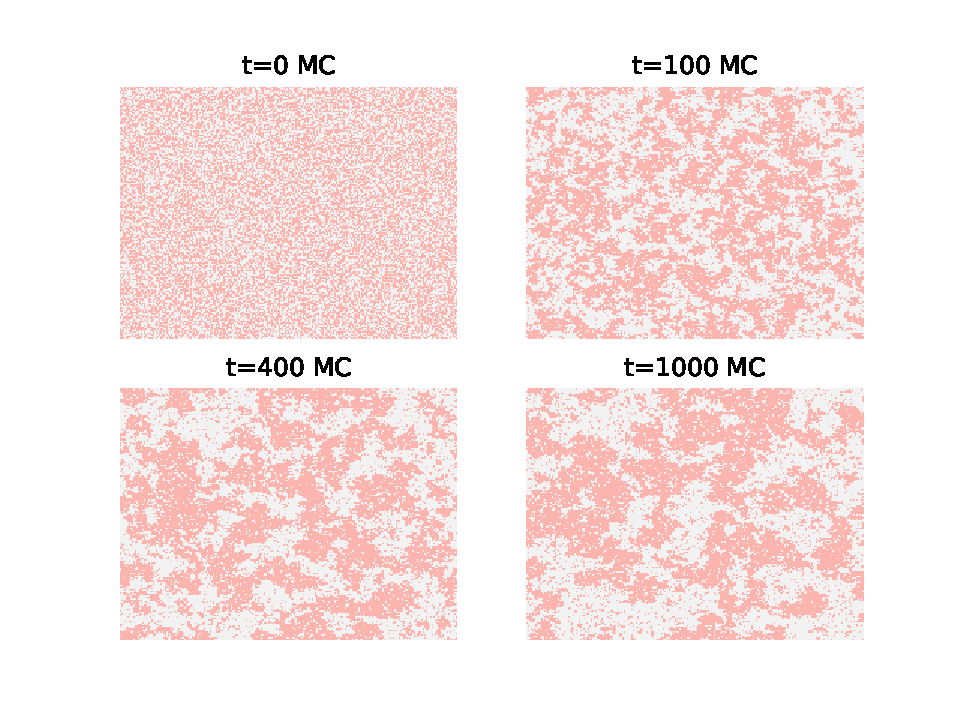
\includegraphics[width=\linewidth]{intro/clusterization.pdf}
    \caption{Numerical simulations of coarsening from a quench from a disordered state $T=\infty$ to an ordered state $T=T_{2D,C}$ \cite{onsager_crystal_1944} for different times, in Monte Carlo steps, for a $600 \times 600$ system with non-conserved Glauber dynamics.}
    \label{clusterization}
\end{figure}

While the phase diagram of a system can be determined via its Hamiltonian and equilibrium statistical mechanics, the dynamics of coarsening depends on the details of the systems dynamics that do not show up in single time thermodynamic observables. Therefore, one needs to construct dynamical models that capture the underlying evolution of the state of the system. In particular, there is a big difference between systems where the order parameter is conserved and those where it is not conserved.
%%%%%%%%%%%%%%%%%%%%%%
    \section{Models for equilibrium fields}
%%%%%%%%%%%%%%%%%%%%%%    

%%%%%%%%%%%%%%%%%%%%%%
    \subsection{Statics of systems with a finite number of degrees of freedom}
%%%%%%%%%%%%%%%%%%%%%%


Thermodynamic systems are naturally described in terms of fields, for example densities. 

Measuring observables in experimental setups means to measure the derivative of the partition function $Z$ with respect to its conjugate variable. This measure is done with a certain degree of spatial and temporal resolution, which means in a statistical language that they measure the average of the observable over some space and time. If $\Phi(\bx,t)$ is the physical field of our system, our device having a temporal resolution of $dt$ and a spatial resolutoin over a volume $V$ will measure
\begin{align}
\phi(\bx,t) = \frac{1}{V dt} \int_{t-dt}^{t} dt' \int_V \bx' \Phi(\bx',t')
\label{renormalisation}
\end{align}


This means that one is naturally lead to consider statistical field theories where the system is described in terms of a local field $\phi(\bx)$. Statistical field theories can be applied to both statics, to understand phase diagrams, and dynamics to understand phase ordering. However to start with we will examine the case of systems with a finite number of degrees of freedom. 

Consider a system in the canonical ensemble with a Hamiltonian $H(\bq)$ where $q_i$ for 
$1\leq i\leq N$ represent a finite number of continuous spatial degrees of freedom and where in a classical system we have already integrated over the corresponding momenta. The partition function for the system is given by
\begin{equation}
Z = \int d\bq \exp\left(-\beta H(\bq)\right)
\end{equation}
In general the integral which gives the partition function cannot be computed analytically. In equilibrium, the probability density function $P_{eq}(\bq)$ of the degrees of freedom is given by 
\begin{equation}
P_{eq}(\bq) = \frac{\exp\left(-\beta H(\bq)\right)}{Z}
\label{eqdis}
\end{equation}

The simplest approximation to compute $Z$ is the mean field approximation where the integral 
is approximated by the integrand at its largest value - in mathematics this is the Laplace method for approximating an integral and in this context it is just an expansion about the minimum energy configuration of the system. The mean field approximation is thus
\begin{equation}
Z_{MF}= \exp\left(-\beta H(\bq^*)\right)
\end{equation}
where $\bq^*$ is the value of $\bq$ which minimises $H$ (note that the approximation becomes exact in the zero temperature limit - $\beta \to \infty$ - as the system will minimise its energy). The values $q_i^*$ are determined from
\begin{equation}
\frac{\partial H}{\partial q_i}|_{\bq={\bf q^*}}=0
\end{equation}
Within this approximation any thermodynamic observable is given by
\begin{equation}
< f(\bq) > = f(\bq^*)
\end{equation}

We now consider how one can model dynamics of such systems. We will look for a Langevin equation which is chosen to give the correct equilibrium Gibbs-Boltzmann distribution. We write
\begin{equation}
\frac{d q_i}{dt} = -L_{ij}\frac{\partial H(\bq)}{ \partial q_j} + \eta_i(t)
\end{equation}
where $L_{ij}$ is a matrix which discuss later and $\eta_i(t)$ is zero mean Gaussian white noise with correlation function 
\begin{equation}
< \eta_i(t)\eta_j(t')> = \Gamma_{ij} \delta(t-t')
\label{cfn}
\end{equation}
The Gaussian white noise represents the effects of thermal fluctuations on the system we assume that the correlation time of these fluctuations is extremely short with respect to the dynamics of the degrees of freedom $q_i$ (in fact in critical systems the dynamics become very slow, critical slowing down, and this approximation becomes better and better as one approaches the critical point). There is no momentum term in this Langevin equation and for this reason it is often called the overdamped Langevin equation. Overdamped Langevin equations can also be derived staring from Newton's laws in the presence of friction, due to a solvent, and again white noise (again due to molecular collisions with the solvent) and by taking the limit where the frictional forces are greater than the acceleration term in Newton's equations (equivalent to setting the particle masses to zero).


As Eq. (\ref{cfn}) is for a correlation function the matrix $\Gamma_{ij}$ must be symmetric and cannot have any negative eigenvalues.

In the absence of noise or thermal fluctuations, so at zero temperature, the system will simply minimise its energy. Therefore if 
\begin{equation}
\frac{\partial H(\bq)}{ \partial q_j} =0
\end{equation}
with no noise we have $\frac{d q_i}{dt}=0$, that is to say it is the term $\frac{\partial H(\bq)}{ \partial q_j}$ that drives the dynamics if there is no noise. As long as the matrix $L_{ij}^{-1}$ exists the zero temperature dynamics will take the system to the local minimum of $H$ and to the absolute minimum if there are no metastable configurations. 


Under these assumptions, the Fokker-Planck equation for the probability density function of the degrees of freedom is 
\begin{equation}
\frac{\partial p(\bq,t)}{\partial t} = \frac{\partial}{\partial q_i} \left[\frac{1}{2}\Gamma_{ij} \frac{\partial p(\bq,t)}{\partial q_i} + p(\bq,t) L_{ij}\frac{\partial H(\bq)}{ \partial q_j}\right]
\end{equation}
This can be written as 
\begin{equation}
\frac{\partial p(\bq,t)}{\partial t} +\frac{\partial}{\partial q_i}J_i(\bq,t)=0
\end{equation}
where the ${\bf J}(\bq,t)$ is the probability current. We now insist that the system is in equilibrium with zero current when $p(\bq,t)= P_{eq}(\bq)$ as given by Eq. \eqref{eqdis}, this gives
\begin{equation}
\left[-\frac{\beta}{2}\Gamma_{ij} + L_{ij}\right]\frac{\partial H(\bq)}{ \partial q_j}
\end{equation}
and this holds for any choice of $H$ is we chose
\begin{equation}
\Gamma_{ij}= 2T L_{ij}
\end{equation}
where we have taken units where Boltzmann's constant $k_B=1$. 

%%%%%%%%%%%%%%%%%%%%%%
\subsection{Statistical field theory}
%%%%%%%%%%%%%%%%%%%%%%

We now consider a system with Hamiltonian $H[\phi]$ which depends on a continuous field $\phi(\bx)$. The partition function is given by a functional integral
\begin{equation}
Z = \int d[\phi] \exp(-\beta H[\phi]),
\end{equation}
the functional integral over all possible fields $\phi$ can be taken as a limit where $\phi$ is defined at a finite number of points on a lattice and then the lattice spacing is taken to zero. 
In many cases, the system has been coarse grained and $\phi$ represents a spatially varying order parameter, for instance the local density averaged over some small volume. In this case the Hamiltonian $H$ is strictly speaking a free energy and contains terms that depend on the temperature.

The mean field approximation to partition function is then given by
\begin{equation}
Z _{MF}= \exp(-\beta H[\phi_{MF}])
\end{equation} 
where $\phi_{MF}$ is the mean field solution which minimises $H$. The definition of a functional derivative of a functional is
\begin{equation}
F[\phi+\delta\phi]-F[\phi]= \int d\bx \frac{\delta F}{\delta\phi(\bx)} \delta\phi(\bx)
\end{equation}
Therefore if a field $\phi$ maximises $H$ we must have 
\begin{equation}
\frac{\delta H}{\delta\phi(\bx)}=0
\end{equation}

We now consider the standard Landau-Ginzburg Hamiltonian \cite{l_landau_physique_1990} describing Ising like systems where
\begin{equation}
H[\phi] = \int d\bx \ \frac{\kappa}{2}[\nabla \phi]^2 + V(\phi)
\label{landau-ginzburg-hamiltonian}
\end{equation}

The first term represents an energetic cost of varying the field $\phi$. The second potential term has two minima at $\phi=\pm \phi_c$, and, in the low temperature or phase separated phase, without loss of generality we can chose $V(\phi_c)=V(-\phi_c)$, while it has a single minimum at $\phi=0$ in the high temperature phase.

The standard potential for phase separations, called the $\phi^4$ model, is given by the double-well
\begin{align}
V(\phi) = \frac{1}{2} m^2 \phi^2 + \frac{\lambda}{4!} \phi^4
\label{phi4}
\end{align} 
where $m^2 = T-T_C$. For $m^2 \less 0$, the minima are at $\phi_C = \pm \sqrt{- \frac{6 m^2}{\lambda} } \pm$, while at $m^2 \ge 0$, the single minimum is at $\phi_C = 0$. We can also couple our system with the magnetic field of Hamiltonian
\begin{align}
H_1 &= - \int d^dx h(\bx)\phi(\bx)
\label{champ-externe}
\end{align}
As we in Fig \ref{double-puits-temperature}, the addition of an uniform external field does favour one phase over the other one.


\begin{figure}
\centering
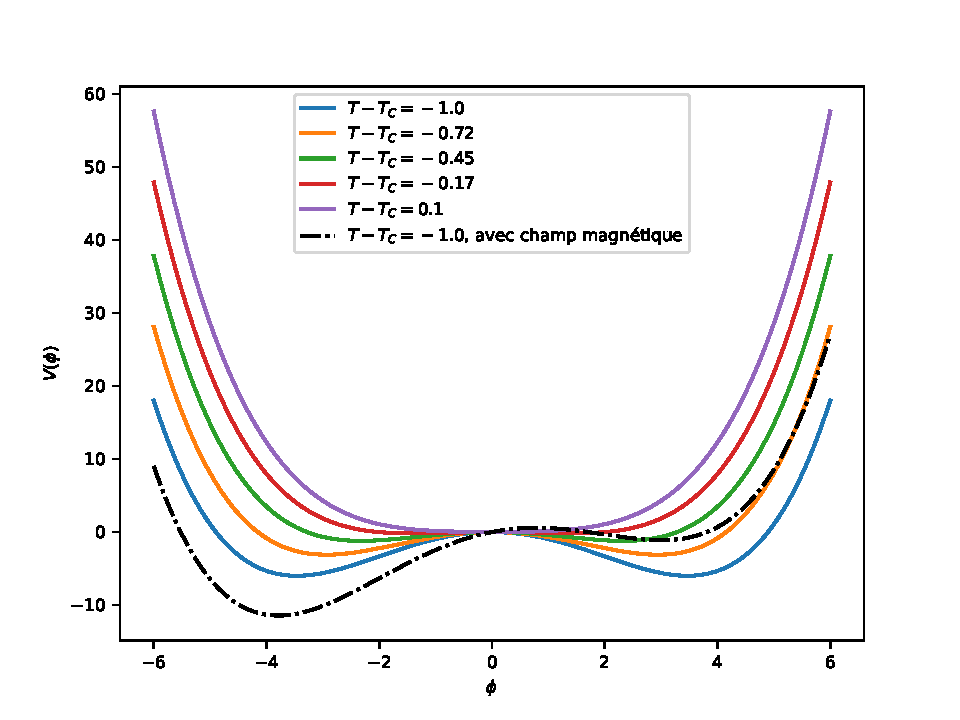
\includegraphics[width=0.6\linewidth]{intro/double-puit-en-fonction-temp.pdf}
\caption{Double-well potential \eqref{phi4} for $\lambda=1$ in function of the temperature difference with respect to the critical temperature with $m^2 = T-T_C$. In the ordered phase, the minima are at $\phi_C =\pm \sqrt{- \frac{6 m^2}{\lambda} } $, while for the ordered phase it is at $\phi_C = 0$. In black, the addition of a uniform magnetic field $h(\bx) = 1$ makes the positive phase metastable.}
\label{double-puits-temperature}
\end{figure}

It is easy to see that 
\begin{equation}
\frac{\delta H}{\delta \phi(\bx)} = -\kappa \nabla^2 \phi(\bx) + V'(\phi)
\label{cm}
\end{equation}
If we compare with systems with a discrete number of variables we
should have a Langevin equation of the form
\begin{equation}
\frac{\partial \phi(\bx)}{\partial t}= -L \frac{\delta H}{\delta \phi(\bx)} + \eta(\bx,t)
\end{equation}
The white noise correlator should have the form
\begin{equation}
< \eta(\bx,t)\eta(\bx',t)> =\delta(t-t')\Gamma(\bx,{\bf x'}),
\end{equation}
where here $\Gamma(\bx,{\bf x'})$ is an operator (before it was a matrix) defined by its action on functions $f$ as
\begin{equation}
\Gamma f(\bx) = \int d\bx' \Gamma(\bx,\bx')f(\bx')
\end{equation}
and $L$ is also an operator with 
\begin{equation}
L f(\bx) = \int d\bx' L(\bx,\bx')f(\bx')
\end{equation}
Following the same arguments for systems with a finite number of degrees of freedom we thus have the relation (which is sometimes called the fluctuation dissipation theorem as it essentially is equivalent)
\begin{equation} 
\Gamma(\bx,\bx') =2T L(\bx,\bx')
\label{gnoise}
\end{equation}

The simplest form of dynamics is given by $L(\bx,\bx')=\alpha\delta(\bx-\bx')$ which gives the \textbf{model A dynamics}
\begin{equation}
\frac{\partial \phi(\bx)}{\partial t}= -\alpha \frac{\delta H}{\delta \phi(\bx)} + \eta(\bx,t) 
\label{MA}
\end{equation}
with the noise correlator
\begin{equation}
< \eta(\bx,t)\eta(\bx',t)> =2T \alpha \delta(t-t')\delta(\bx-{\bf x'})
\end{equation}
The average value of $\phi$ 
\begin{equation}
\overline \phi(t) = \frac{1}{V}\int d\bx\ \phi(\bx,t)
\end{equation}
is clearly not generally conserved by this dynamics. Model A corresponds to a system in the grand-canonical ensemble, where $\alpha$ is the kinetic coefficient related to the relaxation time of the system \cite{hohenberg_theory_1977}.

\textbf{Model B dynamics} amounts to choosing
\begin{equation}
L(\bx-\bx')= -D\nabla^2 \delta(\bx-{\bf x'})
\end{equation}
The fact that $L$ is a positive semi-definite operator can be seen by taking its Fourier transform. The evolution equation here is
\begin{equation}
\frac{\partial \phi(\bx)}{\partial t}= D\nabla^2 \frac{\delta H}{\delta \phi(\bx)} + \eta(\bx,t)
\label{MB}
\end{equation}
where
\begin{equation}
< \eta(\bx,t)\eta(\bx',t)> =-2TD \delta(t-t')\nabla^2\delta(\bx-{\bf x'})
\end{equation}
We notice that if we introduce the vectorial white noise with components $\eta_i(\bx,t)$ such that
\begin{equation}
< \eta_i(\bx,t) \eta_i(\bx',t')> =\delta_{ij} \delta(\bx-{\bf x'})\delta(t-t)
\end{equation}
where $\delta_{ij}=1$ for $i=j$ and is zero otherwise, we can write
\begin{equation}
\eta(\bx,t)= \nabla\cdot {\boldsymbol \eta}(\bx,t)
\end{equation}
as one can verify the two noises have the same correlation function. In this way Eq. \eqref{MB} becomes 
\begin{equation}
\frac{\partial \phi(\bx)}{\partial t}= \nabla\cdot[ D\nabla \frac{\delta H}{\delta \phi(\bx)} + {\boldsymbol\eta}(\bx,t)]
\end{equation}
From this it is easy to see that the order parameter is conserved - thus model B describes conserved phase ordering dynamics. This model corresponds to the canonical ensemble, and is useful to describe diffusion or accretion systems.

Without the noise fluctuations, equations \eqref{MA} and \eqref{MB} are called the Time Dependant Ginzburg-Landau equation \cite{tuszynski_exact_1984} and the Cahn-Hilliard equation\cite{cahn_free_1958} equations, which give the mean field's dynamics.


%%%%%%%%%%%%%%%%%%%%%
\subsection{Surface tension}
%%%%%%%%%%%%%%%%%%%%%

In order to minimize the free energy in a non-conserved system, we can simply choose $\phi(\bx) =\phi_c$ or $\phi(\bx) =-\phi_c$ everywhere, which corresponds to a free energy $F=H[\phi_c]=0$. However in a system with a conserved order parameter
\begin{equation}
\int d\bx \ \phi(\bx)=0
\end{equation}
the solutions $\phi=\pm \phi_c$ cannot hold. In this case the system will separate into two homogeneous phases where $\phi(\bx)= \pm \phi_c$. We therefore choose an interface at $z=0$ and take $\phi(\bx) = \phi_K(z)$ ($K$ standing for kink as it is known as the kink solution in the literature) where $\lim_{z\to\-\infty}=-\phi_c$ and $\lim_{z\to\infty}=-\phi_c$. 
We therefore find from Eq. \eqref{cm} that
\begin{equation}
-\kappa \frac{d^2 }{dz^2}\phi_K(z) + V'(\phi_K) = 0 
\label{kk0}
\end{equation}
We can write
\begin{equation}
H[\phi_K]= A\int dz \ \frac{\kappa}{2}\left(\frac{d\phi_K(z)}{dz}\right)^2 + V(\phi_K(z))
\label{kk1}
\end{equation}
where $A$ is the surface area of the system in the plane perpendicular to the direction $z$. 
However, if we multiply Eq. \eqref{kk0} by $d\phi/dz$ and integrate we find
\begin{equation}
-\frac{\kappa}{2} (\frac{d\phi_K}{dz})^2 + V(\phi_K) = C
\end{equation}
where $C$ is a constant. However as $\phi_K(z)\to \pm \phi_c$ as $z\to \pm \infty$ and $V(\pm\phi_c) =0$ we find that $C=0$. Using this, we obtain 
\begin{equation}
H[\phi_K]= A\int dz\ {\kappa}\left(\frac{d\phi_K(z)}{dz}\right)^2 
\end{equation}
If the interface has a free energy per unit area of $\sigma$ then we have the Cahn-Hillard estimate of the surface tension \cite{cahn_free_1958}
\begin{equation}
\sigma= \int dz\ {\kappa}\left(\frac{d\phi_K(z)}{dz}\right)^2 
\label{CHST}
\end{equation}

In the case of the $\phi^4$ model defined at Eq \eqref{phi4}, the equation \eqref{kk0} becomes
\begin{align}
\kappa \phi_K''(z) = m^2 \phi_K(z) \left( 1 + \phi_C \phi_K(z) ^2 \right)
\label{eq-interface-glauber}
\end{align}
This potential is only defined by the ratio between $m^2$ and $\lambda$, so without loss of generality we set $\phi_C = 1$. The solution becomes
\begin{align}
\phi_K(z) = \tanh \left( \frac{z}{\xi} \right)
\label{profil-interface-glauber} 
\end{align}
where $\xi = \sqrt{\frac{-2 \kappa}{m^2}}$. This correlation length diverges when $T\to T_C$.
From Fig \ref{tension-xi} we see that the bigger the correlation length of the system, the smaller the surface tension is. The experimental study of quasi-critical systems, which have fluctuations at a macroscopic length scale, is a good way to probe the properties of ultra-low surface tension systems \cite{hennequin_drop_2006}. Such systems are very susceptible to hydrodynamic instabilities caused by thermal noise, as in microfluidics for example \cite{atencia_controlled_2005}. 
\begin{figure}
\centering
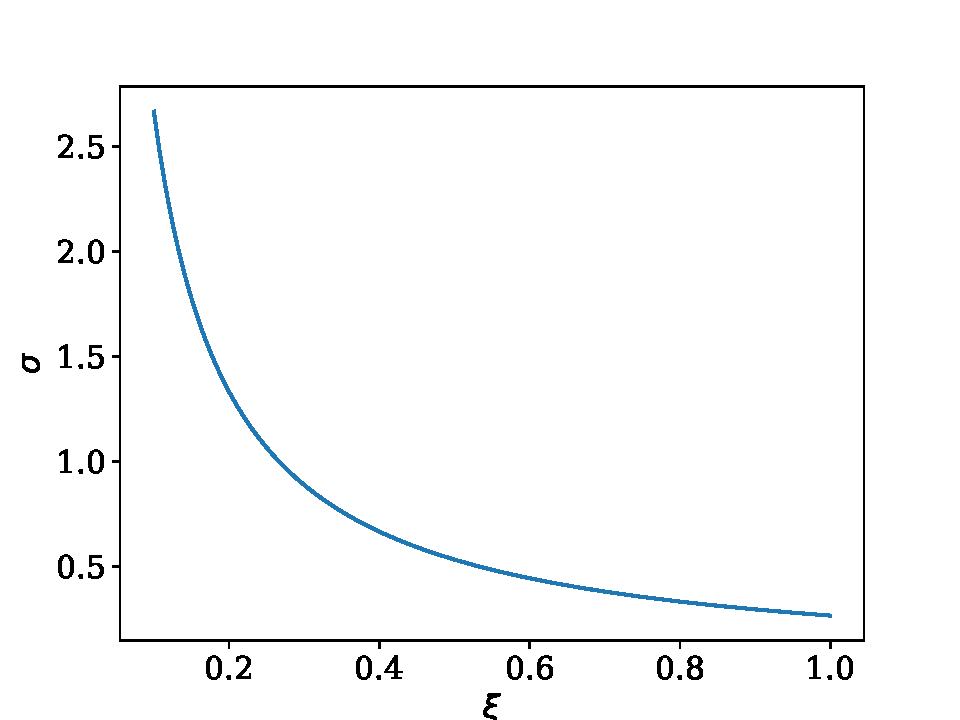
\includegraphics[width=0.7\linewidth]{int-dyn/tension-superficielle.pdf}
\caption{Superificial tension \eqref{CHST} with respect to $\xi$ for the $\phi^4$ solution \eqref{profil-interface-glauber}.}
\label{tension-xi}
\end{figure}


%%%%%%%%%%%%%%%%%%%%%%
\section{Models for equilibrium interfaces}
\label{sec-continuous}
%%%%%%%%%%%%%%%%%%%%%%

%%%%%%%%%%%%%%%%%%%%%%
\subsection{Basic continuous model}
%%%%%%%%%%%%%%%%%%%%%%

Here we discuss effective models of interfaces. The simplest model is to assume that the 
interface is parameterised by a height profile $h(\br)$, where $\bx = (\br,z)$ however one also has to assume that 
$h(\br)$ is a single-valued function of $\br$. Given this one can write
\begin{equation}
H[h] = \sigma A[h]
\end{equation}
where $A_h$ is the area of the interface. However, the interface area is given by
\begin{equation}
A[h] = \int_A d\br\sqrt{1+[\nabla h]^2}
\end{equation}
where the integral is over the plane perpendicular to the $z$ axis which is taken to be of area $A$. When the fluctuations of the interface are small, we can expand the above to quadratic order in $h$ to obtain
\begin{equation}
H[h]= A\sigma +\frac{\sigma}{2} \int_A d\br \ [\nabla h]^2
\end{equation}
The first term is independent of the height, so we can write the effective Hamiltonian for the surface as
\begin{equation}
H_{eff} [h]= \frac{\sigma}{2} \int_A d\br\ [\nabla h]^2
\label{heff}
\end{equation}

The basic model describing the height of an interface at $z=h(\br)$ above a plane with coordinates $\br$ has the Hamiltonian 
\begin{equation}
H[h] = \int d\bx\frac{\sigma}{2} [\nabla h(\bx)]^2 + V(h(\bx))
\end{equation}
The first term corresponds to the surface energy for a surface of size $A_s$ 
\begin{equation}
H_s[h] = \sigma A_s =\sigma\int d\bx \sqrt{1+[\nabla h(\br)]^2}\approx \sigma A + \frac{\sigma}{2}\int d\br [\nabla h(\br)]^2 
\end{equation}
Here $A$ is the area of the projected plane below the surface which is taken to be constant and thus does not change the statistical mechanics of the system. In principle surfaces can also have bending energies, while surface energies correspond to stretching the surface to increase its size, bending energies correspond to curving the surface. The standard bending energy for small surface energies \cite{diehl_interface_1980} is given by
\begin{equation}
H_b[h] = \int d\br \frac{\kappa_b}{2}[\nabla^2 h(\br)]^2
\end{equation} 
where $\kappa_b$ is called the bending rigidity.

The term $V(h)$ is taken to represent the potential energy of the surface. For instance if the surface interacts via an infinite hard-core potential with a solid surface at $z=0$, this can be modelled by the potential $V(z) =0$ for $z \greater 0$ and $V(z)=\infty$ for $z\leq 0$. Another example is where the surface describes the surface of a liquid such as water, again with a solid surface at $z=0$, in the presence of gravity the potential energy of the water column above the area 
element $d\bx$ is given by
\begin{equation}
\delta V = \int_0^{h(\br)} dz\ \rho g z = \frac{1}{2}\rho g h^2(\br)
\end{equation}
where $\rho$ is the (mass) density of the liquid. This then gives
\begin{equation}
H[h] = \int d\br \frac{\sigma}{2}[\nabla h(\br)]^2 + \frac{1}{2}\rho g h^2(\br)
\end{equation}
We see that the correlation length of the interface is given by
\begin{equation}
\xi = \left(\frac{\sigma}{\rho g}\right)^{\frac{1}{2}}
\end{equation}
In the more general context, if $V(h)$ has a minimum at some point $h_m$ we can write $h= h_f(\bx)+ h_m$, where $h_f(\bx)$ represents the height fluctuations about the mechanically stable flat interface $h(\bx)=h_m$. Now expand assuming that $h_f(\bx)$ is
small we find the effective Hamiltonian for the fluctuations
\begin{equation}
H_{eff}[h_f] = \int d\br \frac{\sigma}{2}[\nabla h_f(\br)]^2 + \frac{1}{2}V''(h_m) h_f^2(\br)
\end{equation}
where we have dropped the constant term $AV(h_m)$. The above field theory is Gaussian and 
so, when the approximations made to derive it are valid, all of the statistical properties of the height fluctuations can be deduced. However for general potentials $V(h)$ the model cannot be solved exactly in two dimensions but can in principle be solved in one dimension as we will see below.

%%%%%%%%%%%%%%%%%%%%%%
\subsection{Effective dynamics of interface heights}
\label{sec-heightd}
%%%%%%%%%%%%%%%%%%%%%%
We will now try and derive an approximation for the dynamics of the height of the interface from the original phase ordering kinetics. Here we use the method of Bray and Cavagnha \cite{bray_interface_2001,bray_interface_2001-1}, which was used to study the dynamics of sheared interfaces, in the absence of shear to determine the dynamical properties of interfaces in phase separated systems for both model A and model B dynamics.

We imagine that the system is phase separated in the direction $z$, on average the interface is taken to be at $z=0$, and we write
\begin{equation}
\phi(z,\br,t) = f(z-h(\br,t))
\label{hans}
\end{equation}
where $f(z)=\phi_K(z)$ is the kink solution from mean field theory.

%%%%%%%%%%%%%%%%%%
\subsubsection{Model A dynamics}
%%%%%%%%%%%%%%%%%%

For model A dynamics, we substitute Eq. \eqref{hans} into Eq. \eqref{MA} and make use of the following results
\begin{align*}
\frac{\partial f(z-h(\br,t))}{\partial t} =& -f'(z-h(\br,t))\frac{\partial h(\br,t)}{\partial t}\\
\nabla f(z-h(\br,t) =& [{\bf e}_z-\nabla h(\br,t)]f'(z-h(\br,t)) \\
\nabla^2 f(z-h(\br,t))=& f''(z-h(\br,t))- \nabla^2 h(\br,t)f'(z-h(\br,t))+ [\nabla h(\br,t)]^2 f''(z-h(\br,t))
\end{align*}
and thus find
\begin{align*}
-f'(z-h(\br,t))\frac{\partial h(\br,t)}{\partial t}=& \alpha\kappa 
\left[ f''(z-h(\br,t))- \nabla^2 h(\br,t)f'(z-h(\br,t))+ [\nabla h(\br,t)]^2 f''(z-h(\br,t))\right] \\
& - \alpha V'(f'(z-h(\br,t))) + \eta(\br,z,t)
\end{align*}
We now multiply both sides of this equation by $f'(z-h(\br,t))$ and defining $\zeta=z-h(\br,t)$, we integrate $\zeta$ over $[-\infty,\infty]$ while using the following identities
\begin{align*}
\int_{-\infty}^\infty d\zeta f'(\zeta)f''(\zeta) =& [\frac{1}{2}f'^2(\zeta)]_{-\infty}^\infty =0 \\
\int_{-\infty}^\infty d\zeta f'(\zeta) V'(f) =& \int_{-\infty}^\infty d\zeta\frac{d V(f)}{d\zeta} =[V(f(\zeta))]_{-\infty}^\infty=0
\end{align*} 
Note that the first relation above holds as $f(\zeta)=\pm \phi_c$ as $\zeta\to\pm \infty$ and the second as
$V(\phi_c)=V(-\phi_c)=0$.
The terms that are left then give
\begin{equation}
-\int_{-\infty}^\infty f'^2(\zeta)d\zeta\ \frac{\partial h(\br,t)}{\partial t}
= -\alpha\int_{-\infty}^\infty f'^2(\zeta)d\zeta \ \kappa \nabla^2 h(\br,t) + \int_{-\infty}^\infty d\zeta \eta(\br,\zeta+ h(\br,t))f'(\zeta)
\end{equation}
Now using the Cahn-Hillard estimate of the surface tension, Eq. \eqref{CHST} thus becomes
\begin{equation}
\frac{\sigma}{\kappa} \frac{\partial h(\br,t)}{\partial t} = \alpha\sigma \nabla^2 h(\br,t) +\xi(\br,t)
\end{equation}
where the noise term is given by
\begin{equation}
\xi(\br,t)= \int_{-\infty}^\infty d\zeta \eta(\br,\zeta+ h(\br,t))f'(\zeta)
\end{equation}
The noise term has zero mean and correlation function
\begin{align}
< \xi(\br,t)\xi(\br',t')> =&2\alpha T\delta(t-t')\delta(\br-\br')\int_{-\infty}^\infty d\zeta d\zeta' \delta(\zeta-\zeta')f'(\zeta)f'(\zeta')\nn
=& 2\alpha T\delta(t-t')\delta(\br-\br')\int_{-\infty}^\infty d\zeta f'^2(\zeta)= \frac{2\alpha T\sigma}{\kappa}\delta(t-t')\delta(\br-\br')
\end{align}
This now gives
\begin{equation}
\frac{\partial h(\br,t)}{\partial t}= \kappa\alpha \nabla^2 h(\br,t) + \eta(\br,t)
\end{equation}
where 
\begin{equation}
< \eta(\br,t)\eta(\br',t')> = \frac{2\alpha T\kappa}{\sigma}\delta(t-t')\delta(\br-\br')
\end{equation}
Now defining $\alpha' = \frac{\kappa\alpha}{\sigma}$ we can write
\begin{equation}
\frac{\partial h(\br,t)}{\partial t}= \alpha' \sigma\nabla^2 h(\br,t) + \eta(\br,t)
\end{equation}
This has the form of model $A$ dynamics (as in Eq. \eqref{MA}) for the height profile with Hamiltonian
$H_{eff}$ as given in \eqref{heff}, that is to say we can write
\begin{equation}
\frac{\partial h(\br,t)}{\partial t}= -\alpha' \frac{\delta H_{eff}[h]}{\delta h(\br)} + \eta(\br,t)
\label{ew}
\end{equation}
with
\begin{equation}
< \eta(\br,t)\eta(\br',t')>= 2T\alpha'\delta(t-t')
\end{equation}
This dynamical calculation is thus consistent with the idea of describing the surface in terms of a height variable with an energy given by the surface tension. The equation \eqref{ew} is known as the Edwards-Wilkinson equation \cite{edwards_surface_1982,halpin-healy_kinetic_1995}. We can use this equation to determine how the domains of a coarsening system grow at low temperatures. To do this we ignore the noise term and assume that at $t=0$ the correlations of the height are short range. so
\begin{equation}
C(\br-\br',0)= < h(\br,0)h(\br',0)> =C_0 \delta(\br-\br')
\end{equation}
In Fourier space the noiseless Edwards-Wilkinson equation becomes
\begin{equation}
\frac{\partial\tilde h(\bk,t)}{\partial t} = -\alpha'\sigma \tilde h(\bk,t) 
\end{equation}
and so we find
\begin{equation}
\tilde h(\bk,t) = h(\bk,0)\exp(-\alpha'\sigma\bk^2 t)
\end{equation}
The two point correlation function becomes
\begin{equation}
< \tilde h(\bk,t)\tilde h(\bk',t')> = < h(\bk,0)h(\bk',0)> \exp(- \alpha'\sigma[k^2+k'^2] t)
\end{equation}
Now recall that if 
\begin{equation}
< h(\br,t) h(\br',t')> =C(\br-\br',t)
\end{equation}
then
\begin{equation}
< \tilde h(\bk,t)\tilde h(\bk',t')>= (2\pi)^d \delta(\bk+\bk') \tilde C(\bk,t)
\end{equation}
where 
\begin{equation}
\tilde C(\bk,t)= \int d\br \exp(-i\bk\cdot \br)C(\br,t)
\end{equation}
is the Fourier transform of the correlation function, which is a function of a single position due to invariance by translation in space, and $d$ is the dimension of space (so here $d=2$ for a surface in 3d space and $d=1$ for a surface in a 2d space). Putting all this together gives
\begin{equation}
\tilde C(\bk,t)= C_0 \exp(-2\alpha'\sigma k^2 t)
\end{equation}
Inverting the Fourier transform, we have
\begin{equation}
C(\br,t)= \frac{C_0}{(8\pi \alpha'\sigma t)^{\frac{d}{2}}} \exp(-\frac{\br^2}{16\pi \alpha'\sigma t})
\end{equation}
From this we see that if $C(\br,t)\sim g(\frac{\br}{\ell(t)})r(t)$ then the length scale $\ell(t)\sim t^{\frac{1}{2}}$, this agrees with what is found in the Ising model under Glauber dynamics, where the growth exponent is also given by $z=\frac{1}{2}$\cite{paul_domain_2005}.

%%%%%%%%%%%%%%%
\subsubsection{Model B dynamics}
%%%%%%%%%%%%%%

For model B dynamics, we take the same ansatz as in Eq. \eqref{hans} but we rewrite the model B dynamics as
\begin{equation}
-\nabla^{-2} \frac{\partial\phi(\bx,t)}{\partial t} = -D \frac{\delta H}{\delta \phi(\bx)}+ \theta(\bx,t)
\end{equation}
here $-\nabla^{-2}$ represents the Green's function $G$ which obeys 
\begin{equation}
\nabla^2 G(\bx-{\bf x'}) = -\delta(\bx-\bx')
\end{equation}
and 
\begin{equation}
\theta(\bx,t)=-\nabla^{-2}\eta(\bx,t)= \int d\bx'G(\bx-{\bf x'})\eta(\bx,t)
\end{equation}
The correlation function of $\theta(\bx,t)$ is given by
\begin{align}
< \theta(\bx,t)\theta({\bf y},t')> =&-2DT\delta(t-t') \int d\bx'G(\bx-{\bf x'})d{\bf y}'G({\bf y}-{\bf y'})\nabla^2\delta(\bx'-{\bf y}') \nn
=& -2DT\delta(t-t') \int d\bx'G(\bx-{\bf x'})d{\bf y}'\nabla^2G({\bf y}-{\bf y'})\delta(\bx'-{\bf y}') \nn
=& 2DT\delta(t-t') G(\bx-{\bf y})
\end{align}
where we have integrated by parts in the second line and used 
\begin{equation}
-\nabla^2G({\bf y}-{\bf y'})= \delta({\bf y}-{\bf y}')
\end{equation}
in the third.

Now multiplying by $f'(z-h(\br,t))$ and integrating $z$ over $[-\infty,\infty]$, we find
\begin{align}
-\int dz f'(z-h(\br,t))\int dz'd\br'\ G(z-z',\br-\br') f'(z'-h(\br',t))\frac{\partial h(\br',t)}{\partial t} = -D\sigma \nabla^2 h(\br,t) + \chi(\br,t),
\end{align}
with the noise
\begin{equation}
\chi(\br,t)= \int dz f'(z-h(\br,t)) \theta(\br,z,t).
\end{equation}
As we assume that the height fluctuations are small, we keep only the lowest order terms in $h$ in the deterministic terms and the noise, we will see later that this is compatible thermodynamically. We thus have
\begin{equation}
-\int dz \ f'(z)\int dz'd\br'\ G(z-z',\br-\br') f'(z')\frac{\partial h(\br',t)}{\partial t} = -D\sigma \nabla^2 h(\br,t) + \chi(\br,t)
\end{equation}
and now the noise is given by
\begin{equation}
\chi(\br,t)= \int dz\ f'(z) \theta(\br,z',t)
\end{equation}
This equation which is linear in $h$ can now be Fourier transformed in the plane $\br$. In terms of the Fourier transform of $h$ we find
\begin{equation}
-\int dz \ f'(z)\int dz'd\br'\ \tilde G(z-z',\bk) f'(z')\frac{\partial\tilde h(\bk,t)}{\partial t} = Dk^2\sigma \tilde h(\bk,t) + \tilde \chi(\bk,t)
\label{bstep}
\end{equation}
The Fourier transform of $G$ in the $\br$ plane obeys
\begin{equation}
\frac{d^2 \tilde G(z-z',\bk )}{dz^2}-k^2 \tilde G(z-z',\bk )=-\delta(z-z')
\end{equation}
and the solution to this equation (with the boundary condition that $\tilde G(z-z',\bk )\to 0$ as $|z-z'|\to\infty$) is
\begin{equation}
\tilde G(z-z',\bk) = \frac{\exp(-k|z-z'|)}{2k}
\end{equation}
where we note $k=|\bk|$. Next we make the sharp interface approximation where we write
\begin{equation}
f(z) = 2\phi_c \delta(z)
\label{sharp}
\end{equation}
that is to say we have replaced the smooth kink solution with a step like solution
$f(z) = \phi_c\ {\rm sgn}(z)$. This then gives
\begin{equation}
-4\phi_c^2 \tilde G(0,k) \frac{\partial h(\bk,t)}{\partial t} = Dk^2\sigma \tilde h(\bk,t) + \tilde \chi(\bk,t)
\end{equation}
which we rewrite as
\begin{equation}
\frac{\partial \tilde h(\bk,t)}{\partial t} = -\frac{Dk^3\sigma}{2\phi_c^2} \tilde h(\bk,t) + \tilde \xi(\bk,t)
\end{equation}
with 
\begin{equation}
\tilde \xi(\bk,t)= - \frac{k}{2\phi_c^2}\tilde \chi(\bk,t)
\end{equation}
where 
\begin{equation}
\tilde \chi(\bk,t)= \int dz\ f'(z) \tilde\theta(\bk,z,t)
\end{equation}
The correlation function of $\tilde \theta(\bk,t)$ is 
\begin{equation}
< \theta(\bk,t)\theta(\bk',t')> = 2DT(2\pi)^d \delta(t-t') \delta(\bk+{\bf k'}) \tilde G(z-z',k)
\end{equation}
From this we find 
\begin{equation}
< \chi(\bk,t)\chi(\bk',t')> = 2DT(2\pi)^d \delta(t-t') \delta(\bk+{\bf k'}) \int dz dz' f(z) f(z') \tilde G(z-z',k)
\label{bstep2}
\end{equation}
Now, using the sharp interface approximation Eq. \eqref{sharp}, we obtain
\begin{equation}
< \chi(\bk,t)\chi(\bk',t')> = 2DT(2\pi)^d \delta(t-t') \delta(\bk+{\bf k'}) \frac{2\phi_c^2}{k}
\end{equation}
and consequently
\begin{equation}
< \xi(\bk,t)\xi(\bk',t')> = 2DT(2\pi)^d \delta(t-t') \delta(\bk+{\bf k'}) \frac{k}{ 2\phi_c^2}
\end{equation}
Finally in we find the interface dynamics for model B in Fourier space is
\begin{equation}
\frac{\partial h(\bk,t)}{\partial t} = -\frac{Dk^3\sigma}{2\phi_c^2} \tilde h(\bk,t) + \tilde \xi(\bk,t)
\label{modBFT}
\end{equation}
In real space this has the form
\begin{equation}
\frac{\partial h(\br)}{\partial t}= -L \frac{\delta H_{eff}}{\delta h (\br)} + \xi(\br,t)
\end{equation}
where the operator $L$ is defined via its Fourier transform
\begin{equation}
\tilde L(\bk) = \frac{Dk}{2\phi_c^2}
\end{equation}
Now if we look at Eq. \eqref{modBFT} we see that solving the equation without noise will give a function of $k^3t$, which in real space corresponds to $x^3/t$. From this we see that the coarsening length scale grows as $\ell(t) \sim t^{\frac{1}{3}}$ and consequently the coarsening exponent is $z=\frac{1}{3}$. Coarsening for conserved model B or diffusive dynamics is slower than that of model A \cite{huse_corrections_1986}. One of the reasons for this slowing down with respect to nonconserved dynamics is that material must be physically transported by diffusion (by exchanging spins in the language of lattice spin models), where as for model A dynamics the composition can change at any given point by {\em spin flipping}. As a cautionary note, if we had taken the Hamiltonian in Eq. \eqref{heff} and applied model B conserved dynamics, as in Eq. \eqref{MB}, for the height field we would not have obtained this equation. 

We can actually do better than the above sharp interface approximation as Eq. \eqref{bstep} can be written as
\begin{equation}
Q(k)\frac{\partial\tilde h(\bk,t)}{\partial t} = -Dk^2\sigma \tilde h(\bk,t) - \tilde \chi(\bk,t)
\label{bstep2}
\end{equation}
where 
\begin{equation}
Q(k)= \int dzdz' \ f'(z)\ \tilde G(z-z',\bk) f'(z')
\end{equation}
Notice that from Eq. \eqref{bstep2} that
\begin{equation}
< \chi(\bk,t)\chi(\bk',t')> = 2DT(2\pi)^d \delta(t-t') \delta(\bk+{\bf k'}) Q(k)\end{equation}
and so 
\begin{equation}
\frac{\partial\tilde h(\bk,t)}{\partial t}= -\tilde L(k) \tilde \mu(\bk) + \eta(\bk)
\end{equation}
where $\mu(\bx)=\delta H_{eff}/\delta h(\bx) $, $\tilde L(k) = D/Q(k)$ and 
\begin{equation}
< \eta(\bk,t)\eta(\bk',t')> = 2T(2\pi)^d \delta(t-t') \delta(\bk+{\bf k'}) \tilde L(k)
\end{equation}

%%%%%%%%%%%%%%%%%%%
    \section{Lattice models}
%%%%%%%%%%%%%%%%%%%

%%%%%%%%%%%%%%%%%%%%%%%%%%%%%%%%%%%%%%%%%%%%%
    \subsection{The Ising model}
%%%%%%%%%%%%%%%%%%%%%%%%%%%%%%%%%%%%%%%%%%%%%  


We take a system of size $L'\times L' \times L$, composed of $N$ sites $i$. At each site corresponds a value $\sigma_i =\pm1$. The Hamiltonian of the Ising model is 
\begin{equation}
	H =  - \sum_{<ij>} J \sigma_i \sigma_j + \frac{V(\sigma_i)+V(\sigma_j)}{2}
	\label{hamil-ising}
\end{equation}
where $\sum_{< ij >}$ is a sum over all pairs of nearest neighbours, and the external field $V(\sigma_i)$ has been symmetrized. The Ising model\cite{niss_history_2005,niss_history_2009} is therefore a lattice model with short interactions between particles. Since all particles $\sigma_i$ in the system are equal to $\pm!$, this system is called a lattice based spin model. When $\sigma_i$ is continuous, it is called the XY model \cite{gupta_phase_1988}.
$J$ is called the coupling parameter of the system, and can be non-uniform, with the nearest neighbours interaction being $J = J_{ij}$. If $ J_{ij} =0$, the system favorises homogeneous phases and is called ferromagnetic. Otherwise, the system favorises configurations where each spin has an opposite sign with respect to all of their neighbours, which modelises antiferromagnetic materials. We will pose $J=1$.

\begin{figure}[t]
	\begin{minipage}[t]{0.5\linewidth}
		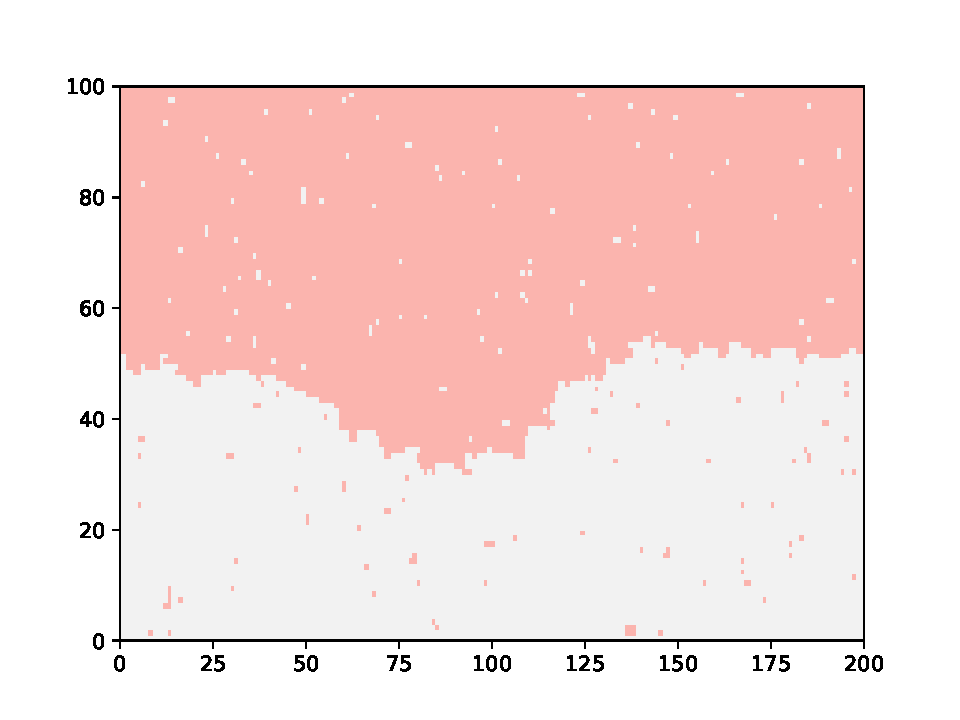
\includegraphics[width=\linewidth]{int-dyn/inte07.pdf}
	\end{minipage}%
	\begin{minipage}[t]{0.5\linewidth}
		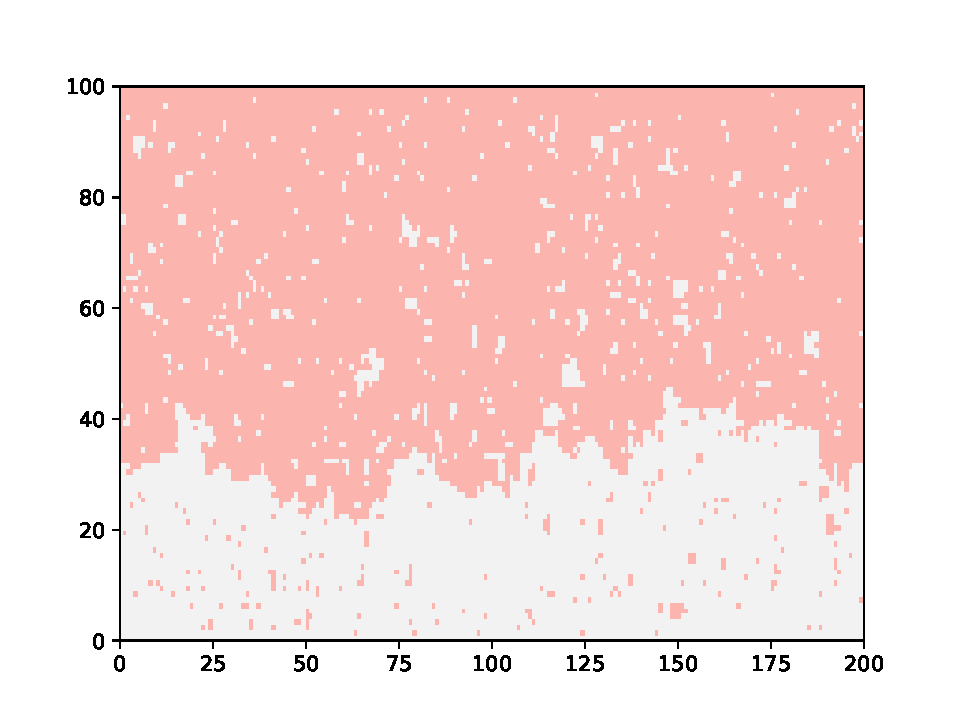
\includegraphics[width=\linewidth]{int-dyn/inte09.pdf}
	\end{minipage}
	\caption{Snapshot of Monte Carlo simulations of the Ising model for two different temperatures in two dimensions($T=0.7 T_C$ (left) and $T=0.95 T_C$ (right)) with periodic boundary conditions in $x$ and fixed ones in$y$.}
	\label{amas-fixe}
\end{figure}  


The mean-field theory with a $\phi^4$ potential has been developed from this model \cite{bellac_equilibrium_2004}. Exact relationship between both of them has been found in 4 dimensions and above \cite{aizenman_proof_1981}. A fast way to convince ourselves is to take the finite difference derivative at first order of Eq \eqref{landau-ginzburg-hamiltonian}. If we suppose the sole role of the potential is to set the field to $\pm \phi_C$ on each site, then we have
\begin{align}
    [{\boldsymbol \nabla} \phi(i)]^2 &= \left( \frac{\partial \phi(i)}{\partial x} \right)^2  + \left( \frac{\partial \phi(i)}{\partial y} \right)^2 + \left( \frac{\partial \phi({\bf i})}{\partial z} \right)^2\nn
    &= (\phi(x,y,z)-\phi(x+1,y,z))^2 + (\phi(x,y,z)-\phi(x,y+1,z))^2 + (\phi(x,y,z)-\phi(x,y,z+1))^2 \nn
    &= 2 (1-\phi(x,y,z)\phi(x+1,y,z) + 2 (1-\phi(x,y,z)\phi(x,y+1,z) +2 (1-\phi(x,y,z)\phi(x,y,z+1) 
    \label{discretisation-landau}
\end{align}
where we've set the distance between two sites to $1$.
From this we easily see some bulk energy to which we add the sites' nearest neighbours interactions in an Ising-like fashion.
%%%%%%%%%%%%%

This model precisely describes  phase transitions in uniaxial magnetic systems\cite{de_jongh_experiments_1974,wp_wold_ising_2000,ikeda_neutron_1973}. It is also the simplest model of its eponymous universality class, which also contains liquid/gas transitions and binary fluids.
In these mappings, $n_i=\frac{1}{2}(1-\sigma_i)=0,1$ represents occupation of a cell of a lattice fluid or $\sigma_i$ gives the label of a binary species $A$ or $B$.
This model does not have a phase transition in 1D, but a phase transition in 2D was foumd in 1944\cite{onsager_crystal_1944} at the critical temperature 
\begin{align}
     T_{2D,C} = \frac{2J}{k_B \ln(1 + \sqrt{2})} \simeq 2.27 \frac{J}{k_B}
\end{align}

The renormalization group approaches have a deep connexion with the Ising model \cite{frohlich_triviality_1981,goldenfeld_lectures_2018}. Even though results have been found for $d=4$ (which is the upper critical dimension), no analytical solution has been found in 3 dimensions. Numerous numerical simulations  \cite{talapov_magnetization_1996,preis_gpu_2009} have shown that the 3-dimensional phase transition occurs at 
\begin{align}
    T_{3D,C} \simeq 4.51 \frac{J}{k_B}
\end{align}


By doing the transformation\cite{goldenfeld_lectures_2018} 
\begin{align}
    n_i =  \frac{\sigma_i +1}{2}
\end{align}
so that $n_i(\sigma_i = 1) = 1$ and $n_i(\sigma_i = -1) = 0$, we obtain
\begin{equation}
	H =  - \sum_{< i j >}  J_{ij} \left( 4 n_i n_j -2 ( n_i+n_j) + 1 \right)+ \sum_{< i j >}  J_{ij} \frac{V(\sigma_i)+V(\sigma_j)}{2}  
\end{equation}
where the constant term $\sum_{< i j >}  J_{ij}$ does not change the partition function behaviour. We have then
\begin{align}
	H_{LG} &=  - 4 \sum_{< i j >}  J_{ij}  n_i n_j  + 2 \sum_{< i j >}  J_{ij}  (n_i+n_j) + \sum_{< i j >}  J_{ij} \frac{V(\sigma_i)+V(\sigma_j)}{2}  \nn
       &=  - 4 J \sum_{< i j >}  J n_i n_j  + \mu \sum_i  n_i + \sum_{< i j >}  J \frac{V(\sigma_i)+V(\sigma_j)}{2}  
\end{align}
where we have set $J_{ij} = J$ constant and defined the intrinsic chemical potential for a liquid-gas system as $\mu_c=4J c$, with  $c$ the number of nearest neighbours. A positive magnetic phase is thus analogous to a high density state such a liquid, while the negative magnetic phase is equal to a low density state such as a gas. An onsite potential $V(\sigma_i)$ further modifies the chemical potential, $\mu=\mu_c+\delta\mu[V(\sigma_i)]$.
The chemical potential $\mu$ is the conjugate variable to the total number of particles $\sum_i n_i$, while the magnetic field $B$ is the conjugate variable to the total magnetisation $\sum_i \sigma_i$. The two are connected through the mapping such that $B\sim \mu-\mu_c$, so that liquid-gas and Ising model systems share common thermodynamic features such as the universality class for critical fluctuations. For the fluid the grand canonical ensemble corresponds to the Gibbs ensemble with fixed $T$ and $\mu$ and canonical ensemble with fixed $T$ and $N$ . In the magnetic system these ensembles correspond to fixed $T, B$ and $T,M$ respectively. The model also describes adsorption of a gas in a lattice or binary fluids between particles of different species $A$ and $B$.



By imposing $+-$ boundary conditions in the $z$ direction, we force the existence of an interface Those BC can be fixed, imposing  $\sigma(z=0) = -1$ and $\sigma(z=L)=+1$, or free but with a local external field $V(z) = h (\delta_{0,z}-\delta_{z,L})$.
An interface is characterized by its mean and its width. The easiest way to do so is to fit the magnetization profile
\begin{align}
    m(z) = \frac{1}{L'^2} < \sum_{xy} \sigma(x,y,z) >
\end{align}
to mean field results from Eq \eqref{profil-interface-glauber} . The mean position of the interface is
\begin{align}
    m = <h> = \frac{1}{L'^2} < \sum_i \sigma_i >
\end{align}
The width of the interface is then defined  as 
\begin{align}
    w^2 = <h^2>-<h>^2
\end{align}
This can be rewrtiten \cite{stecki_magnetization_1994} as
\begin{align}
    w^2 = 2 \frac{ \int_0^L dz z \frac{d m(z)}{dz}}{\int_0^L dz \frac{d m(z)}{dz}}
\end{align}
We now defined the surface tension of the interface as the free energy difference between  the bulk and interface \cite{richards_numerical_1993}. Is $Z^{++}$ si the partition function of a system with $(++)$ BC, and $Z^{+-}$ with $(+-)$ BC, then the surface tension \cite{abraham_interface_1976} is given by
\begin{align}
    \sigma &= \lim_{L',L \to \infty} \frac{1}{L'^2} \ln \left( \frac{Z^{+-}}{Z^{++}} \right) 
\end{align}
By diagonalization of the transfer matrix (which we will define later), we find that the surface tension of a the interface between two pure phases $+$ and $-$ is given in a two-dimensional Ising model \cite{abraham_transfer_1973} by
\begin{align}
    \sigma = 2 \beta J + \log(\tanh(\beta J))    
\end{align}

%%%%%%%%%%%%%%%%%%%%%%%%%%%%%%%	
\newpage	
    \subsection{The Solid-On-Solid Model}
    \label{sec-sos}
%%%%%%%%%%%%%%%%%%%%%%%%%%%%%%%  


In order to get the Edwards-Wilkinson equation of an interface from statistical field theory, we have used the approximation 
\begin{align}
\phi(\bx,t) = f(z-h(\br,t))
\end{align}
We translate the same approximation in order to study interfaces in lattice models by
\begin{align}
\sigma_{i,j} = \sgn(h_i-j)
\label{approx-sos}
\end{align}
where $\sgn(x \less 0) = -1$ and $\sgn(x \greater 0) = 1$, and $h_i$ is the height of the interface at site $i$. 
This is the low temperature approximation of the Ising model, where there are no overhangs from the $+$ phase into the $-$ phase and vice versa. If we note $J_\perp$ the vertical bond energy between two Ising spins and $J_\parallel$ the horizontal bond energy, this approximation becomes equivalent to a highly anisotropic Ising model where $J_\perp \gg J_\parallel$ \cite{swendsen_roughening_1977}.

In a slab or semi-infinite geometry as seen in Fig \ref{figure-sos}, the height of the interface corresponds to the number of spins $-$ in the column $i$, while for an infinite geometry, we define $h_i$ as the number of excess spins $-$ with respect to the mean height, set in the figure at $=0$ \cite{van_leeuwen_pinning_1981}. In this representation, height profiles represent an interface height and not a number of particles, since there is no entropy term associated with the number of ways that the $h_i$ particles on each site can be chosen from the $N$ particles available. In chapter \ref{chap-pop}, we will address a model with those characteristics.
Using the identities
\begin{align}
\min(a,b) &= \frac{|a+b| - |a-b|}{2} \\
\max(a,b) &= \frac{|a+b| + |a-b|}{2}
\end{align}
we have
\begin{align}
\sum_{j=0}^L \sgn(h-j)\sgn(h'-j) = L - 2 |h-h'|
\end{align}
For a 2-D Ising model of size $L'\times L$, the Ising Hamiltonian \eqref{hamil-ising} is rewrtiten as
\begin{align}
H = 2 J L' (1-L) +2 J \sum_{i=0}^{L'} |h_i-h_{i+1}| + \sum_{i=0}^{L'} V(h_i)
\label{energie-sos-ising}
\end{align}
with external potential 
\begin{align}
V(h_i) = \sum_{j=0}^L V(\sgn(h_i-j))
\end{align}
For periodic boundary conditions, we set $h_{L'}=h_0$.

\begin{figure}
    \begin{minipage}[t]{0.5\linewidth}
        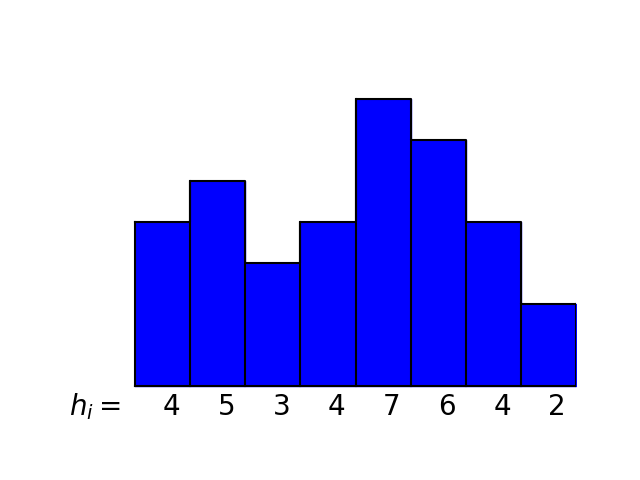
\includegraphics[width=0.9\linewidth]{int-dyn/sos-indiscernable.png}
    \end{minipage}
    \begin{minipage}[t]{0.5\linewidth}
        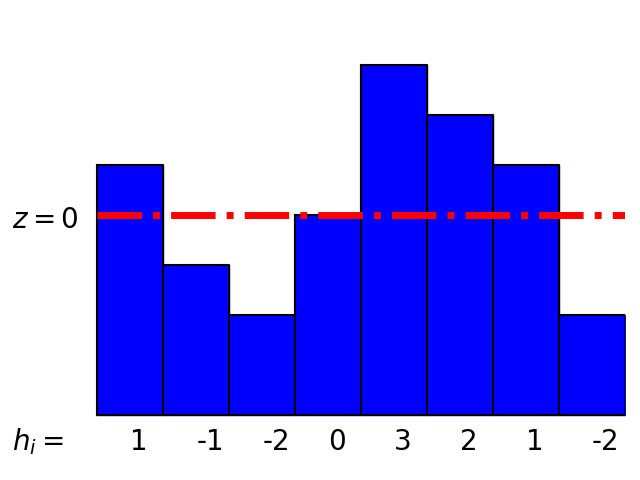
\includegraphics[width=0.9\linewidth]{int-dyn/sos-indiscernable-inf.png}        
    \end{minipage}    
    \caption{Possible configuration of the SOS model for a semi-infinite geometry (left) and infinite geometry (right). The red line shows the origin $z=0$. In the $i$-th column the interface is at height $h_i$. Particles under the interface are from the Ising $-$ phase, while particles over it are from the $+$ phase.}
    \label{figure-sos}
\end{figure}

Another way to compute this energy for a SOS configuration is to directly count the number of energy bonds for a $L'\times L$ Ising model under the approximation \eqref{approx-sos}. There are $L-1$ vertical bonds per column, where all have an energy of $-J$, while the link that goes though the interface has an energy of $+J$. The total contribution to energy from vertical bonds is thus 
\begin{equation}
    E_\perp = - J L' ( L-2)
\end{equation}
There are $L'\times L$ horizontal bonds. In a pure phase system, the horizontal energy would be $-JL'L$. Neverthelesss, there are $\sum_i |h_i-h_{i+1}|$ bonds which have an energy of $+J$, which gives the horizontal energy  contribution 
\begin{equation}
    E_\parallel = - J L' L + 2 \sum_i |h_i-h_{i+1}|
\end{equation}
By adding both, we find back Eq \eqref{energie-sos-ising}.

By setting $2J=J$ and getting rid of the bulk energy, we obtain the \textbf{Solid-On-Solid Hamiltonian} 
\begin{align}
H = J \sum_{i=0}^{L'} |h_i-h_{i+1}| + \frac{V(h_i)+V(h_{i+1})}{2}
\label{hamil-sos}
\end{align}



The first system where the SOS model has been applied was crystals' growth in 1972 \cite{gilmer_simulation_1972}. Since then, the model has been used with some success in naphthalene cristals\cite{elwenspoek_kinetic_1987}, experimental expitaxial growth\cite{wilby_scaling_1992}, polymer membranes \cite{boal_mechanics_nodate,gompper_steric_1989}, or interfacial wetting \cite{fisher_walks_1983}.

In the SOS model, the sites $i$ of height $h_i$ can take any value in $[0,L]$. The Restrictied Solid-On-Solid model (RSOS) is a variation where sites can only take the value $h_{i+1} \in [h_i-1,h_i,h_i+1]$\cite{privman_transfer-matrix_1989}. This approximation works for very low temperatures or very smooth interfaces \cite{kim_conserved_1994,vaysburd_critical_1995}. 

Another model, closer to the continuous model of Hamiltonian \eqref{heff} is the Discrete Gaussian model which has the following gaussian interaction
\begin{align}
H = J \sum_{i=0}^{L'} (h_i-h_{i+1})^2 + \frac{V(h_i)+V(h_{i+1})}{2}
\label{hamil-gsos}
\end{align} 
and also has a restricted version. The SOS model has an exact relation with the $XY$ model \cite{knops_exact_1977}, no matter the power law used for the interaction. With a generalization of this model to continuous heights, it has been shown that extreme deviations statistics of the interface is described by a scaling function \cite{schehr_universal_2006}. Since the energy costs of height differences $0,\pm 1$ are the same in every SOS model no matter the exponent  in the energy costs of height differences, one expects the qualitative freatures of all those models to be the same at low temperature, since height differences are typically small \cite{swendsen_monte_1977}.



Since the dimensionality of the system has been reduced in only taking into account the height interface $h_i$ at site $i$ instead of the position of all particles, we can think of an interface as a partially self-avoiding walk. This idea, which will be developed in section \ref{sec-continuous-model}, has proven quiet powerfull in finding exact solutions of the generating function \cite{owczarek_exact_1993} or the extreme deviations statistics of the interface \cite{majumdar_airy_2005,schehr_universal_2006}.

In the canonical ensemble, the height interface is fixed to $N$, which is translated in the partition function as
\begin{align}
Z(N) = \sum_{h_0 h_1 ... h_{L'}} \exp(- \beta \sum_{i} H(h_i,h_{i+1})) \delta_{\sum_i h_i, N}
\label{hamil-sos-cano}
\end{align}
In the grand-canonical ensemble, the conjugate variable to the height interface is the chemical potential $\mu$, and the grand partition function $\Xi$ is related to the canonical partition function by
\begin{align}
\Xi(\mu) =& \sum_N Z(N) \exp((\beta \mu N) \nn
=& \sum_{h_0 h_1 ... h_{L'}} \exp(-\beta H_{eff}(h_0,h_1,...,h_{L'})
\label{hamilk-sos-gce}
\end{align}
where
\begin{align}
H_{eff} = J \sum_{i=0}^{L'} |h_i-h_{i+1}|+ \sum_{i=0}^{L'} V(h_i)-\mu h_i
\end{align}
In Fig \ref{hauteur-mu}, we plot the mean number of particles per site with respect to the chemical potential, for different size of the system, in the thermodynamic limit $L' \to \infty$. When the chemical potential is too small, the Lagrange's multiplier of the mean height is negligible, allowing the interface to fluctuate freely. Since the height of the interface is then evenly spread over all possible configurations, the mean value for $\mu=0$ becomes $\frac{L}{2}$.


\begin{figure}
\centering
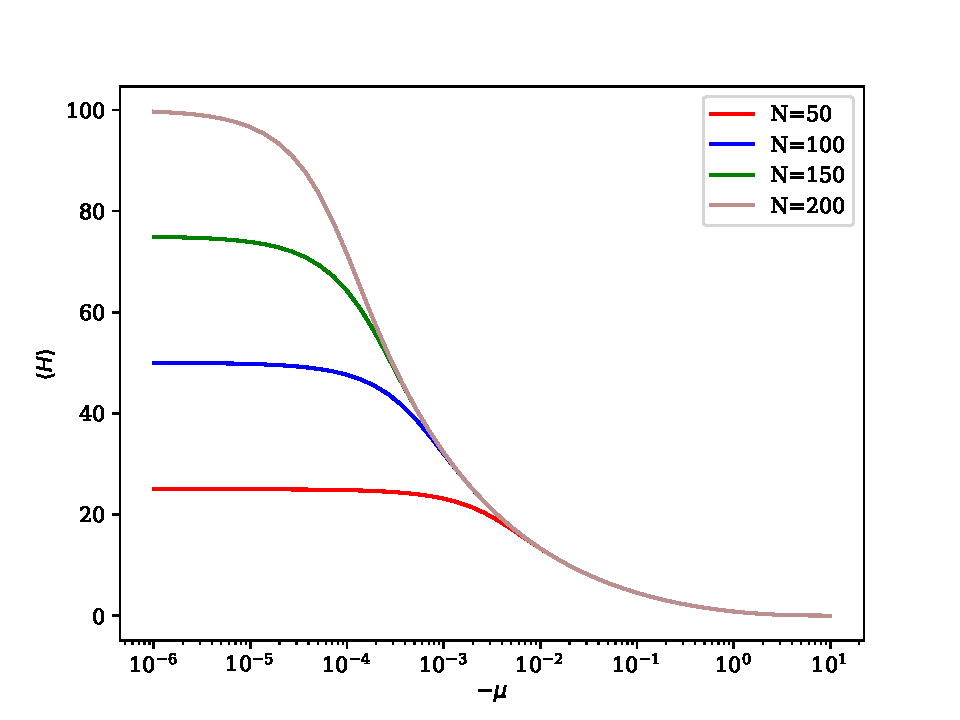
\includegraphics[width=0.7\linewidth]{int-dyn/hauteur-tm-sos.pdf}
\caption{Mean height of the SOS interface \eqref{hamilk-sos-gce} with respect to $- \mu$ through diagonalization of the transfer matrix for $\beta=1$, in the limit $L'\to \infty$. }
\label{hauteur-mu}
\end{figure}

%%%%%%%%%%%%%%%%%%%%%%%%%%%%%%%%%%%%%%%
\subsection{Transfer matrix}
%%%%%%%%%%%%%%%%%%%%%%%%%%%%%%%%%%%%%%%


In a more general fashion, we can rewrite the Hamiltonian as
\begin{align*}
H = \sum_{i=0}^{L'} f(h_i,h_{i+1}) + V(h_i,h_{i+1}) 
\end{align*}
where $f(h_i,h_j)$ is the energy interaction between two nearest neighbours and $V(h_i,h_j)=\frac{V(h_i)+V(h_j)}{2}$ is the external potential. We can rewrite the partition function as 
\begin{align}
Z = \sum_{h_1=0}^{L} \sum_{h_2=0}^{L}... \sum_{h_{L'}=0}^{L} \exp(- \beta \sum_{i=0}^{L'} H(h_i,h_{i+1}))
= \sum_{h_1 h_2 ... h_{L'}} \prod_{i=_0}^{L'} \exp(-\beta H(h_i,h_{i+1}))
\end{align}
We define the transfer matrix
\begin{align}
T(h_i,h_j) = e^{-\beta H(h_i,h_j)}
\label{matric-transfert}
\end{align}
In Fig \ref{mat-inf}, we have represented an infinite matrix corresponding the limit $L\to \infty$, where each site can take any value in $[-\infty,\infty]$. To diagonalize numerically such matrices, we translate the whole system with $h_i \to h_i - \frac{L}{2}$, where $L$ is the matrix's size, which me make tend to $\infty$.
The constraint \eqref{hamil-sos-cano} cannot be expressed in the transfer matrix formalism, which induces a change in properties from this ensemble with respect to the transfer matric results \cite{siegert_scaling_1993}.

Since the system has periodic boundary conditions $h_{L+1} = h_1$, we have $T(h_L,h_{L+1}) = T(h_L,h_1)$ \cite{pearce_exact_1989}. The matrix is thus symmetric, which means it can be diagonalized with eigenvectors and eigenvalues 
\begin{align}
T | \lambda> = \lambda |\lambda>
\end{align}
Those eigenvectors are orthonormal
\begin{align}
< \lambda | \lambda'> = \delta_{\lambda \lambda'}
\end{align}
We set $\lambda_0$ as the biggest eigenvalue of $T$, by $\lambda_1$ the second biggest eigenvalue, and so on. The partition function can then be rewritten, in terms of the transfer matrix \cite{abraham_transfer_1973} by
\begin{align}
Z = \sum_{h_1 h_2 ... h_{L'}} \prod_{i} T(h_i,h_{i+i}) = Tr( T^{L'}) = \sum_\lambda <\lambda | T^{L'} | \lambda> = \sum_\lambda \lambda^{L'}
\label{partition-trace-lambda}
\end{align}

\begin{figure}
\begin{align}
T = \begin{bmatrix} 
\ddots & \vdots & \reflectbox{$\ddots$} \\ 
e^{-\beta H(-1,-1)} & e^{-\beta H(-1,0)} & e^{-\beta H(1,-1)} \\
\dots & e^{-\beta H(0,0)} & \dots \\
e^{-\beta H(1,-1)} & e^{-\beta H(1,0)} & e^{-\beta H(1,1)} \\ 
\reflectbox{$\ddots$} & \vdots &\ddots \\ 
\end{bmatrix}
\end{align}
\caption{Infinite and symmetrical transfer matrix \ref{matric-transfert}.}
\label{mat-inf}
\end{figure}

In the thermodynamic limit $L' \to \infty$, only the biggest eigenvector is relevant since the partition function becomes
\begin{align}
Z(L\to \infty) \simeq \lambda_0^{L'}
\end{align}
We find that the free energy per site is 
\begin{align}
f = - \frac{1}{L' \beta} \ln(Z) \simeq - \frac{1}{\beta } \ln( \lambda_0)
\label{energie-libre-site}
\end{align}
In Fig \ref{fig-thermo-libre} we plot the evolution of the free energy per site $\Omega(L')$ without external field, compared to the thermodynamic limit. We determine that the thermodynamic limit becomes valid for $L' \greater 150 $.

\begin{figure}
\centering
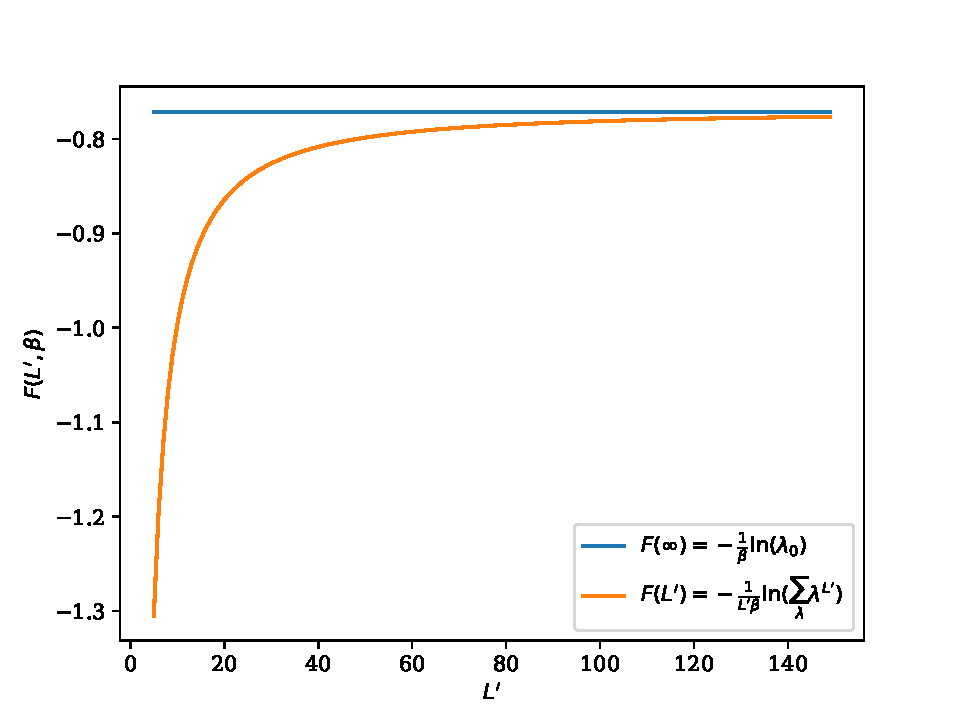
\includegraphics[width=0.7\linewidth]{int-dyn/freeene-thermo-libre.pdf}
\caption{Free energy per site $\Omega(L')$ with respect to the number of sites $L'$ compared to the thermodynamic value $\Omega(\infty)$, for a system of maximum height $L=100$, $\beta=1$, $J=1$ and $V(h_i)=0$.}
\label{fig-thermo-libre}
\vspace{-0.5cm}
\end{figure} 

To compute the mean height value per site $M$, we introduce the height matrix $\hat{M}$ defined by its action over the vectors $|h>$ in the matrix transfer's base by
\begin{align}
= \delta_{h,h'} h
\end{align}
We thus find that the density is
\begin{align}
M = < h > = \frac{1}{L'} \sum_i h_i = \frac{1}{Z} \sum_\lambda \lambda^{L'} < \lambda | \hat{M} | \lambda > \simeq < \lambda_0 | \hat{M} | \lambda_0 > 
\label{tm-magnetisation}
\end{align}
We deduce the mean displacement per site
\begin{align}
w^2 = < (h - M)^2 > = \frac{1}{Z} \sum_\lambda \lambda^{L'} < \lambda | \hat{M}^2 | \lambda > - < \lambda | \hat{M}| \lambda >^2 \simeq < \lambda_0 | \hat{M}^2 | \lambda_0 > - M^2
\end{align}
We can find thos two obersables by computing the first and second moment of the probability distribution that a site $i$ is at height $h_i$
\begin{align}
p(h) = \frac{1}{Z} \sum_\lambda \lambda^{L'} <\lambda | h >^2 \simeq < \lambda_0 | h >^2
\end{align}
The two-point correlation function of the system is computed by
\begin{align}
C(r) &= < h_i h_{i+r} > - M^2 = \frac{1}{Z} \sum_{\lambda \neq \lambda_0} < \lambda_0 | M | \lambda > < \lambda | M | \lambda_0 > \left( \frac{\lambda}{\lambda_0} \right)^r 
\end{align}
which becomes, in the long distance $r$ limit, 
\begin{align}
C(r) \simeq < \lambda_0 | M | \lambda_1 > < \lambda_1 | M | \lambda_0 > \left( \frac{\lambda_1}{\lambda_0} \right)^r
\end{align}
The correlation function has an exponential decay at large distances, which allows us to define the correlation length at large distance $\xi$
\begin{align}
\xi = - \frac{1}{\ln(\frac{\lambda_1}{\lambda_0})}
\label{longueur-correl-thermo}
\end{align}

%
%%%%%%%%%%%%%%%%%%%%%%%%%%%%%%%%%%%%%%
%	\subsection{États libres dans un système SOS infini}
%	\label{par-stab}
%%%%%%%%%%%%%%%%%%%%%%%%%%%%%%%%%%%%%%
%
%Prenons un système de taille $L$ dans la limite thermodynamique $L'\to \infty$. Comme vu précédement, seules les valeurs de la plus grand valeur propre influe sur les propriétés statistiques. Soit 
%\begin{align}
%    \psi_\lambda(h)= <h|\lambda>
%\end{align}
%la projection du vecteur propre associé à la valeur propre $\lambda$ de la matrice de transfert sur la base des hauteurs $|h>$ dans un système infini de part et d'autre de l'interface.
%Dans la limite $\beta=0$, c'est-à-dire pour une température infinie, tous les termes de la matrice de transfert sont égaux à $1$, menant à des vecteurs propres nuls. Dans ce cas, la densité de probabilité $p(h)$ est nulle pour tout $h$, ce qui signifie qu'il n'existe pas d'interface. Le modèle SOS n'est donc pas valable dans cette limite. De même, pour une température nulle $\beta=\infty$, la matrice de transfert devient la matrice identité. Les valeurs propres deviennent toutes égales à $1$ et les vecteurs propres sont $\psi_i(h) = \delta_{h,i}$ où ici $i$ est l'indice de la i-ème valeur propre $\lambda_i = 1$. La probabilité de trouver l'interface à la hauteur $h$ devient $p(h) = \frac{1}{Z}\sum_{i} <\lambda_i | h >^2 = 1$. La température nulle a pour effet de geler l'interface sur une seule hauteur, même si toutes les hauteurs sont équiprobables. Bien que les micro-états soient extrêmement différents pour une température finie, les propriétés macroscopiques sont identiques à cause du même poids statistique associé à chaque état.
%
%Pour une température finie et en absence de potentiel\cite{guyer_sine-gordon_1979,chui_pinning_1981}, l'équation du vecteur propre donne
%\begin{align}
%	\sum_{h=-\infty}^\infty T(h,h') \psi_\lambda(h) = \lambda \psi_\lambda(h')
%\end{align}
%En introduisant l'ansatz $\psi_\lambda(h) = \alpha_{\lambda}^h$ et en séparant de la somme les termes pour $h$ négatifs et positifs, on trouve aisément que 
%\begin{align}
%	\lambda = \frac{\sinh(\beta J)}{\cosh(\beta J)-(\alpha_{\lambda}+\alpha_{\lambda}^{-1})} 
%\end{align}
%Dans la limite thermodynamique, la probabilité de présence de l'interface à la hauteur $h$ est $p(h) = <\lambda_0|h>^2 = |\psi_0(h)|^2$. Le système ne possédant aucune brisure de symétrie particulière, la probabilité $p(h)$ est finie pour tout $h$ avec $p(h)=p(-h)$. Dès lors, l'ansatz supposé $\psi_\lambda(h) = \alpha_{\lambda}^h$ implique que $\alpha_{\lambda}$ soit de la forme $e^{ik}$ où $k$ est la longueur d'onde associée à la valeur propre $\lambda$. On obtient que 
%\begin{align}
%	\psi_k(h) =& e^{ikh} \\
%	\lambda =& \frac{\sinh(\beta J)}{\cosh(\beta J) - \cos(k)}
%	\label{lambda-sos}
%\end{align}
%
%L'existence d'une solution de ce genre indique que l'interface n'est pas localisée dans le cas d'un système infini (ou semi-infini) en absence de tout potentiel, ce qui conduit à de nombreux problèmes numériques. 
%
%Une manière simple de localiser l'interface est de rajouter un potentiel $V(h) = -B \delta_{h,0}$ \cite{chui_pinning_1999,chalker_pinning_1981,chalker_pinning_1982}, qui augmente la probabilité de présence de l'interface à $h=0$. La recherche d'un état localisé nous donne un ansatz de la forme 
%\begin{align}
%	\psi_\lambda(h) = \begin{cases} |\alpha|^h & \text{si } h \neq 0 \\ \psi_{\lambda,0} & \text{sinon} \end{cases} 
%\end{align}
%L'équation du vecteur propre devient
%\begin{align}
%	\sum_{h=-\infty}^\infty \exp(\beta |h-h'|- \beta B \delta_{h,0}) \psi_\lambda(h) = \lambda \psi_\lambda(h')
%\end{align}
%En notant $T(h,h') = R^{|h-h'|}$ pour $h \neq h' \neq 0$,  on obtient la même équation à un signe près dans l'exposant que l'on soit à $h'\greater 0$ ou $h' \greater 0$
%\begin{align}
%	\left( \frac{R}{\alpha} \right)^{\pm h'} \left[ \psi_{\lambda,0} + \frac{R \alpha}{1 - R \alpha} + \frac{\alpha}{R - \alpha} \right] + \left[ \frac{1}{1-R \alpha} - \frac{R}{R-\alpha} \right] = \lambda
%\end{align}
%Puisque cette équation est vraie pour tout $h'$, le premier terme doit être nul, ce qui nous donne
%\begin{align}
%	\psi_{\lambda,0} &= - \frac{\alpha}{R-\alpha}-\frac{R \alpha}{1-R \alpha} \\
%	\lambda &= \frac{1}{1-R \alpha} - \frac{R}{R-\alpha}
%\end{align}
%L'équation du vecteur propre à $h'=0$ nous donne par ailleurs 
%\begin{align}
%	\psi_{\lambda,0} + 2 \frac{R \alpha}{1-R \alpha} = \lambda \psi_{\lambda,0} e^{-\beta B}
%\end{align}
%L'existence d'une solution cohérente $\alpha \less 1$ autorise la présence d'une interface localisée grâce à un potentiel dit d'épinglage (\textit{pinning}) \cite{burkhardt_localisation-delocalisation_1981,kroll_solid--solid_1981,kroll_pinning_1982,kroll_interface_1983}.
%Dans le cas d'une géométrie semi-infinie, la présence d'un potentiel chimique exerçant une pression sur l'interface permet de la maintenir confinée, comme expliqué dans la section \ref{subsec-c-gc}.
%
%D'autres méthodes existent pour confiner l'interface. Le cisaillement d'une interface diminue sa largeur et permet de la localiser dans l'espace. On peut également proposer deux potentiels chimiques différents pour chaque phase à une hauteur de l'interface prédéfinie, comme le ferait un laser dans un liquie binaire dont chaque phase  a un incident de réfraction différent \cite{casner_laser-induced_2003,delville_laser_2009} (voir chapitre \ref{sec_laser}). Dans un système infini, une autre possibilité est de définir un champ magnétique symétrique rendant plus difficile la présence de l'interface loin de $0$. 


%%%%%%%%%%%%%%%%%%%%%%
    \section{Systems driven by imposed hydrodynamic flows}
%%%%%%%%%%%%%%%%%%%%%%

\begin{figure}
\centering
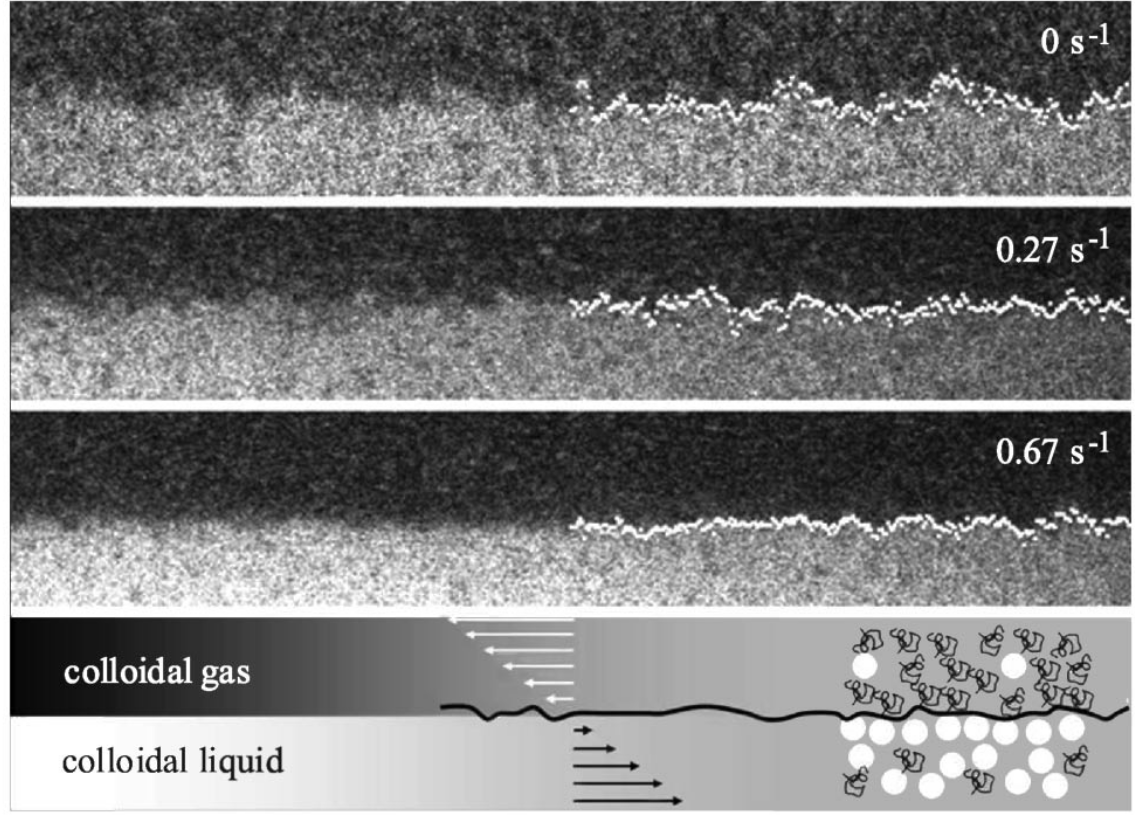
\includegraphics[width=0.7\linewidth]{int-dyn/derks.png}
\caption{Snapshot of the interface a sample of fluorescently labeled poly(methyl methacry-late) (PMMA) colloidal spheres in polystyrene close to the critical point, for different shear rates. The bottom panel schematically shows the flow geometry with the plane of zero velocity located at the interface. From \cite{derks_suppression_2006}. }
\label{snap-derks-shear}
\vspace*{\floatsep}
\begin{minipage}[t]{0.5\linewidth}
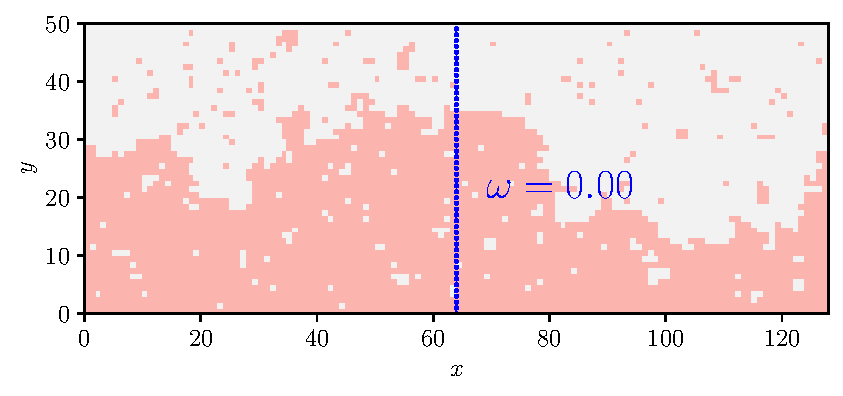
\includegraphics[width=\linewidth]{intro/cis-ising-f-000.pdf}
\end{minipage}%
\begin{minipage}[t]{0.5\linewidth}
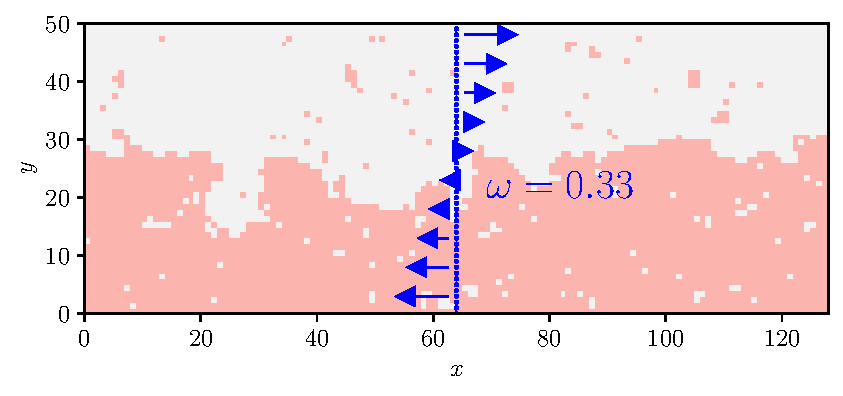
\includegraphics[width=\linewidth]{intro/cis-ising-f-033.pdf}
\end{minipage}
\centering
\begin{minipage}[t]{0.5\linewidth}
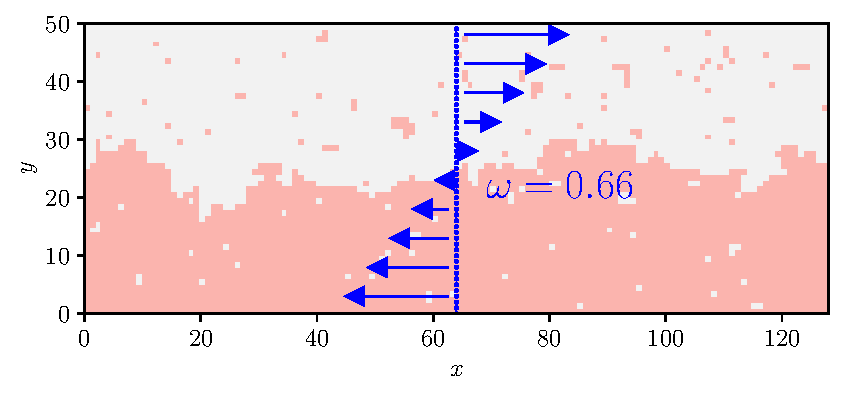
\includegraphics[width=\linewidth]{intro/cis-ising-f-066.pdf}
\end{minipage}
\caption{Snapshot of a 2D Ising model with respect to the shear \eqref{eq-cisaillement} with Kawasaki dynamics at $T=0.9 T_{2D,C}$.}
\label{snap-ising-shear} 
\end{figure} 

Here we consider what happens when a system is driven out of equilibrium. By driven we mean that energy is injected into the system by a laser \cite{girot_conical_2019}, by inducing a hydrodynamics flow, for instance a shear flow induced in a Couette cell in liquids \cite{derks_confocal_2004,derks_suppression_2006} or in glassy materials \cite{berthier_nonequilibrium_2002,berthier_shearing_2002}. In principle we should analyse this system with model H dynamics which couples diffusive model B dynamics to hydrodynamics in the low Reynolds number Stokes flow regime. In these dynamics the order parameter field will itself induce a hydrodynamics flow which will modify
the imposed one. However this full situation is very difficult to analyse and to a first approximation we can assume that the back reaction of the order parameter field on the hydrodynamic flow is small with respect to the imposed hydrodynamic flow and so we can simply write
\begin{equation}
\frac{\partial \phi (\bx,t)}{\partial t} + \nabla\cdot({\bf v}(\bx)\phi(\bx,t)) =- L\frac{\delta H}{\delta \phi(\bx)} + \eta(\bx,t),
\label{drive}
\end{equation}
where $L$ is given by the underlying model A or B dynamical operator and the noise has the correlation function as given by Eq. \eqref{gnoise}, and ${\bf v}(\bx)$ is the imposed (time independent) hydrodynamic flow or can equally well be an external drive imposed on the colloidal particles, due to the gravitational or electric field for example. 

The simplest case one can consider is where the driving field ${\bf v}(\bx) ={\bf v}_0$ is uniform \cite{leung_field_1986.bray_coarsening_2000}. Unfortunately this simple driving does not lead to a new steady state. Basically all of the colloidal particles acquire an average velocity ${\bf v_0}$ and so move along at the same speed relative to each other. Mathematically this can be seen by making the Galilean transformation
\begin{equation}
\phi (\bx,t)= \phi(\bx-{\bf v}_0t,t) = \phi({\bf y},t)
\end{equation}
This transformation eliminates the driving from the evolution equation \eqref{drive} and so we find an equilibrium system. 

The most studied example is where the driving is a shear flow \cite{derks_suppression_2006,thiebaud_nonequilibrium_2010}. The effective dynamics of the surface term in the presence of a shear flow, parallel to the interface \cite{bray_interface_2001,bray_interface_2001-1,}, is written as
\begin{equation}
{\bf v}(\bx) = \gamma z {\bf e}_x
\label{eq-cisaillement}
\end{equation}
and was studied using the method explained in section (\ref{heightd}). The addition of a shear flow leads to the appearance of a nonlinear term in $h$ and the interface statistics thus become non-Gaussian. In Fig \ref{snap-ising-shear} we show the influence of such a shear flow in numerical simulations, which is exactly the behaviour to be seen in capillary waves in polymer melts \cite{derks_confocal_2004,derks_suppression_2006}, see Fig \ref{snap-derks-shear} . The shear has a confining effect on the interface \cite{smith_driven_2010,smith_interfaces_2008-1,smith_interfaces_2008}, thus increasing the effective surface tension of the system.




%%%%%%%%%%%%%%%%%%%%
\section{Conclusion}
%%%%%%%%%%%%%%%%%%%% 

Statistical field theory \cite{bray_theory_1994} gives us a method to study the dynamics of equilibrium fields \cite{bellac_equilibrium_2004}. The surface tension of such a system is then defined as the difference of free energy between the bulk and the interface \cite{cahn_free_1958,abraham_transfer_1973}. The two main models are model A and model B \cite{hohenberg_theory_1977}, which decribe the dynamics of a field respectively in grand-canonical and the canonical ensemble. From those equations, we have defined what is an interface and have derived the Edwards-Wilkinson equation \cite{edwards_surface_1982} for both ensembles.
The Ising model \cite{niss_history_2005,niss_history_2006} provides a good way to study the bahviour of the field by discretization, which is easier to compute in numerical simulations \cite{newman_monte_1999}. The same kind of dimensional reduction can be done in order to get an interface lattice model which is called the Solid-On-Solid model \cite{gilmer_simulation_1972}. This model allows the use of the transfer method in an easier way than the Ising model\cite{privman_asymptotic_1989}. 
Also, the presence of out-of-equilibrum hydrodynamic flows tend to present interesting features. One such example is thee Couette shear \cite{derks_suppression_2006}, which has been found to smoothen the interface \cite{smith_interfaces_2008-1}.

\chapter{Numerical methods}
\label{chap-sim}

In 1949, Metropolis \cite{metropolis_monte_1949} discovers a method to compute, through Monte Carlo simulations, the expectation value of statistical quantities. If $Q$ is an observable quantity of a statistical system, such as the total energy or density of particles per site, then the expectation value is computed by weighting its value over all configurations $C$ with respect to their statistical weight. If we consider the system to be at thermodynamic equilibrium, then every configuration $C$ follows the Gibbs-Boltzmann distribution, and the mean value $<Q>$ is
\begin{align}
    <Q> = \frac{\sum_{C} Q(C) \exp(-\beta E(C))}{\sum_{C} \exp(-\beta E(C))}
\end{align}
For example, in a SOS system of size $100\times100$ - which is small compared to the thermodynamic limit as discussed in figure \ref{fig-thermo-libre} - there exist $100^{100}$ different possible configurations. In comparison, numerical simulations can explore up to $10^9$ configurations in a reasonable amount of CPU time.

Nevertheless, lattice models are well fitted for Monte Carlo simulations, where the goal is to compute is to compute such quantities. In the SOS model, all observables (and even quantities not observable such as the free energy) can be directly computed thanks to the matrix transfer in the grand-canonical ensemble. Nevertheless, as stated prior, the canonical ensemble stays out of reach of that method.

In this chapter, we start by explaining how Monte Carlo Metropolis algorithm works based upon the statistical ensemble we're interested in, at or out of equilibrium.
At last, I will give some technical considerations about optimizing numerical simulations.

This work has been made possible thanks to the Mésocentre de Calcul Intensif Aquitain (MCIA)\cite{noauthor_mesocentre_nodate}, where I've made the vast majority of the numerical simulations.
All the code I've produced can be found on Github \cite{paul_gersberg_github_2020} under Creative Commons BY 3.0 licence\footnote{\url{https://creativecommons.org/licenses/by/3.0/fr/deed.en}}. Numerical simulations where made with C++, parallelization with MPI, data treatment with Python, and some minor scripts in Bash.

%%%%%%%%%%%%%%%%%%%%%%%%%
    \section{Estimator}
%%%%%%%%%%%%%%%%%%%%%%%%%

Monte Carlo simulations explore the configurations' space in a random fashion \cite{newman_monte_1999} with a probability $p(C)$ which we will define later one. By choosing $M$ states ${C_0,...,C_M}$, the estimator $Q_M$ of $Q$ is given by
\begin{align}
    Q_M = \frac{\sum_{i=0}^M Q(C_i) p(C_i)^{-1} \exp(-\beta E(C_i))}{\sum_{i=0}^M  p(C_i)^{-1} \exp(-\beta E(C_i))}
\end{align}
The bigger the $M$, the better estimate the estimator provides for $<Q>$, up to the limit $Q_{M\to \infty} = <Q>$. If we select the configurations over which we sample the system according to the Gibbs-Boltzmann distribution $p(\nu) = Z^{-1} e^{-\beta E(C)}$, the estimator of $<Q>$ is
\begin{align}
    Q_M = \frac{1}{M} \sum_{i=0}^M Q(C_i)
\end{align}
The error over this estimate is
\begin{align}
	E(Q) = \sqrt{\frac{2 \tau}{M} (<Q^2>-<Q>^2)} 
\end{align}
This error does depend from the correlation time $\tau$ since if two states are really close in time, they would be strongly correlated, adding little information to the estimator. In practice, we just need $\frac{\tau}{M} \less 10^{-4}$ to obtain an error under $1\%$. This correlation time $\tau$ is computed through the autocorrelation function
\begin{align}
    \mC(t) = <Q(t')Q(t+t')>- <Q>^2 = \frac{1}{t}\int_0^t Q(t')Q(t+t')-<Q>^2 dt' 
\end{align}
which behaves as an exponential at long time\cite{wansleben_monte_1991}. A first order estimate of $\tau$ is thus given for
\begin{align}
	\tau = \int_0^{\infty} \mC(t)/\mC(0) dt
	\label{tau_cor}
\end{align}
Similarly, the measurement of the correlation length $\xi$ is given at first order by integration the two-point correlation function
\begin{align}
\mC(j) = \frac{1}{L'} \sum_{i=0}^{L'} <h_i h_{i+j}>-<h>^2 
\end{align}

%%%%%%%%%%%%%%%%%%%%%%%%%%%%%%
    \section{Monte Carlo Metropolis algorithm}
%%%%%%%%%%%%%%%%%%%%%%%%%%%%%%

We know want to know how to choose configurations, so all of them has the good equilibrium probability.

A dynamic for systems with a discrete configuration state can be built using Markov chains. Let the dynamic evolve in a discrete time $n$, and $p_n(C)$ the probability that the system is in configuration $C$ at time $n$. On the time step, if the system is in state $C$, it can jump to another state $C'$ with a transition probability $\rho(C\to C')$. The system at time $n+1$ thus only depends of the state at time $n$ : that's a Markovian process. The probability $p_{n+1}(C)$ to be in state $C$ at time $n+1$ is equal to the probability that the system was already in state $C$ at time $n$ and stays put with a transition probability $\rho(C\to C)$ , plus the probability that it was in state $C'$ and jumps towards $C$ with a transition probability $\rho(C'\to C)$. The master equation of such a dynamic is
\begin{align}
p_{n+1}(C) = \rho(C\to C) p_n(C) + \sum_{C'\neq C} \rho(C'\to C) p_n(C')
\end{align}
Since $\rho(C' \to C)$ is a probability, it meets the requirements 
\begin{align}
\sum_{C'} \rho(C' \to C) = 1
\label{norm}
\end{align}
Now, if the dynamics describes a system in interaction with a heat bath, the equilibrium distribution is given by
\begin{align}
p_{eq}(C) = \frac{\exp(-\beta E(C))}{Z}
\end{align}
with $Z$ the partition function. Since the equilibrium distribution is also stationary, we have
\begin{align}
p_{eq}(C) = \rho(C\to C) p_{eq}(C) + \sum_{C'\neq C} \rho(C'\to C)p_{eq}(C')
\label{p-eq-mc}
\end{align}
Another condition that we need in order to generate Gibbs-Boltmanzz states, is that it complies with detailed balance. To comply with detailed balance, the transition rate from a state to another one is equal to the rate from the reciprocal transition, which gives
\begin{align}
\sum_{C'} p(C) \rho(C \to C') = \sum_{C'} p(C') \rho(C' \to C)
\end{align}
We can show that this relation is equivalent to \cite{newman_monte_1999} 
\begin{align}
\frac{\rho(C'\to C)}{\rho(C \to C')} = \frac{p(C)}{p(C')} = \frac{\exp(-\beta E(C))}{\exp(-\beta E(C'))}
\end{align} 
By adopting the detailed balance, we easily see that the equilibrium distribution computed by Eq \eqref{p-eq-mc} gives back the Gibbs-Boltzmann distribution. 
During a Metropolis step, the transition probability of $C\to C'$ depends of the probability $g(C\to C')$ that this transition would be chosen amongst all the other possible transitions, and the acceptance rate $A(C \to C')$, which gives
\begin{align}
\rho(C\to C') = g(C\to C') A(C \to C')
\end{align}
For a lattice model site $L'$ sites, we say that a Monte Carlo time step is done when we have proceeded to $L'$ transition tries.
%%%%%%%%%%%%%%
\subsection{Glauber dynamics}
%%%%%%%%%%%%%%

In the SOS model with $L'$ sites of height comprised in $[0,L]$, the Glauber algorithm \cite{glauber_timedependent_1963} makes us chose a site $i$ at random with a uniform probability $\frac{1}{L'}$ and an integer $\alpha = \pm 1$ with probability $\frac{1}{2}$. If the configuration $C$ has the Hamiltonian $H(h_0,h_1...,h_i,...h_{L'})$, then the new generated configuration will have the Hamiltonian $H(h_0,h_1...,h_i+\alpha,...h_{L'})$.
If $\alpha=+1$, then we add a particle at site $i$, otherwise we remove one. In the case that $h_i+\alpha \not\in [0,L]$ , the generated configuration is not valid and discarded.
If the generated configuration is valid, the probability of selecting this transition is
\begin{align}
g(C\to C') = \frac{1}{2L'}
\end{align}
We thus have
\begin{align}
\frac{\rho(C\to C')}{\rho(C' \to C)} = \frac{A(C\to C')}{A(C'\to C)} = \exp(-\beta (E(C')-E(C'))
\end{align}
Is it possible to choose any acceptance rate $A(C\to C')$ which satisfies detailed balance. A Metropolis algorithm is an algorithm which has the following acceptance rate
\begin{align}
A(C\to C') = \begin{cases} \exp(-\beta (E(C')-E(C)) &\text{ si } E(C')-E(C) \greater 0 \\
1 &\text{ sinon} \end{cases}
\label{taux-transition-metropolis}
\end{align}
In practice, if $\Delta E \greater 0$, we randomly choose an integer uniformly in $r\in[0,1]$. If $r\less A(C\to C') $ then the transition is accepted. Otherwise, the transition is rejected and the system stays in the configuration $C$.

Since $\sum_i h_i$ is not conserved over time, Glauber dynamics corresponds to model A.

\begin{figure}
\centering
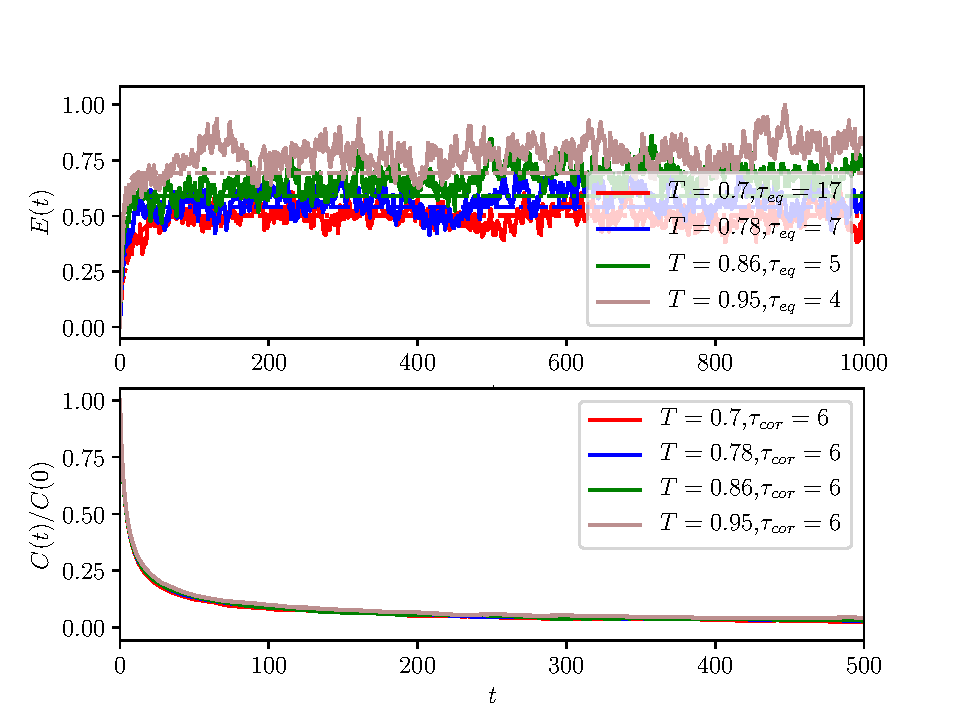
\includegraphics[scale=1]{numerical/sos-glau-eq-cor.pdf}
\caption{Plot of the energy per site (top) and the autocorrelation function (bottom) with Glauber dynamics from an initial state where $h_i=0$, for different temperatures.}
\label{eq-glau}
\includegraphics[scale=0.5]{example-image-a}
\caption{Mean height value per site with respect to $\mu$ different system size $L$ both by Glauber dynamics and diagonalization of the transfer matrix.}
\label{eq-glau} 
\end{figure}
The energy difference between two configurations is
\begin{align}
	\Delta E &= |h_{i-1}-(h_i + \alpha)| + |h_{i+1}-(h_i + \alpha)| - |h_{i-1}-h_i| - |h_{i+1}-h_i|  
\end{align}
It is not needed to compute the total height at each time step. We can stock $\sum_i h_i$ in a variable that is updated each time a transition is accepted by
\begin{align}
    <h>_{M+1} = <h>_M + \alpha
\end{align}
We can do the same for $\sum_i h_i^2$, which gives us the interface's width, or the total energy of the system with $\sum_i |h_i - h_{i+1}$.

In order to accelerate the equilibration process, we can directly start from the total height computed by the transfer matrix. We then get the equilibrium time by looking at $E(t)$. It is better practice to choose study the equilibration time by taking the total energy instead of the magnetization, since without external potential, the interface is delocalised and magnetization is only bounded by the boundary conditions. In Fig \ref{eq-glau}, we show the energy with respect to time and the autocorrelation function of the system in absence of chemical potential from a ground state $h_i=0$ for all $i$. The very small correlation and equilibration times means that numerical simulations reach the equilibrium distribution after $10^3$ MC steps, and that only $10^7$ MC steps will give accurate results.

In the SOS model, we expect to have the results from the Glauber dynamics to be exactly the same as the transfer matrix method, as shown in Fig \ref{tm-mc-equalt}, Since we can get exact results from the transfer matrix, the Glauber dynamics presents little interest for SOS models in the grand-canonical ensemble. Nevertheless, because there does not exist a transfer matrix formulation of the canonical ensemble, Monte Carlo simulations become interesting.

%%%%%%%%%%%%%%
\subsection{Kawasaki dynamics}
%%%%%%%%%%%%%%

Now we would like to have an algorithm for the canonical ensemble, where the total height stays constant. In the Kawasaki's algorithm \cite{kawasaki_diffusion_1966}, we randomly choose a site $i$ with probability $\frac{1}{L'}$, and one of its two neares neighboors $i-1$ or $i+1$ with probability $\frac{1}{2}$. For example, if we take the neighboor site $i-1$ (it holds the same for the site $i+1$), we generate a new configuration with Hamiltonian $H(h_0,...,h_{i-1}+1,h_i-1,...h_{L'})$, where we have taken a particle from site $i$ to diffuse it to the other site.
The selection probability is
\begin{align}
g(C\to C') = \frac{1}{2L'}
\end{align}
We also chose the same acceptance rate as in Glauber's dynamics \eqref{taux-transition-metropolis}.

Here, the total height is obviously conserved. In the case that we transfer a particle to site $i$ to site $i+1$, the energy difference is
\begin{align}
\Delta E &= |h_{i-1}-(h_i - 1)| + |h_{i+1} + 1 -(h_i- 1)| + |h_{i+1} + 1-(h_{i+2} )| \nn
& - \left( |h_{i-1}-h_i| + |h_{i+1} -h_i| + |h_{i+1}-h_{i+2}| \right)
\end{align}

\begin{figure}[t]
\centering
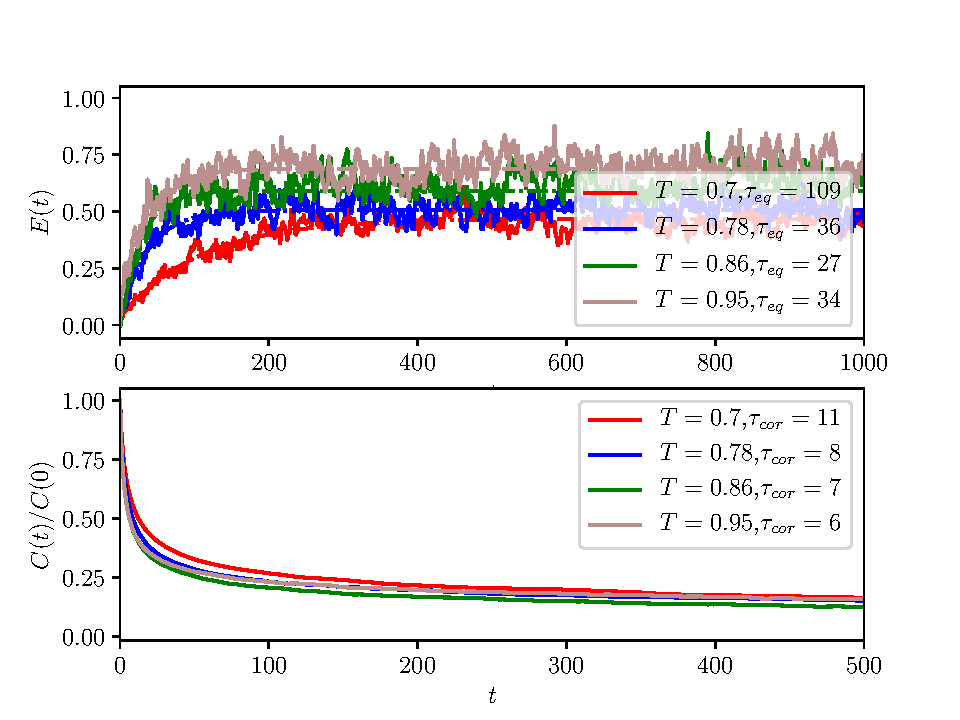
\includegraphics[scale=1]{numerical/sos-kaw-eq-cor.pdf}
\caption{Plot of the energy per site (top) and the autocorrelation function (bottom) with Kawasaki dynamics from an initial state where $h_i=0$, for different temperatures.}
\label{eq-kaw}
\end{figure}
In Fig \ref{eq-kaw}, we remark that both the equilibration and the correlation time are larger than for non-conserved dynamics, which is normal since the correlation length during coarsening goas as $t^\frac{1}{2}$ in model A and as $t^\frac{1}{3}$ in model B. Nevertheless they are of the same order of magnitude, which means that numerical simulations will take the same CPU time.

This dynamic describes the diffusion of particles at the interface. It is thus possible to add some hydrodynamic flow which breaks equilibrium. Since we have supposed that our configurations obeys the Gibbs-Boltzmann distribution, the Metropolis method stays pertinent if we assume that the dynamic is slow compared to the heat exchange with the reservoir.

%%%%%%%%%%%%%%%%%%% 
\section{Computing size dependent free energy}
%%%%%%%%%%%%%%%%%%% 

%%%%%%%%%%%%%%%%%%% 
\subsection{The Layer method}
%%%%%%%%%%%%%%%%%%%  

\begin{figure}
\begin{minipage}[t]{0.32\linewidth}
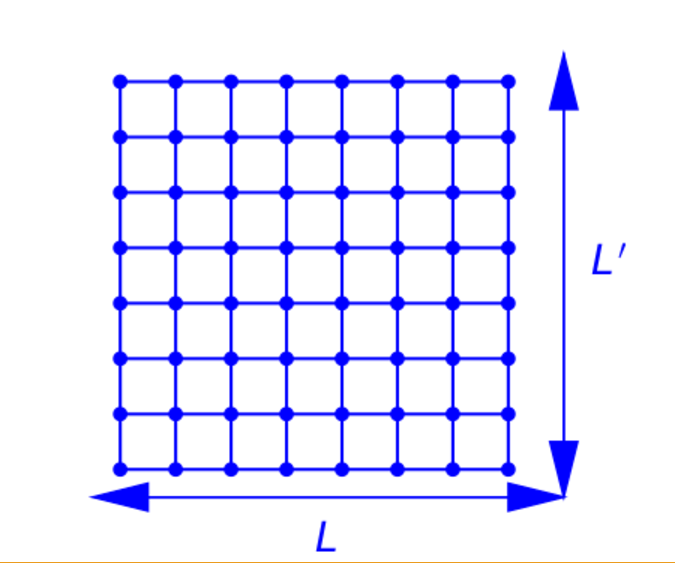
\includegraphics[width=\linewidth]{numerical/cross-h0.pdf}
\caption*{$H_0$}
\end{minipage}
\begin{minipage}[t]{0.32\linewidth}
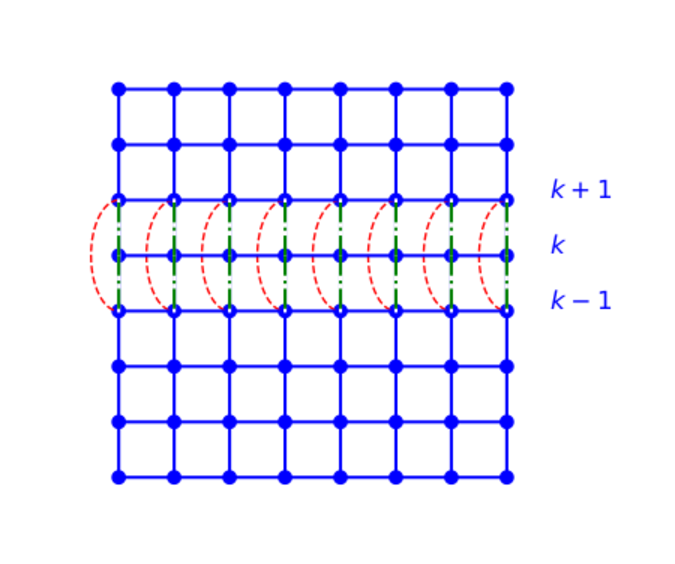
\includegraphics[width=\linewidth]{numerical/cross-hlambda.pdf}
\caption*{$H(\lambda)$} 
\end{minipage}
\centering
\begin{minipage}[t]{0.32\linewidth}
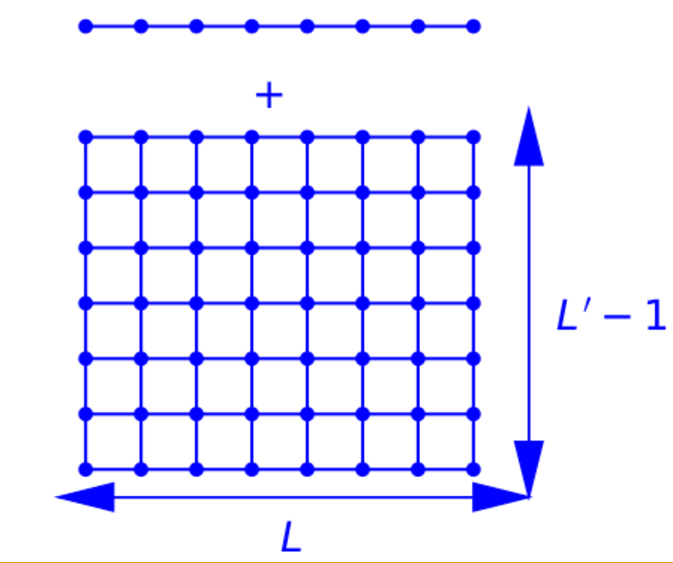
\includegraphics[width=\linewidth]{numerical/cross-h1.pdf}
\caption*{$H_1$}
\end{minipage}
\caption{Progessive decoupling of the $k$-th layer of the system in order to compute the freen energy through the Crossover Hamiltonian. Blue bonds have an energy of $\beta J$, red ones an energy of $\lambda \beta J $ and the green ones an energy of$ (1-\lambda) \beta J$. Reproduction 2D of \cite{ vasilyev_universal_2009}.}
\label{decouplage}
\end{figure}

It is not possible to compute from Monte Carlo simulations the free energy of a system, since it is not a derivative of the partition function. However, we can compute its derivative with respect to the system. This is useful to compute the Casimir force 
\begin{align}
F(t,h,L) = - \frac{\partial \Omega}{\partial L}
\label{casmir-mc}
\end{align}
To achieve that, Vasilyec \cite{vasilyev_universal_2009} developed a method to compute this derivative thanks to a dummy coupling parameter. Even though the system's size is discrete, it is possible to obtain a continuous-like size of the system thanks to the progressive decoupling the $k$-th layer of the system. If $H_0$ is the Hamiltonian of size $L$ and $H_1$ the Hamiltonian of size $L-1$ (see Fig \ref{decouplage}), then we define the crossover Hamiltonian as
\begin{align}
H_{cr}(\lambda) = (1-\lambda) H_0 + \lambda H_1
\label{hamil-trans}
\end{align}
with $\lambda \in [0,1]$, which interpolates from $H_0$ to $H_1$ when $\lambda$ goes from $0$ to $1$. As $\lambda$ goes on, we gradually decouple the $k$-th layer of the system, which means that the interaction energy of all vertical bonds between layer $k$ and layers $k-1$ and $k+1$ are now equal to $(1-\lambda)\beta J$, while we gradually couple the layers $k+1$ and $k-1$ with an energy $\lambda \beta J$.
The crossover Hamitlonian $H_{tr}(\lambda)$ also depends from the position of the decoupled layer $k \in {1,2,...,L}$ . The free energy associated to this system is
\begin{align}
\Omega_{cr}(\lambda) = -k_B T \ln \left( \sum_{h_1 ... h_L} \exp(-\beta H_{tr}(\lambda)) \right)
\end{align}
From the derivative of the free energy with respect to $\lambda$, we find
\begin{align}
\frac{\Omega_{cr}(\lambda)}{d\lambda} = < H_1 - H_0>_{H_{cr}(\lambda)}
\end{align}
where $< \cdot >_{H_{cr}(\lambda)}$ represents the statistical mean value in the crossover system, easily computable in numerical simulations. By integrating over the coupling constant, we have
\begin{align}
\Omega_1 - \Omega_0 = \int_0^1 d\lambda < H_1 - H_0>_{H_{cr}(\lambda)}
\end{align}
Finally, in the thick limit where $L\gg1$, we find
\begin{align}
- \frac{\partial \Omega(t,h,L)}{\partial L} \simeq \int_0^1 d\lambda < H_1 - H_0>_{H_{cr}(\lambda)}
\end{align}
Even though $H_{cr}(\lambda)$ depends of which layer we decided to decouple, and by transition $H_1-H_0$ and $< H_1 - H_0>_{H_{cr}(\lambda)}$, the integrand $\int_0^1 d\lambda < H_1 - H_0>_{H_{tr}(\lambda)}$ should be independent of this choice, as long as boundary conditions are not affect by the $k$-th layer.

For the SOS model, it is possible to exactly compute the energy variation produced by the decoupling. We find that
\begin{align}
&H_{cr,SOS}(\lambda) = H_{0,SOS} - \nn
&\frac{\lambda J}{2} \sum_x \left[ \sgn(k-1-h(x)) \sgn(k+1-h(x)) - \sgn(k-h(x)) \left( \sgn(k-1-h(x))+\sgn(k+1-h(x)) \right) \right]
\end{align}
where the prefactor $\frac{1}{2}$ take into account the prefactor between Ising and SOS models in Hamiltonian \eqref{energie-sos-ising}. By doing the ?? {\color{red} how do you translate "tableau de valeurs" ? } , we notice that every term in the sum is equal to $-1$ independently of $k$, since contrary to Ising models, SOS models do not possess any bulk energy. We 

%%%%%%%%%%%%%%%%%%% 
\subsection{The Lopes Cardozo method}
%%%%%%%%%%%%%%%%%%% 
Since the Layer method does not work for our models, we have to look to other ways. In the case of a chemical potential conjugated with the total height, we see that \cite{lopes_cardozo_critical_2014}
\begin{align}
<\sum_i h_i>(\mu,L) = - \frac{\delta \Omega(\mu,L)}{\delta \mu}
\end{align} 
If we integrate over the chemical potential, we have
\begin{align}
\Delta \Omega(\mu_1,\mu_2) = \Omega(\mu_1,L) - \Omega(\mu_2,L) = - \int_{\mu_1}^{\mu_2} <\sum_i h_i>(\mu,L) dh
\label{integration-cardozo}
\end{align}
In the case where we know the analytical forme of the free energy in the limits $\mu_2 \to \infty$ or $\mu_1 \to 0$, this method provides a way to directly measure the free energy of the system for any temperature or size by integrating over the chemical potential.

In the limit $\mu_2 \to \infty$, the correlation length at the reference state will be small so that the reference free energy will be essentially that of the bulk. As a consequence, it should contain all the information of the Casimir force \eqref{casmir-mc}. That derivative force can then be computed by 
\begin{align}
\delta L \frac{\partial \Omega(\mu_1,L)}{\partial L} = \Delta \Omega(\mu_1,\mu_2,L)-\Delta \Omega(\mu_1,\mu_2,L-\delta L)
\end{align}
where $\delta L$ is the difference thickness between two systems, and which is then independent of $\mu_2$ in the large chemical potential limit as the free energy $\Omega(\mu_2,L)$ converges to the bulk energy.

Since in Kawasaki dynamics the total height is constant, this method does work only for model A.

%%%%%%%%%%%%%%%%%%% 
\section{Tips and tricks}
%%%%%%%%%%%%%%%%%%% 

The simulation's speed of SOS models is so great compared to Ising ones that it is possible to study systems over a wider range of parameters. A SOS simulation of $10^7$ MC steps takes roughly 20 minutes to complete once fully optimized. We see that if we want to launch hundreds of those simulations, it can easily take days, which forces us to optimize the code.
In C++, if compiling with g++, the first thing to do is to compile the programme with the $-O3$ flag, which makes you gain an order of magnitude in CPU time.

The most important part of Monte Carlo simulations are the pseudo Random Number Generator (pRNG), which are called at least twice for each transition attempt. The C++ standard library proposes the function \textit{default\_random\_engine} as the default pRNG. A lot of CPU time can be saved by switching to \textit{sfc64} or \textit{xoroshiro} pRNGs. Furthemore, the generation of $\pm1$ numbers only require one bit, while the pRNG always generates a 64-bits number, thus wasting 63-bits at each boolean generation. A wasteless method which speeds considerably the simulation's speed can be found in \cite{martin_ankerl_fast_nodate}.

Lastly, the easiest way to gain real time is to make the code parallel. We can do that either by domain decomposition - which would allow us to simulate larger systems - or parallelise directly over the simulation's parameters (as the temperature or the chemical potential). While the first one is useless in SOS model because of the short correlation length of such systems, the latter can be done via two libraries : OpenMP and MPI. It took me some time to understand that the memory-shared OpenMP protocol has a lot of problems with pRNGs, making this library not suited for Monte Carlo simulations. On the contrary, the MPI library provides impermeability between threads, which makes it the better choice.

%%%%%%%%%%%%%%%%%%%%%%%%%%%%%%%%%%
\section{Conclusion}
%%%%%%%%%%%%%%%%%%%%%%%%%%%%%%%%%%

In this chapter, we have explained how to compute expectation values of observables in our system, thanks to the Monte Carlo Metropolis algorithm. For that, we need to suppose that the system is in thermal equilibrium with a heat bath, and that it respects detailed balance. We have two different possible algorithms : the Glauber dynamics allows to study the systems in the grand-canonical ensemble, while the Kawasaki dynamics is for canonical ones. Nevertheless, since the transfer matrix method gives exact results for the grand-canonical ensemble, only the Kawasaki dynamics is relevant for SOS models. 

In addition to that, measuring the free energy of the system is not an easy task, as we can only compute its derivative. The first method we have presented is about progressively decoupling a layer of the system, even though for SOS models, which do not possess a bulk energy, the method does not work. Another method is to integrate over the conjugate variable coupled to the total height, which is the chemical potential. This method does not work for Kawasaki algorithms. 
Since as we have discussed Glauber simulations are not relevant for our models, we find that we have no way to compute the free energy in Monte Carlo methods for the only relevant ensemble which is the canonical one. In a latter chapter, we will see how to fix this issue.
%%%%%%%%%%%%%%%%%%%%
\chapter{Equilibrium Interface models and their finite size effects}
%%%%%%%%%%%%%%%%%%%%

Models for interfaces arise naturally in phase separated systems, as explained in \ref{chap-int-dyn}. Finite size corrections are manifested when the correlation length becomes of the order of magnitude of the system's size. When undergoing a continuous phase separation, the system exhibits finite size corrections which are manifested by a long range critical Casimir interaction, which we describe in the first section. In the second section we examine finite size effects in continuous interface models in one dimension, and show that while they have similar long-range interactions, the forces induced by interface confinement are quite different, and will be compared to the GSOS model. In the last section, we compute the size-dependent eigenvalues of the transfer matrix for the free SOS model, and compare the results with previous works.

%%%%%%%%%%%%%%%%%%%%
\section{The Casimir effect}
\label{sec-casimir}
%%%%%%%%%%%%%%%%%%%%

Here we explain the critical Casimir effect. For completeness we start by explaining the quantum Casimir effect as it was in the quantum context that the effect was first observed \cite{h_b_g_casimir_attraction_1948}.
We also describe the basis of the Lifshitz theory that generalises Casimir's contribution to 
general dielectric materials beyond the perfectly conducting plate paradigm.

%%%%%%%%%%%%%%%%%%%% 
\subsection{Quantum Casimir effect}
%%%%%%%%%%%%%%%%%%%%
In an ideal conductor, the free charges can move arbitrarily quickly to cancel out any electric in the plane \cite{richard_feynman_feynman_1963}. Thus, a perfectly conducting plate in the $(x,y)$ plane imposes boundary conditions on the electromagnetic field
\begin{equation}
{\bf E}\times {\bf n} = {\bf 0};\ {\bf B}\cdot {\bf n} = 0
\end{equation}
The quantum Hamiltonian for the electromagnetic field is given by 
\begin{equation}
H = \sum_{\bk,\lambda}\hbar \omega(\bk,\lambda)\left[a^\dagger(\bk,\lambda)a(\bk,\lambda) + {1\over 2}\right]
\end{equation}
Here $\lambda$ denotes the polarisation (there are two polarisation states) and $\bk$ the wave vector. The dispersion 
relation for photons is
\begin{equation}
\omega(\bk,\lambda) = |\bk|c.
\end{equation}
The ground state energy of the electromagnetic field \cite{h_b_g_casimir_attraction_1948} is given by
\begin{equation}
E_0 = < 0|H|0> = H = \sum_{\bk,\lambda}{1\over 2}\hbar \omega(\bk,\lambda)= \sum_\bk\hbar |\bk|c
\end{equation}

The presence of conduction plates at $z=0$ and $z=L$ means that the wave vectors $k_z$
must be quantised according to $k_z= n\pi/L$ where $n \in \{0,\ 1, \ 2, \ \cdots\}$ while
if the $(x,y)$ plane has a large area $A$ we can write
\begin{equation}
\sum_{k_x,k_y}\ \cdot= {A\over (2\pi)^2}\int d^2\bk \ \cdot
\end{equation}
This then gives 
\begin{eqnarray}
E_0(L) &=& {\hbar c A\over (2\pi)^2}\sum_{n=0}^\infty \int d^2\bk \left(\bk^2 + {n^2\pi^2\over L^2}\right)^{1\over 2} \\
&=& {\hbar c A\over (2\pi)}\sum_{n=0}^\infty \int_0^\infty kdk \left(\bk^2 + {n^2\pi^2\over L^2}\right)^{1\over 2}
\end{eqnarray}
The problem with the above expression is that it is clearly divergent. However it can be rendered finite by cutting off the high momentum degrees of freedom by writing
\begin{equation}
E_0(L) = {\hbar c A\over (2\pi)}\sum_{n=0}^\infty \int_0^\infty kdk \left(\bk^2 + {n^2\pi^2\over L^2}\right)^{1\over 2} f\left((\bk^2 + {n^2\pi^2\over L^2})^{1\over 2}\right)
\end{equation}
where $f$ is a smooth function such that $f(p)=1$ for $p\ll\Lambda$ and $f(p)=0$ for $p\gg\Lambda$. Here, $\Lambda$ is an ultraviolet cut-off and $f$ thus only counts the contribution of photons with a momentum less than $\hbar\Lambda$. For this sort of calculation to make physical sense the physical result we get at the end should be independent of both the choice of $f$ and $\Lambda$. 




In the limit $L\to\infty$ we can replace the sum over discrete modes by an integral, as usual in statistical physics, 
\begin{equation}
E_0(L) = {\hbar c A\over (2\pi)}\int_{0}^\infty {L\over \pi}d\nu \int_0^\infty kdk \left(\bk^2 + \nu^2\right)^{1\over 2}f\left((\bk^2 + \nu^2)^{1\over 2}\right)
\end{equation}
where we have used $d\nu = \pi/L$. We thus see that for large $L$ we have
\begin{equation}
E_0(L) = AL \epsilon_{bulk}
\end{equation}
where $\epsilon_{bulk}$ is a bulk energy density per unit of volume, that is to say the total energy is extensive.  The computation above only calculates the energy of the EM field between the plates. If the physical system extends up to $L'\gg L$, then the total energy of {\color{red} both the interior and the exterior of the plates} is
given by
\begin{equation}
E_{total}(L) = E_0(L) + A(L'-L)\epsilon_{bulk}
\end{equation}
We see that the part of the energy that depends on $L$ is given by
\begin{equation}
U(L) = E_0(L)- AL\epsilon_{bulk}
\end{equation}
It is the derivative of $U$ which gives the physical interaction between the two plates, the pressure associated with this interaction in the colloid science literature is called the disjoining pressure \cite{stubenrauch_disjoining_2003} where to compute the effective interaction the bulk pressure has to be subtracted.
Now we simply write 
\begin{equation}
AL\epsilon_{bulk} = {\hbar c A\over (2\pi)}\int_{0}^\infty dn \int_0^\infty kdk \left(\bk^2 + {n^2\pi^2\over L^2}\right)^{1\over 2} f\left((\bk^2 + {n^2\pi^2\over L^2})^{1\over 2}\right)
\end{equation}
where we have put the $L$ dependence in the integral. This then gives
\begin{equation}
U(L) = {\hbar c A\over (2\pi)}\left[\sum_{n=0}^\infty g(n) -\int_0^\infty dn \ g(n)\right]
\end{equation}

where
\begin{equation}
g(n) = \int_0^\infty kdk \left(\bk^2 + {n^2\pi^2\over L^2}\right)^{1\over 2} f\left((\bk^2 + {n^2\pi^2\over L^2})^{1\over 2}\right) = {1\over 2}\int_{n^2\pi^2\over L^2}^\infty du u^{1\over 2} f(u^{1\over 2})
\end{equation}
We now use the Euler-Mauclarin formula
\begin{equation}
\sum_{n=0}^\infty g(n) -\int_0^\infty dn \ g(n) = -B_1g(0) -{1\over 2} B_2 g'(0) - {1\over 24} B_4 g'''(0) - \cdots
\end{equation}
where $B_n$ are the Bernoulli numbers\footnote{The first Bernoulli numbers are explicitly given by $B_1 =1\ , B_2 = {1\over 2} ,\ B_4 = -{1\over 30}$}.
We find that
\begin{equation}
g'(n) = -{\pi^3\over L^3} n^2 f({n\pi\over L})
\end{equation}
and noticing than in the region around $n=0$, $f=1$ is a constant, we show that
\begin{eqnarray}
g'(0) &=& 0 \\
g''(0) &=& 0 \\
g'''(0) &=& -{2\pi^3\over L^3}
\end{eqnarray}
Higher order derivatives are zero so the full result is given by the first three terms of the Euler-Maclaurin formula. We thus find
\begin{equation}
U(L) = {\hbar c A\over (2\pi)}\left[ -g(0) -{\pi^3\over 360 L^3}\right]
\end{equation}
The first term independent of $L$ can be interpreted as a surface energy. The effective $L$ dependent interaction is given by
\begin{equation}
U_{int}(L) = -{\hbar \pi^2 c A\over 720 L^3}
\end{equation}
We see that the effective interaction is attractive. Interestingly Casimir thought that his calculation could explain the stability of the electron \cite{h_b_g_casimir_attraction_1948,carazza_casimir_1986} The model of the electron is one of a perfectly conducting shell carrying an electric charge $e$. If the radius of the shell is $a$ then the electrostatic energy of due to the charge is given by
\begin{equation}
E_{Charge} = {e^2\over 8\pi a\epsilon_0}
\end{equation}
There is thus a repulsive force on the shell which should make it expand. Casimir thought that the Casimir force on a spherical geometry, 
if is an attractive force as is the case for the parallel plate geometry, could stabilise the electron. Clearly by dimensional analysis
\begin{equation}
E_{Cas} = -{Z\hbar c\over a}
\end{equation}
The balance of the Casimir and electric forces would then require
\begin{equation}
Z = {e^2\over 8\pi \hbar c}.
\end{equation}
However, in the case of conducting spherical shell, the constant $Z \simeq -0.046175$ is negative \cite{boyer_quantum_1968,milton_casimir_1978,bowers_casimir_1998}, while the same calculation for a cylindrical geometry predicts an attractive force \cite{milton_casimir_1978-1}. 

%%%%%%%%%%%%%%%%%%%%
\subsection{Lifshitz Theory}
%%%%%%%%%%%%%%%%%%%%
{\color{red} I've retouched some phrases and removed the names, instead just citing the papers, since I feel you've said the names so I could find the papers. }
The Casimir calculation is based on the boundary conditions imposed on the EM field 
due to a conductor. However, this is an ideal mathematical limit, conductors being conductors because free charges can move to cancel out the electric field in the conducting surface.
The Casimir force can also be seen as due to correlations induced in the charge fluctuations in each plate, which allows for an alternative method based on sources which recovers the Casimir force \cite{julian_schwinger_casimir_1978,schwinger_casimir_1992}. In a sense therefore the effect can be interpreted without reference to the zero point energy of the vacuum and the Casimir calculation works due to the fact that the mathematical limit in going to a perfect conductor works. 
Using a stochastic formulation of electrodynamics by Rytov \cite{sm_rytov_principles_1989}, the Casimir calculation was generalized by Lifshitz for interactions between arbitrary electrical bodies, characterized by their local electric and magnetic response\cite{lifshits_theory_1955}. 
Even though this theory is very general, the microscopic justification is not completely rigorous, source terms (random currents and dipole fluctuations) are introduced to Maxwell's equations to give a Langevin formulation of Maxwell's equations in the presence of dielectric bodies. The correlation functions of the white noise terms depend on the temperature of the system and are determined via the quantum fluctuation dissipation theorem. The Lifshitz theory is computationally difficult to work with and it was reformulated in a way more useful for practical calculations and that can be applied to experimental setups \cite{van_kampen_macroscopic_1968,ninham_van_1970}.
Rytov's formulation has the advantage that it can be used to treat out of equilibrium situations where different bodies at held at different temperatures interact. This allows both the computation of out of equilibrium forces and radiative heat transfer. 

The theory in the presence of electromagnetic media is written in terms of the electric and magnetic fields ${\bf E}$ and ${\bf B}$ and the displacement and magnetizing fields ${\bf D}$ and ${\bf H}$ which are assumed to obey local relations in real space and Fourier space
\begin{equation}
\tilde {\bf D}(\omega)=\epsilon(\omega)\tilde{\bf E}(\omega); \ \tilde {\bf B}(\omega)= \mu(\omega) \tilde{\bf H}(\omega)
\end{equation}
where $\tilde\epsilon( \omega)$ and $\tilde\mu( \omega)$ are the frequency dependent
permittivity and permeability. The boundary conditions at the interface between two materials $1$ and $2$ are given by
\begin{eqnarray}
B_{1n}= B_{2n} && \ D_{1n}=D_{2n} \\
E_{1t} = E_{2t} && \ H_{1t}=H_{2t}
\end{eqnarray}
where $n$ denotes the normal component and $t$ the tangential component to the interface.

Forces can be computed using the vacuum (assuming that the surface where the force is computed is next to the vacuum) Maxwell stress tensor.
\begin{equation}
T_{ij}= \epsilon\left(E_iE_j -{1\over 2}\delta_{ij}E^2\right) + {1\over \mu}\left( B_i B_j -{1\over 2}\delta_{ij}B^2\right)
\end{equation}
Notice that the stress tensor is quadratic in the fields ${\bf E}$ and ${\bf B}$, this means that even if the fields are on average zero, both thermal and quantum fluctuations give rise to forces.

In media Maxwells equations are
\begin{eqnarray}
\nabla \times{\bf E} &=& -{\partial {\bf B}\over \partial t} \\
\nabla \times{\bf H} &=& {\bf J}-{\partial {\bf D}\over \partial t} \\
\nabla \cdot {\bf D} &=& \rho\\
\nabla \cdot {\bf B} &=& 0 
\end{eqnarray}

In a dielectric medium or conductor where there are no applied external fields there is no free charge or current . As such, the average values of ${\bf E}$ and ${\bf B}$ are zero. Rytov's idea was to add a random current to induce both thermal and quantum fluctuations
into the problem. If we assume that the only contribution to the current comes from a fluctuating polarization density ${\bf P}$ we can write
\begin{equation}
{\partial \rho\over \partial t} +\nabla \cdot {\bf J}= 0\implies\nabla\cdot \left[-{\partial {\bf P}\over \partial t} +{\bf J}\right] = 0
\end{equation}
where we have used
\begin{equation}
\rho = -\nabla \cdot {\bf P}
\end{equation}
This means that the current is given by
\begin{equation}
{\bf J}={\partial {\bf P}\over \partial t} 
\end{equation}
or in Fourier space
\begin{equation}
\tilde {\bf J}(\omega)= i\omega \tilde P(\omega)
\end{equation}
Now if we assume that the fluctuations in the polarization density are uncorrelated in space, the fluctuation dissipation theorem tells us that the correlation function of the polarization density in Fourier space is given by
\begin{equation}
< P_\alpha(\omega; \bx)P^{\dagger}_\beta(\omega; \bx')>_{sym}=
{\hbar \epsilon''(\omega)\over 2}\coth\left({\hbar\omega\over 2k_B T}\right)\delta(\omega-\omega')\delta(\bx-\bx')\delta_{\alpha\beta}
\end{equation}

\begin{equation}
\epsilon(\omega) = \epsilon'(\omega)+i\epsilon''(\omega)
\end{equation}
The Lifshitz calculation for slab geometries gives a force per unit area between two slabs of media separated by a distance $L$
\begin{eqnarray}
{F\over A} &=& -{k_BT \over \pi c^3}\sum_{n=0}^\infty \omega_n^3 \int_1^\infty dp p^2 \ 
\left[ 1-{(s_1+p)(s_2+p)\over (s_1-p)(s_2-p)}\exp(-{2p\omega_n L\over c})\right]\nonumber \\
&+&\left[ 1-{(s_1+p\varepsilon_1)(s_2+p\varepsilon_2)\over (s_1-p\varepsilon_1)(s_2-p\varepsilon_2)}\exp(-{2p\omega_n L\over c})\right]
\end{eqnarray}
where $\epsilon = \epsilon_0\varepsilon$, $s_i = \sqrt{\epsilon_i -1 +p^2}$,
$\omega = {2\pi nk_BT \over \hbar}$ are the Mastubara frequencies \cite{matsubara_new_1955} and ${\varepsilon_i
=\varepsilon_i(i\omega_n)}$. Note that the integral over real frequencies has become a sum over discrete Matsubara frequencies, they come from the poles in the hyperbolic cotangent.

One needs to know the dielectric response at imaginary frequency, this is done using the Kramers-Kronig relation
\begin{equation}
\varepsilon(i\omega)= 1 +{2\over \pi}\int_0^\infty d\zeta {\zeta \varepsilon''(\zeta)\over \omega^2 + \zeta^2}
\end{equation}


%%%%%%%%%%%%%%%%%%%%
\subsection{Critical Casimir effect}
%%%%%%%%%%%%%%%%%%%%

{\color{red}
In systems having a continuous phase transition the correlation length diverges as the critical point is approached. This means that the correlation length has a size comparable to that of the system size, this  leads to strong finite-size effects in the free energy. Following the arguments of Fisher and de Gennes \cite{gambassi_casimir_2009}, we describe how a version of  the Casimir effect is manifested in  critical systems. 
}
%%%%%%%%%%%%%%%%%%%%
\subsubsection{Bulk scaling for near critical systems}
%%%%%%%%%%%%%%%%%%%%
The free energy for a system consisting of $N$ spins has a singular part at a critical temperature $T_c$ which can be written as
\begin{equation}
F(t,h) = N f(t,h)
\end{equation}
where $t = (T-T_c)/ T_c$ measures the distance from the critical point and $h$ is the external applied magnetic field. We assume that we are in a system where the only relevant parameters are $T$ and $h$ (equivalently the concentration or chemical potential of a binary mixture), which is true for $d\less 4$ \cite{amit_field_2005}.
Now if we carry out a renormalisation group transformation
blocking spins in blocks of linear size $b$ into new effective spins, the RG transformation
gives
\begin{equation}
N f(t,h) = N'f(t',h')
\end{equation}
Clearly the number of spins in the blocked system is given by $b^d N'=N$ and the RG transformation for $t$ and $h$ are given by $t' = b^{y_1} t$ and $h' = b^{y_2}h$, where $y_1$ and $y_2$ are positive and are the RG exponents for the fields $t$ and $h$ (from which all critical exponents can be deduced). This then means that
\begin{equation}
f(t,h) = {1\over b^d}f(b^{y_1} t, b^{y_2} h) 
\label{rg}
\end{equation}
We begin by working with $t\greater 0$ but the arguments here are trivially generalisable to the case $t\less 0$. In Eq. (\ref{rg}) is we choose $b$ such that $b^{y_1}t=1$, then, at the critical field $h=0$, we find
\begin{equation}
f(t,0) = t^{d\over y_1} f(1,0)
\end{equation}
The singularity in the specific heat is defined via
\begin{equation}
c\sim {\partial^2 \over \partial t^2}f(t,0)
\end{equation}
and so we find
\begin{equation}
c\sim t^{{d\over y_1}-2} \sim t^{-\alpha}
\end{equation}
where $\alpha$ is the exponent associated with the divergence of the specific heat. This means that
\begin{equation}
\alpha = 2 -{d\over y_1}
\end{equation}
The RG transformation for the correlation function has the form
\begin{equation}
C(r,t,h) = \lambda^2(b) C(r/b, b^{y_1}t, b^{y_2} h)
\end{equation}
Clearly length scales transform as $r' = r/b$. Again setting $h=0$ and choosing $b^{y_1}t=1$ gives
\begin{equation}
C(r,t,h) = \lambda^2(t^{-{1\over y_1}}) C(r/t^{-{1\over y_1}}, 1, 0).
\end{equation}
The correlation function, by definition is given by
\begin{equation}
C(r,t) \sim f(r/\xi),
\end{equation}
where $\xi$ is the correlation length. This immediately tells us that $\xi = t^{-{1\over y_1}}$ and from the usual definition 
\begin{equation}
\xi \sim t^{-\nu}
\end{equation}
we have $\nu = 1/y_1$. These two formula for $y_1$ then give the hyper scaling relation
\begin{equation}
\alpha = 2-d\nu.
\end{equation}
The exponents $\alpha$ and $\nu$ are the ones that are important in the critical Casimir effect.

%%%%%%%%%%%%%%%%%%%%
\subsubsection{Finite size scaling}
%%%%%%%%%%%%%%%%%%%%
Consider a system which is finite in one direction with either periodic boundaries or 
two surfaces. While the critical system has $h=0$ there can be local surface fields at each surface $a$ and $b$. This represents a preference of the surfaces for one phase or the other. 
The finite scaling hypothesis for a slab system of large area $A$ but with finite width $L$ can be stated as
\begin{equation}
f(t,h_a,h_b,L^{-1}) = {1\over b^{d}}f(b^{y_1}t, b^{y_a} h_a, b^{y_b} h_b, bL^{-1}) \label{ffs}
\end{equation}
We thus see that the field $L^{-1}$ is a relevant field with RG exponent $y_L=1$. 
The surface fields are not necessarily relevant so we can have $y_a$ and $y_b$ positive or negative. The important point about finite size scaling is that when $L$ is finite the singularity due to the thermodynamic phase transition is smoothed out by the system's finite size (note that we assume that the system has no two-dimensional phase transition in the region we are looking at). First we see that when $L$ is large there should be a bulk contribution to the free energy plus a surface term (so we are considering the limit $L\to\infty$ before $\xi\to\infty$)
\begin{align}
f(t,h_a,h_b,L^{-1}) =& f(t,h_a,h_b,0) + L^{-1}{\partial f(t,h_a,h_b,0)\over \partial x_4} \nn
=& {1\over b^d} f(b^{y_1}t, b^{y_a} h_a, b^{y_b} h_b,0)+{1\over b^{d-1}}L^{-1}{\partial f(b^{y_1}t, b^{y_a} h_a, b^{y_b} h_b, 0)\over \partial x_4}
\end{align}
where we have carried out the Taylor expansion for $L^{-1}$ small using both versions of Eq. (\ref{ffs}) and ${\partial \over \partial x_n}$ indicates the partial derivative with respect to the $n^{th}$ argument. 
The second term gives a total contribution to the singular part of the free energy of the order $AL \times L^{-1}$ and is thus a surface tension $\gamma$ and so we have
\begin{equation}
\gamma= {1\over b^{d-1}}{\partial f(b^{y_1}t, b^{y_a} h_a, b^{y_b} h_b, 0)\over \partial x_4}
\end{equation}


Setting $bt^{y_1}=1$ then gives close to the critical point
\begin{equation}
\gamma \sim t^{d-1\over y_1}{\partial f(1,\lim_{t\to 0} t^{-\frac{y_a}{y_1}}h_a, \lim_{t\to 0} t^{-\frac{y_a}{y_1}}h_b,0)\over \partial x_4} = t^{(d-1)\nu}C' = \xi^{-(d-1)}C'
\end{equation}
The formula relating the surface tension and the correlation length, in the above $C'$ is a constant depending on the universality class. 

Now if we keep $L$ finite and set $b^{y_1}t=1$ in Eq. (\ref{ffs}) we find
\begin{equation}
f(t,h_a,h_b,L^{-1}) = t^{d\over y_1}f(1, t^{-{y_a\over y_1}} h_a, t^{-{y_b\over y_1}} h_b, t^{-{1\over y_1}}L^{-1})
\label{ffs}
\end{equation}
which can be written as
\begin{equation}
f(t,h_a,h_b,L^{-1}) = {1\over \xi^d}f(1,\xi^{y_a} h_a, \xi^{y_b} h_b, \xi/L)
\end{equation}
This can then be written as
\begin{equation}
f(t,h_a,h_b,L^{-1}) = {1\over L^d}\theta({L\over \xi}, \xi^{y_a} h_a, \xi^{y_b} h_b)
\end{equation}
Now crucially as $\xi \to \infty$ the function $\theta$ is analytic so we can take the limit $\xi\to\infty$ without any problems to find
\begin{equation}
f(0,h_a,h_b,L^{-1}) = {1\over L^d}\theta(0, \lim_{\xi\to \infty} \xi^{y_a} h_a,\lim_{\xi\to \infty} \xi^{y_b} h_b)
\end{equation}
Clearly for each surface we have 3 possibilities: $\lim_{\xi\to \infty} \xi^{y_a} h_a = \pm \infty$, if the surface fields are relevant, as well as $\lim_{\xi\to \infty} \xi^{y_a} h_a = 0$ if the surface fields are irrelevant. There is clearly also a similar argument when the system has periodic boundary conditions and there are no surface fields. Near the critical point depending on the boundary conditions there should be scaling functions when the surface fields attract the same phase $\theta_{++}(x)$, where they attract different phases and
$\theta_{+-}(x)$, and $\theta_{pbc}(x)$ when the boundary conditions are periodic. There should also be a zero surface field case $\theta_{00}$ when the surfaces fields are irrelevant or zero (this is however unlikely). Fisher and de Gennes argued, without proof, that the force for $(++)$ boundary conditions should be attractive where as the $(+-$) case should produce repulsive forces \cite{gambassi_casimir_2009,gambassi_critical_2009} . 

The total singular part of the free energy is thus given by
\begin{equation}
F = ALf(t,h_a,h_b,L^{-1}) = {A\over L^{d-1}}\theta({L\over \xi}, \xi^{y_a} h_a, \xi^{y_b} h_b).
\end{equation}

The scale of the energy is set by the energy of thermal fluctuations $k_BT$ we thus find
that 
\begin{equation}
F(t=0) = {k_BT A C\over L^{d-1}}
\label{casfreeenergy}
\end{equation}
where $C$ is a constant depending on the surface universality class.


%%%%%%%%%%%%%%%%%%%%
\section{Finite size scaling in one dimensional interface models}
%%%%%%%%%%%%%%%%%%%%
{\color{red}
We have seen that confinement generated Casimir forces appearing when the correlation length of the fluctuations in a system becomes of the order of the minimum size of the system,  be it for perfect conductor plates in vacuum or in confined critical systems. We have also seen that interfaces between two phases can described by surface models. If we consider just a surface model, it is physically obvious that finite size effects will also arise in these systems. In what follows we will study the size dependence of a number of continuous and discrete interface models (corresponding to the interfaces of two dimensional systems). While long range forces are generated by confinement we find that these models have quantitatively different behaviours to the critical Casimir effect.
}
%%%%%%%%%%%%%%%%%%%%
\subsection{Continuous models in one dimension}
%%%%%%%%%%%%%%%%%%%%

In one dimension the partition function for a surface model of the type discussed in Sec \ref{sec-continuous} can be written as a path integral 
\begin{equation}
Z(t)  = \int d[h]\exp\left(-\frac{\beta\sigma}{2}\int_0^t h'^2(x) dx -\beta\int_0^t  V(h(x)) dx\right),
\end{equation}
where $t$ is the length of the system and the notation is so chosen as the variable $x$ con be thought of as a time in path integral language.
It is convenient to fix both the starting point $h(0)=x$ and the end point $h(t)=x$ and define what is known as the propagator \cite{matsubara_new_1955,h_kleinert_path_2009}
\begin{equation}
K(h,h',t)=\int_{h(0)=h} d[h] \delta(h' -h(t)) \exp\left(-\frac{\beta}{2}\int_0^t \sigma h'^2(x) dx -\beta \int_0^t  V(h(x)) dx\right).\label{prog}
\end{equation}
The propagator is an example of a path integral and is the sum over all paths going between 
$h$ and $h'$ in what can be taken to be the time $t$.  It can be shown that the path integral obeys an imaginary time Schr\"odinger equation
\begin{equation}
\frac{\partial  K(h,h',t)}{\partial t} = -\hat H K(h,h',t),
\end{equation}
where $\hat H$ is the Hamiltonian operator
\begin{equation}
\hat H = -\frac{1}{2\sigma\beta}\frac{\partial^2 }{\partial h^2} + \beta V(h),
\end{equation}
and, with a suitable normalisation, the initial condition
\begin{equation}
K(h,h',t)=\delta(h-h').
\end{equation}
If the Hamiltonian operator $\hat H$ has eigenfunctions $\psi_n$, normalised so that
\begin{equation}
\int dh \ \psi^2_n(h) = 1,
\end{equation}
 and with eigenvalues $\epsilon_n$, it is easy to see that the propagator can be written as
\begin{equation}
K(h,h',t)= \sum_n \exp(-t\epsilon_n)\psi_n(h)\psi_n(h').
\end{equation}
If we take a system with periodic boundary conditions but otherwise leave the initial value $h(0)$ of the height to be free, then using the normalisation of the eigenfunctions, we find
\begin{equation}
Z(t) = \int dh K(h,h,t) = \sum_n \exp(-t\epsilon_n).
\end{equation}
Now in the thermodynamic limit $t\to\infty$ if there is a gap between the ground state energy
$\epsilon_0$ and the first excited state, $g=\epsilon_1-\epsilon_0$ which is non-zero, we can apply ground state dominance 
\begin{equation}
Z(t) =\exp(-t\epsilon_0)
\end{equation}
which gives the free energy per unit length as
\begin{equation}
f=\frac{1}{\beta}\epsilon_0.
\end{equation}
As well as the free energy we are interested in the probability distribution of the height at a single point (which is independent of the point chooses due to invariance by translation of the system). For instance the probability distribution of $h(0)$ is given by
\begin{eqnarray}
p_1(h)&=& \frac{\int d[h]\delta(h(0)-h)\exp\left(-\frac{\beta}{2}\int_0^t h'^2(x) dx -\beta\int_0^t  V(h(x)) dx\right)}{Z(t)}\\
&=& \frac{K(h,h,t)}{Z(t)}=\frac{\sum_n \exp(-t\epsilon_n)\psi_n^2(h)}{\sum_n \exp(-t\epsilon_n)}
\end{eqnarray}
and so as $t\to\infty$, ground state dominance gives
\begin{equation}
p_1(h)= \psi_0^2(h).
\end{equation}
We see that the normalisation of the probability density function for $h$ follows from the 
normalisation of the wave functions.

The joint probability density function for two heights separated by a time or distance $x$ is given by
\begin{eqnarray}
p_2(h,h',x)&=& \frac{\int d[h]\delta(h(0)-h)\delta(h(x)-h')\exp\left(-\frac{\beta}{2}\int_0^t h'^2(x) dx -\beta\int_0^t  V(h(x)) dx\right)}{Z(t)}\\
&=& \frac{K(h,h',x)K(h',h,t-x)}{Z(t)} = \frac{\sum_{nm} \exp(-x\epsilon_n)\psi_n(h)\psi_n(h')\exp(-[L-x]\epsilon_m)\psi_m(h')\psi_m(h)}{\sum_n \exp(-t\epsilon_n)}.
\end{eqnarray}
Due to ground state dominance only the term with $m=0$ survives in the sum above (as
as $x$ is taken such that $x\ll t$) as we find
\begin{eqnarray}
p_2(h,h',x) &=& \sum_{n} \psi_0(h')\psi_0(h)\psi_n(h')\psi_n(h)\exp(-x[\epsilon_n-\epsilon_0]))\\
&=& p_1(h)p_1(h') + \sum_{n>0} \psi_0(h')\psi_0(h)\psi_n(h')\psi_n(h)\exp(-x[\epsilon_n-\epsilon_0])).\label{eqp2}
\end{eqnarray}
From this we see that when $x[\epsilon_n-\epsilon_0] \gg1 $ for all $n$ and so in particular $x[\epsilon_1-\epsilon_0] \gg1$ we have 
\begin{equation}
p_2(h,h',x) \sim p_1(h)p_2(h'),
\end{equation}
so that the height at large distances are uncorrelated or equivalently are independent random variables. This gives a correlation length
\begin{equation}
\xi = \frac{1}{\epsilon_1-\epsilon_0}.\label{clq}
\end{equation}
\subsection{The confined elastic line}
Here we consider the case where $V(h)= 0$ for $0 \less h \less L$ and $V(h)=0$ otherwise. This corresponds to a one dimensional elastic line confined between two impenetrable walls separated by a distance $L$. The Hamiltonian $\hat H$ is that for a quantum well of width $L$ and the eigenfunctions can be found in any elementary textbook on quantum mechanics. The are
\begin{equation}
\psi(h) = \sqrt{\frac{2}{L}}\sin(\frac{\pi(n+1)h}{L})
\end{equation}
where $n\geq 0$ are integers. From this we see that the ground state energy is 
\begin{equation}
\epsilon_0 = \frac{1}{2\sigma\beta}\frac{\pi^2}{L^2},
\end{equation}
and so, in the thermodynamic limit, the free energy per unit length is
\begin{equation}
f = \frac{1}{2\sigma\beta^2}\frac{\pi^2}{L^2}= \frac{T^2\pi^2}{2\sigma L^2}.
\end{equation}
Here the pressure (in this case pressure in a force per unit length) is given by
\begin{equation}
P = -\frac{\partial f}{\partial L} = \frac{\pi^2 T^2}{\sigma L^3},\label{pfree}
\end{equation}
and we see that it is repulsive, physically the fluctuations of the surface repel the walls. 
The pressure has the Casimir like characteristic that it behaves as a long range power law type interaction, however a two dimensional critical Casimir system (see \eqref{casfreeenergy}) would have a free energy per unit length $f=CT/L$. We also see that the free energy scales  a $T^2$ rather than $T$ (as is the case for the Casimir interaction).

Having said this, a critical system has zero surface tension and so using a model with a finite surface tension for the interface is clearly not appropriate. However it has been conjectured by Privman \cite{privman_finite-size_1988-1}  that the term $\sigma$, which Privman refers to the stiffness, should be modified by finite size effects (although he considers a case where the height $L$ of the system and the length $t$ are of the same order).
 The simplest conjecture proposed by Privman\cite{privman_finite-size_1988-1} is that
\begin{equation}
\sigma(L)\approx \sigma_b + \frac{T a}{L},
\end{equation}
so that $a$ has no dimensions.
This amounts to  assuming that the corrections are analytic in the variable $1/L$. It seems difficult to justify this from a more microscopic view, however if we use this we find that
\begin{equation}
f = \frac{1}{2\sigma(L)\beta^2}\frac{\pi^2}{L^2}= \frac{T^2\pi^2}{2[ \sigma_b + \frac{T a}{L}]L^2}.
\end{equation}
Now if we associate the critical point where $\sigma_b=0$ we find
\begin{equation}
f_c= \frac{T\pi^2}{2 a L},
\end{equation}
and this does have exactly the form predicted for a critical system in Eq. \eqref{casfreeenergy}.

Using Eq. (\ref{clq}) we find that  the correlation length is given by
\begin{equation}
\xi = \frac{2}{3}\frac{\sigma L^2}{T\pi^2},\label{corel}
\end{equation}
thus it increases as the surface tension is increased or the temperature is lower, this makes physical sense as the surface should become {\em flatter} under these conditions. Also as the system becomes more confined the correlation length increases, again as  confinement  
kills fluctuations. The correlation length tells us that if we wanted to simulate this system then we need to take
\begin{equation}
t\gg \xi ,
\end{equation}
in order to be in the thermodynamics limit and so $t \gg \frac{\sigma L^2}{T\pi^2}$, thus for 
$L$ large, in general we would need to simulate rather large systems.
The probability distribution function of the height at a single point is given by
\begin{equation}
p_1(h) =\frac{2}{L}\sin^2(\frac{\pi h}{L})
\end{equation}
and from this we find 
\begin{equation}
\langle h\rangle = \frac{L}{2},  
\end{equation}
which is rather obvious. The width of the interface is given by 
\begin{equation}
w=\sqrt{\langle h^2\rangle - \langle h\rangle^2},
\end{equation}
and here it is given by
\begin{equation}
w= L\sqrt{\frac{1}{12}-\frac{1}{2\pi^2}}= 0.0326727\  L
\end{equation}

During this thesis we have considered models of surfaces where the overall surface integral is fixed. In magnetic systems this corresponds to systems with conserved magnetisation. It is surprisingly difficult to deal with this constraint in a hard way both for continuous surfaces, treated via the Schr\"odinger equation, and for discrete systems with the transfer matrix. In principle one can always introduce a magnetic field to fix the average total magnetisation to zero, however there will  be fluctuations about this average value. Normally in thermodynamics one can fix the magnetisation per site to zero by applying an external magnetic field (which is zero in systems having an up down symmetry), if there are $N$ sites the fluctuations of the magnetisation by site scale as $1/\sqrt{N}$, however the total magnetisation has fluctuations of the order of $\sqrt{N}$ and so the condition of fixed  total magnetisation is only imposed approximately by an applied magnetic field.

In the confined Edwards Wilkinson model we consider the magnetisation $M$ defined
by 
\begin{equation}
M = \int_0^t dx\  h(x).
\end{equation}
We know, from symmetry arguments, that without an external applied field we have
\begin{equation}
\langle M\rangle = \frac{tL}{2},
\end{equation}
this can be shown explicitly from the formula
\begin{equation}
\langle M\rangle = t\int_0^L dh  h \psi_0^2(h) .
\end{equation}
Interestingly, if we write things in terms of the traditional bra and ket notation of quantum mechanics, we see that
\begin{equation}
\langle M\rangle = t \langle 0| h|0\rangle,
\end{equation}
and we note that 
\begin{equation}
\langle 0| h|0\rangle = \Delta \epsilon_{0,1}(h),
\end{equation}
where $\Delta \epsilon_{0,1}(h)$ is the shift in the ground state energy to first order in perturbation theory induced by a perturbation of the potential $\Delta V(h) = h$. However this is
just the obvious thermodynamic expression
\begin{equation}
\langle M\rangle = -t\frac{\partial}{\partial \lambda}f (\lambda)|_{\lambda=0},
\end{equation}
for a potential $U(h) = V(h) + \lambda  h$.

The variance of $M$ can be computed by using Eq. \eqref{eqp2}, which gives
\begin{equation}
\langle M^2\rangle_c =\int_0^t dx dx'[ h(x)h(x')-\langle h^2\rangle] = \sum_{n>0}^\infty
\left(\int_0^L dh\ h \psi_0(h)\psi_n(h)\right)^2\int _0^t dxdx' \exp(-[\epsilon_n-\epsilon_0]|x-x'|)
\end{equation}
and for large $t$ carrying out the integration over $x$ and $x'$ gives
\begin{equation}
\langle M^2\rangle_c = 2t \sum_{n>0} \frac{1}{\epsilon_n-\epsilon_0}\left(\int_0^L dh\ h \psi_0(h)\psi_n(h)\right)^2.
\end{equation}
From second order perturbation theory we see that this is just equivalent to the thermodynamic
identity
\begin{equation}
\langle M\rangle_c = -Tt\frac{\partial^2}{\partial \lambda^2}f (\lambda)|_{\lambda=0},
\end{equation}
Using the explicit form of the eigenfunctions we find
\begin{equation}
\langle M^2\rangle_c=\frac{16L^4 t\sigma\beta }{\pi^2}\sum_{n=1}^\infty \frac{1}{(n+1)^2-1}\left[ \int_0^1 du \ u 
\sin(\pi u) \sin(\pi (n+1)u)\right]^2.
\end{equation}
It can then be shown that
\begin{equation}
\int_0^1 du \ u 
\sin(\pi u) \sin(\pi (n+1)u)= -\frac{2(n+1) (1+ \cos((n+1)\pi)}{\pi^2[(n+1)^2-1]^2}.
\end{equation}
From this we see that only the modes where $n$ is odd contribute to the fluctuations of the magnetisation. Consequently we find
\begin{eqnarray}
\langle M^2\rangle_c&=&\frac{256 L^4 t\sigma\beta }{\pi^6}\sum_{n,\ {\rm odd}\ ,=1}^\infty \frac{(n+1)^2}{[(n+1)^2-1]^5}\\
&=& \frac{1024L^4 t\sigma\beta }{\pi^6}\sum_{k=0}^\infty \frac{(k+1)^2}{[(2k+2)^2-1]^5}\\
&=& \frac{L^4 t\sigma\beta(15-\pi^2) }{\pi^4}.
\end{eqnarray}
This formula deserves some comment. A first trivial comment is that that $\langle M^2\rangle_c\sim t$ in accordance with the thermodynamic arguments given above. Secondly the variance diverges as $\sigma\beta\to\infty$, this is normal as the low energy configuration zero mode  - a straight line is unaffected by the confining walls and so in principal this line can lie any where on $[0,L ]$ explaining the scaling with $L^4$.


\subsection{The Airy line}
In the  above well known example we confine the surface and then compute the pressure. This is an example of the constant volume ensemble. Physically we could also consider the case of a system which is confined softly by an externally imposed pressure $P_0$ (which can also be treated as a chemical potential depending on the context) in the constant pressure ensemble. In this case the potential is given by
\begin{align}
V(h) = \begin{cases} P_0 h  &\ { \rm for }\ h \greater 0 \nn \infty &\ {\rm for}\ h\leq 0 \end{cases}
\end{align}
The time independent Schr\"odinger equation for the eigenfunctions here is
\begin{equation}
-\frac{1}{2\sigma\beta}\frac{d^2 \psi_n(h)}{dh^2} + P_0\beta h \psi_n(h) = \epsilon_n\psi_n(h).
\end{equation}
The corresponding eigenfunctions have boundary conditions $\psi_n(0)=0$ due to the hard wall potential at $h=0$ and they must also decay to zero as $h\to \infty$ so as to be normalisable.

The key to finding the eigenfunctions is to transform  the Schr\"odinger into the Airy equation which is
\begin{equation}
\frac{d^2y(x)}{dx^2}- x y(x)=0.
\end{equation}
This equation has solutions ${\rm Ai}(x)$ which decay as 
\begin{equation}
{\rm Ai}(x) \sim \frac{\exp(-\frac{2}{3} x^{\frac{3}{2}}) \Gamma(\frac{5}{6})\Gamma(\frac{1}{6})}{4\pi^{\frac{3}{2}} x^{\frac{1}{4}}},
\end{equation}
as $x\to\infty$ and so are normalizable as eigenfunctions. For $x<0$ the Airy function  oscillates and has an 
infinite number of negative zeros $-\alpha_n$ such that ${\rm Ai}(-\alpha_n)=0$. 

We make the change of variable $h=\ell z'$ to find
\begin{equation}
\frac{1}{2\sigma\beta\ell^2}\frac{d^2 \psi_n(z')}{dz'^2}- P_0\beta \ell(z'-\varepsilon_n)\psi_n(z')=0,
\end{equation}
where $\varepsilon_n= \epsilon_n/(P_0\beta\ell)$. Now  we chose $\ell$ so that
\begin{equation}
2\sigma\beta^2P_0 \ell^3=1,
\end{equation}
and we see that  
\begin{equation}
\ell = \left(\frac{1}{2\beta^2\sigma P_0}\right)^{\frac{1}{3}},
\end{equation}
is an intrinsic length scale.
\begin{equation}
\frac{d^2 \psi_n(z')}{dz'^2}- (z'-\varepsilon_n)\psi_n(z')=0.
\end{equation}
Finally if we use $z=z'-\varepsilon_n$ we obtain Airy's equation
\begin{equation}
\frac{d^2 \psi_n(z)}{dz^2}- z\psi_n(z)=0
\end{equation}
and so
\begin{equation}
\psi_n(z)= c_n {\rm Ai}(z),
\end{equation}
where $c_n$ is a normalisation constant. This means that in terms of the original height variable $h$, 
\begin{equation}
\psi_n(h)= c_n {\rm Ai}(\frac{h}{\ell}-\varepsilon_n).
\end{equation}
The boundary condition $\psi_n(h)$ then show that we must choose $\varepsilon_n=\alpha_{n+1}$. This means that the ground state energy is
\begin{equation}
\epsilon_0 = \alpha_1P_0\beta\ell= \frac{\alpha_1P_0\beta}{(2\sigma\beta^2P_0)^\frac{1}{3}}= \frac{\alpha_1 P_0^\frac{2}{3}\beta^\frac{1}{3}}{2^\frac{1}{3} \sigma^\frac{1}{3}},
\end{equation}
and where we note that $\alpha_1 = 2.33811$.
\begin{equation}
f= \frac{\alpha_1 P_0^\frac{2}{3}}{2^\frac{1}{3} \sigma^\frac{1}{3}\beta^\frac{2}{3}}.
\end{equation}
From the original partition function we see that $h$ is conjugate to $P_0$ and so we find the average height is given by
\begin{equation}
\bar h= \langle h\rangle = \frac{\partial f}{\partial P_0} = \frac{2}{3}\frac{\alpha_1 }{2^\frac{1}{3} \sigma^\frac{1}{3}\beta^\frac{2}{3}P_0^\frac{1}{3}} = \frac{2}{3}\alpha_1\ell,\label{h1}
\end{equation}
and solving for $P_0$ in terms of $\overline h$ gives
\begin{equation}
P_0 = \frac{4}{27}\frac{\alpha_1^3 T^2}{\sigma \overline h^3},
\end{equation}
we see that $P_0$ behaves exactly in the same way as the pressure of a confined elastic line
in term of the temperature and surface tension. Only the overall numerical prefactor is different.

The correlation length is given by
\begin{equation}
\xi = \frac{2^\frac{1}{3}(\sigma T)^\frac{1}{3}}{(\alpha_2-\alpha_1)P_0^\frac{2}{3}}.
\end{equation}
When written in terms of $\overline h$ the above correlation length behaves in the same way
as for the free elastic line, however when $P_0$ is fixed we see that the behavior as a function 
of $T$ and $\sigma$ is quite different. The correlation length still increases with $\sigma$ but now decreases as the temperature is decreases.

The probability density function for the height of the interface at a single point is given
by
\begin{equation}
p_1(h) = \frac{{\rm Ai}^2(\frac{h}{\ell}-\alpha_1)}{\int_0^\infty dh' {\rm Ai}^2(\frac{h'}{\ell}-\alpha_1)}
\end{equation}
However if we write the height variable in terms of the length scale $\ell$, $h(x)= \ell z(x)$ we find that $z$ has the single point probability density function
\begin{equation}
p(z)= \frac{{\rm Ai}^2(z-\alpha_1)}{\int_0^\infty dz' {\rm Ai}^2(z'-\alpha_1)}
=\frac{{\rm Ai}^2(z-\alpha_1)}{{\rm Ai}{^{'2}}(-\alpha_1)}
\label{airyprob}.
\end{equation}
(reference [28] given in Majumdar and Comtet).

 \begin{figure}[t]
\begin{center}
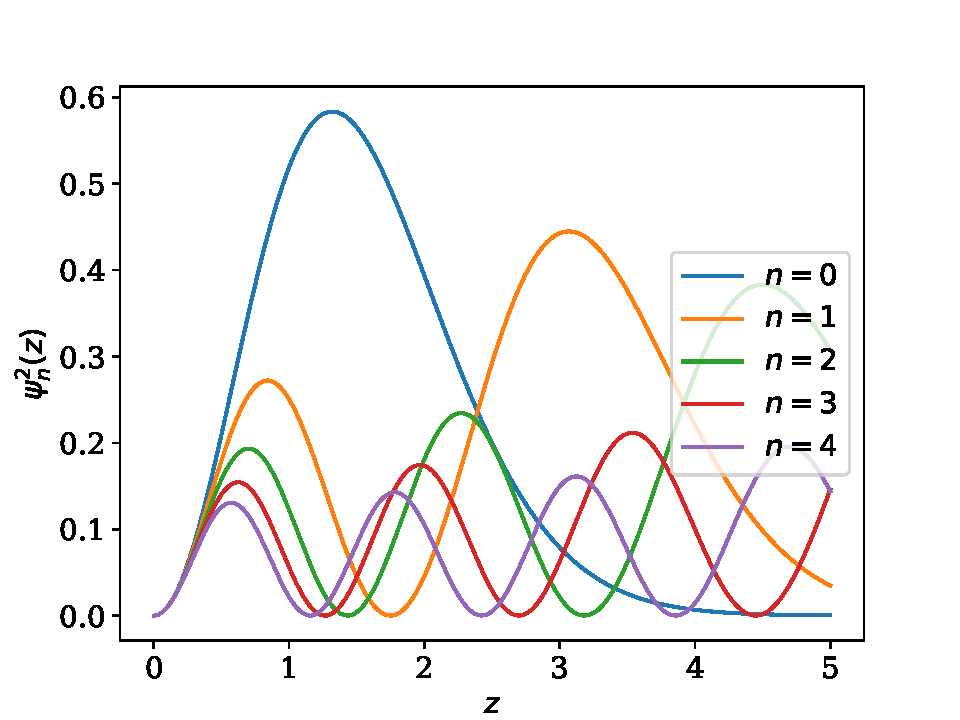
\includegraphics[angle=0,width=15cm ]{finite-size/etats-laser.pdf}
\caption{The scaled probability density function $p(z)$ for the distribution of the height at
a single point for the Airy line given in Eq. (\ref{airyprob})}
\label{1dpot}
\end{center}
\end{figure}
Using this we find the average height is given by
\begin{equation}
\langle h\rangle = \overline h= \ell z_0,
\end{equation}
where 
\begin{equation}
z_0 = \frac{\int_0^\infty dz z {\rm Ai}^2(z-\alpha_1)}{\int_0^\infty dz {\rm Ai}^2(z-\alpha_1)}.
\end{equation}
Interestingly comparison with the thermodynamic calculation giving Eq. \eqref{h1} shows that the identity
\begin{equation}
z_0 = \frac{2}{3}\alpha_1,
\end{equation}
must hold- this surprising identity can be verified numerically. Here we find that the average height given by
\begin{equation}
\langle h\rangle= 0.697089 \ \ell.
\end{equation}
The variance of the magnetisation is then given by
\begin{eqnarray}
\langle M^2\rangle_c &=& -TL\frac{\partial^2}{\partial \lambda^2}f (\lambda)|_{\lambda=0}=-TL\frac{\partial^2}{\partial P^2}f (P)|_{P=P_0}\\
&=& L\frac{\alpha_1 }{2^\frac{1}{3} \sigma^\frac{1}{3}\beta^\frac{5}{3}}\frac{2}{9}P_0^{-\frac{4}{3}}.
\end{eqnarray}
In terms of the average height this then gives
\begin{equation}
\langle M^2\rangle_c = \frac{9}{4\alpha_1^3}L\sigma\beta \overline h^4
\end{equation}


%%%%%%%%%%%%%%%%%%%%
\section{The generalized Lopes-Jacquin-Holdsworth Method}
\label{gen-lopes}
%%%%%%%%%%%%%%%%%%%%
{\color{blue}
In Sec \ref{sec-lopes}, we have shown a way to numerically compute the free energy of a system at a chemical potential $\mu$ in absence of another potential. Here we generalise the method for any kind of external potential. We will explain the method for the Ising model, but the derivation for the SOS model is straightforward.

The Hamiltonian of the SOS model is
\begin{align}
H = - J \sum_{} \sigma_i \sigma_j - \mu \sum_i V(\sigma_i)
\end{align}

where $V(\sigma)$ is a function of the internal microscopic variables $\sigma_i$. The mean value of the external potential is
\begin{align}
    <  \sum_i V(\sigma_i) > =&  \sum_{\bf h} \sum_i V(\sigma_i) \exp(-\beta H) \nn
    =&  - \frac{\partial F(\mu)}{\partial \mu}
\end{align}
where $F$ is the free energy of the system. We see that for any potential of the form \eqref{lopes-gen}, we can integrate the previous equation to find
\begin{align}
   F(\mu_1) - F(\mu_2) = - \int_{\mu_1}^{\mu_2} d\mu'  < \sum_i V(\sigma_i) >_{\mu'} 
   \label{lopes-gen}
\end{align}

In the case where we know the analytical form of the free energy in the limits $\mu_2 \to \infty$ or $\mu_1 \to 0$, this method provides a way to directly measure it for any temperature or size by integrating over the chemical potential.
From the total free energy, we recover the Casimir form through Eq \eqref{cas-lopes}.
The limit $\mu_1 \to 0$ is the free system limit, and the free energy can not be computed analytically.However, when $\mu_2 \to \infty$, for  the majority of external fields $V(\sigma)$ in which we are interested, there is often a configuration limit which whose free energy can be computed analytically. For example, if $V(\sigma)=\sigma$, the configuration limit is the one where all spins point towards the same direction, leading to a free energy of $0$. Thus, we have
\begin{align}
   F(\mu_1) - F_{analytic}(\infty) = - \int_{\mu_1}^{\infty} d\mu'  < \sum_i V(\sigma_i) >_{\mu'} 
   \label{lopes-gen}
\end{align}
In numerical simulations, it is not possible to range over infinity, and a criterion has to be defined to know the error made between the analytic case $\mu_2 = \infty$ and the maximal $\mu_2$ achieved in simulations. As in Eq \eqref{function-d}, we define the function
\begin{align}
    D(\mu,L_1,L_2) =  < M^\ast(L_1)-M^\ast(L_1-1) - (M^\ast(L_2)-M^\ast(L_2-1) >
\end{align}
with the generalized magnetization $M^\ast = \sum_i V(\sigma_i)$. A suitable upper limit of integration if we want to get the Casimir force is when the function $D$ reaches $0$ within the precision of the simulation.


For the SOS Hamiltonian
\begin{align}
    H =  J \sum_i |h_i -h_{i+1}|  + \mu \sum_i V(h_i)
\end{align}
we define the generalised mean height as
\begin{align}
    h^\ast = < \sum_i V(h_i) >
\end{align}
Eqquation \eqref{lopes-gen} writes as
\begin{align}
   F(\mu_1) - F(\mu_2) = -  \int_{\mu_1}^{\mu_2} d\mu' h^\ast(\mu')
   \label{diff-gene}
\end{align}
which can be directly be verified with the transfer matrix. 
In the limit $\mu \to \infty$, the generalised height is zero, while the free energy $F(\infty)$ can often be computed analytically. 
To minimize the error between the analytical limit and the numerical simulations, a suitable choice of the upper integration's limit $\mu_2$ is given by
\begin{align}
    \int_{\mu_2}^\infty  d\mu' h^\ast(\mu')) \ll \int_{\mu_1}^{\mu_2}  d\mu' h^\ast(\mu')
\end{align}
An heuristic argument to find a suitable upper limit for integration is when $h^\ast(\mu_2) \ll h^\ast(\mu_1)$.
In Fig \ref{integration-free-ene}, we see the free energy computed from the matrix transfer, compared to the integration procedure \eqref{lopes-gen} for the SOS model for the chemical potential $V(h_i)=h_i$ in Monte Carlo simulations, where we see the agreement for $\mu_2$ large enough.

\begin{figure}
    \centering
    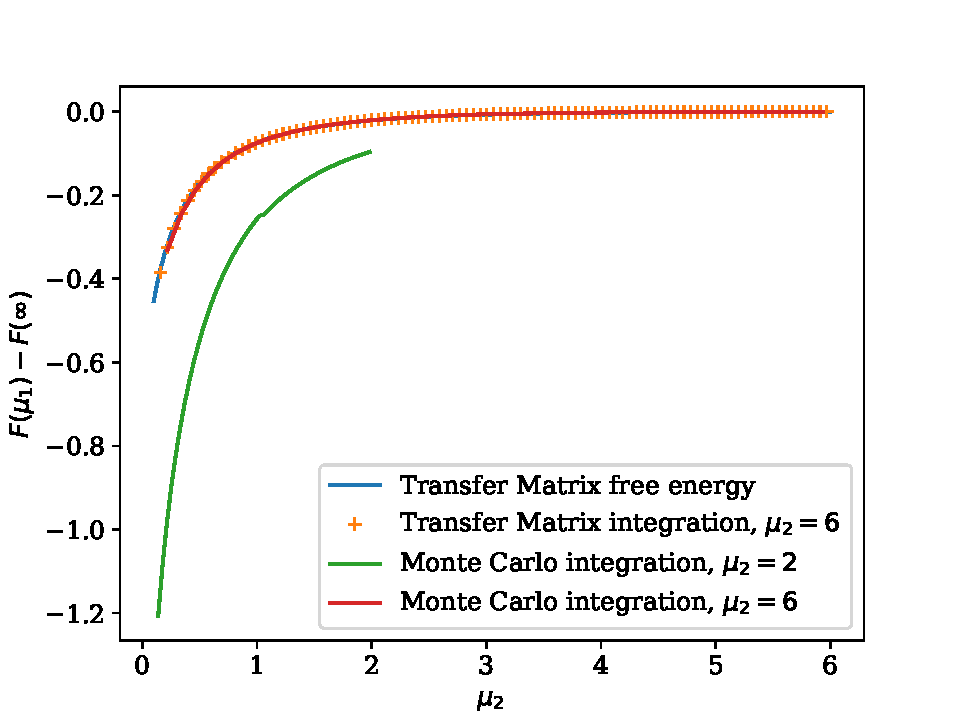
\includegraphics[width=0.7\linewidth]{int-dyn/integration-free-ene.pdf}
    \caption{Difference in free energy directly computed from transfer matrix, compared to numerical integration over the generalized height, for different upper limit $\mu_2$. The parameters are $L' = 256$, $L=200$ and $\beta=1$ for $5e7$ Monte Carlo steps.}
    \label{integration-free-ene}
\end{figure}

Since the order parameter is conserved in model B, the generalized Lopes-Jacquin-Holdswroth method can be used to compute the free energy for Kawasaki dynamics for potentials different from the chemical potential. 
As a proof of concept, we take a potential of the form
\begin{align}
    V(h_i) = - |h_i-\frac{L}{2}|
    \label{neggstaged}
\end{align}
Such potential will press the interface along $h=0$ and $h=L$ compared to the classical chemical potential which presses the interface at $h=0$, as seen in Fig \ref{fig-negstagged}. Far away from $\frac{L}{2}$, both potentials are equivalent in symmetric fashion, and shall behave similarly for large $\mu$, because the free energy only depends on the interface fluctuations and not the mean height. 


\begin{figure}
    \centering
	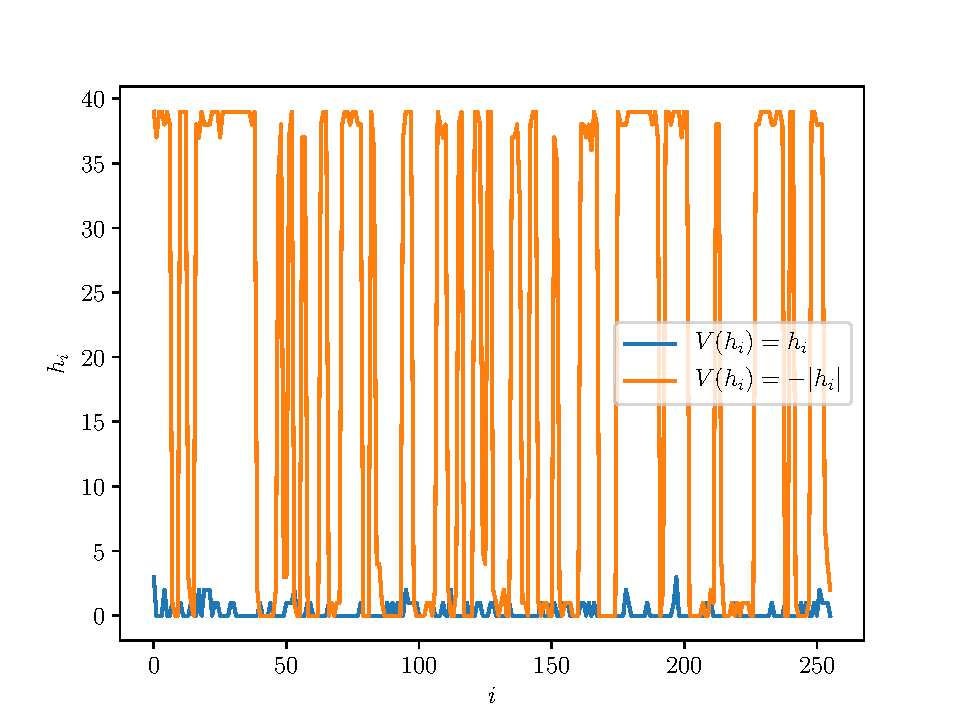
\includegraphics[width=0.7\linewidth]{int-dyn/comp-potentiels-chimiques.pdf}
	\caption{Snapshots of systems for the potential \eqref{neggstaged} and the chemical potential for $\beta=1$ and $\mu=2$ with $L=40$ and $L'=256$}
    \label{fig-negstagged}	
    \centering
   	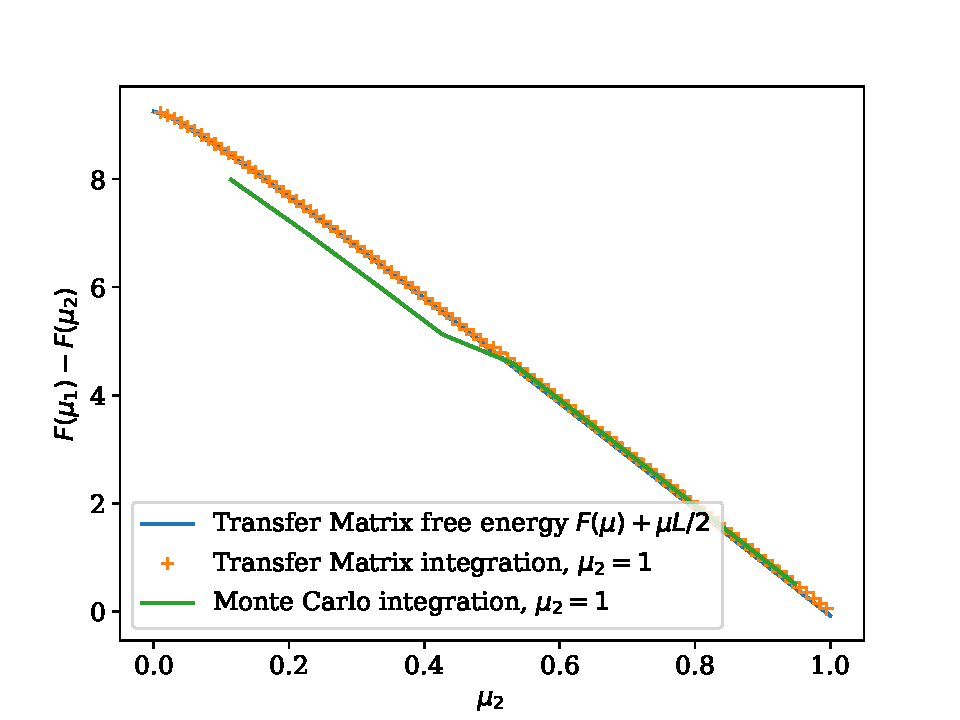
\includegraphics[width=0.7\linewidth]{int-dyn/integration-free-ene-negstagged.pdf}
    \caption{Difference in free energy directly computed from transfer matrix with the potential \eqref{neggstaged}, compared to numerical integration over the generalized height. The parameters are $L' = 256$, $L=20$ and $\beta=1$, $\mu_2 = 1$for $10^7$ Monte Carlo steps. } 
   	\label{fig-int-negstagged}    
\end{figure}  

In the $\mu \rightarrow \infty$ limit, the system has two equilibrium positions $h=0$ et $h=L$, which gives the transfer matrix
\begin{align}
T= e^{\beta \mu \frac{L}{2}}
  \begin{pmatrix}
    1 & e^{-\beta  J L} \\
    e^{-\beta  J L} & 1
  \end{pmatrix}
\end{align}
The eigenvalues are $\lambda_\pm = e^{ \beta \mu \frac{L}{2}}( 1 \pm e^{-\beta J L})$, which gives us the free energy 
\begin{align}
  F(\mu \rightarrow \infty) = - \mu \frac{L}{2}
\end{align}
We plotted in Fig \ref{fig-int-negstagged} the difference of free energy computed from the transfer matrix between $\mu_1$ finite and $\mu_2=1$, and the integration procedure \eqref{diff-gene} with the generalized height with the matrix transfer and Monte Carlo simulations, both for Glauber and Kawasaki dynamics. The disagreement between the expected value and the simulation results are from a $\mu_2$ too small, which we also see in the integration of the generalized height from the transfer matrix. We can convince ourselves by doing the integration from the transfer matrix for a larger $\mu_2$. Also, it is worth noting that for this system, there is no significant difference between both dynamics.

This method opens a new way to compute the free energy for any kind of external potential of the form $\mu V(h)$, or $\mu V(\sigma)$ in the case of the Ising or SOS models for conserved and non-conserved dynamics, such as non-uniform external fields \cite{bissacot_phase_2010}. 
}


%%%%%%%%%%%%%%%%%%%%
\section{The confined solid on solid model}
%%%%%%%%%%%%%%%%%%%%

{\color{blue}
From exact diagonalization of the SOS transfer matrix in the infinite case \cite{guyer_sine-gordon_1979}, finite-size effects were studied both for the SOS and RSOS model \cite{svrakic_finite-size_1988,privman_finite-size_1988}. Nevertheless the derivation of eigenvectors and eigenvalues were not explicit in the latter case. Those eigenvalues are a multiple of an integer, and the study of the eigenvalues issued from an odd integer where also not discussed. We also add an analysis to the correlation length and the limits of high and low temperatures for the free energy. 

We consider here the free interface confined between $0$ and $L$, with no external field.} {\color{red} The SOS transfer matrix is thus given by 
\begin{align}
T(h_i,h_j) = \exp(-\beta J |h_i-h_j|)
\end{align}
Since positions are comprised from $0$ to $L$, we can write the transfer matrix as}
\begin{equation}
T_{ij} = \exp(-\beta J|i-j|).
\end{equation}
We introduce 
\begin{equation}
r=\exp(-\beta\ J)
\end{equation}
To find the eigenvectors of $T$, we consider the vector denoted by $[a]$ which has components
\begin{equation}
[a]_i = a^i,
\end{equation}
where $i$ is an index ranging from $0$ to $L$. 
The action of the SOS transfer matrix on this vector is given by
\begin{equation}
\left[T\ [a]\right]_i = \sum_{j=0}^L r^{ |i-j|} a^j
\end{equation}
and we find
\begin{align}
[T\ [a]]_i
=& r^i \sum_{j=0}^i r^{-j} a^j + r^{-i} \sum_{j= i+1}^L r^j a^j \nn
=& r^i \sum_{j=0}^i r^{-j} a^j + r^{-i} \sum_{k= 0}^{L-i-1} r^{i+1+k} a^{i+1+k} \nn
=& r^i \frac{1- r^{-(i+1)} a^{i+1}}{1- r^{-1} )a} + r a^{i+1}\frac{1- r^{L-i} a^{L-i}}{1- r a} \nn
=&\left[\frac{ ra}{1-ra}- \frac{ \frac{a}{r}}{1-\frac{a}{r}}\right]a^i +\frac{r^i}{1-\frac{a}{r}}-\frac{r^{L+1-i}a^{L+1}}{1-ra}
\end{align}
We now define
\begin{equation}
\lambda(a)= \frac{ ra}{1-ra}- \frac{ \frac{a}{r}}{1-\frac{a}{r}} = \frac{\frac{1}{r}-r}{\frac{1}{r}+r
- a-\frac{1}{a}}
\label{elam}
\end{equation}
and notice that
\begin{equation}
\lambda(a) = \lambda(a^{-1})
\end{equation}
We can thus write
\begin{equation}
[T\ [a]]_i= \lambda(a)a^i +\frac{r^i}{1-\frac{a}{r}}-\frac{r^{L+1-i}a^{L+1}}{1-ra}
\end{equation}
Now, considering the action of the transfer matrix on the vector $[a^{-1}]$, we find
\begin{equation}
\left[T\ [a^{-1}]\right]_i = \lambda(a) a^{-i} + \frac{r^i}{1-\frac{1}{ra}}-\frac{r^{L+1-i}a^{-(L+1)}}{1-\frac{r}{a}}
\end{equation}
We now look for an eigenvector of the form
\begin{equation}
{\bf v} = [a]+ c[a^{-1}]
\end{equation}
The action of $T$ on ${\bf v}$ is 
\begin{equation}
\left[T\ ([a]+c [a^{-1}]\right]_i = \lambda(a)[a^i + c a^{-i}]
+ r^i\left(\frac{1}{1-\frac{a}{r}}+ \frac{c}{1-\frac{1}{ra}}\right)
- r^{L+1-i} \left(\frac{a^{L+1}}{1-ra} + c\frac{a^{-(L+1)}}{1-\frac{r}{a}}\right)
\end{equation}
and we see that ${\bf v}$ is an eigenvector, with eigenvalue $\lambda(a)$, if
\begin{eqnarray}
\frac{1}{1-\frac{a}{r}}+ \frac{c}{1-\frac{1}{ra}}&=&0 \\
\frac{a^{L+1}}{1-ra} + c\frac{a^{-(L+1)}}{1-\frac{r}{a}} &=& 0
\end{eqnarray}
The above equations imply that 
\begin{equation}
c= -\frac{ra-1}{a(r-a)}
\end{equation}
and
\begin{equation}
c^2 = a^{2L}
\end{equation}
Therefore we find
\begin{equation}
v_i = a^i \pm a^{L-i}
\end{equation}

\subsubsection*{Ground state eigenvector}
We expect the ground state eigenvector (corresponding to the largest eigenvalue) to be symmetric with respect to the middle of the system and so 
\begin{equation}
v_i= v_{L-i}
\end{equation}
which implied that we should have $c= a^L$. 

This then gives the equation determining the values of a for the largest eigenvalue, and in general for the eigenvalues which are symmetric ( $c=1$),
\begin{equation}
a^{L+1} = \frac{1-ra}{r-a}.
\label{aeq}
\end{equation}

As a check on the above derivation we can consider the case $L=1$ so we have two sites. Here we see that the transfer matrix is given explicitly by
\begin{equation}
T =\begin{pmatrix} & 1 & r\\& r &1\end{pmatrix}
\end{equation}
and the largest eigenvector is easily seen to be given by
\begin{equation}
\lambda_0 = 1+r 
\end{equation}
In this case, we seethat Eq. (\ref{aeq}) gives
\begin{equation}
a^{2} = \frac{1-ra}{r-a}
\end{equation}
which has three solutions
\begin{eqnarray}
a_1&=& -1\\
a_2&=& \frac{1}{2} \left(-\sqrt{r^2+2
r-3}+r+1\right) \\
a_3&=& \frac{1}{2} \left(\sqrt{r^2+2
r-3}+r+1\right)\end{eqnarray}
We see that $a_2=1/a_3$, and $|a_2|=|a_3|=1$, and that
\begin{equation}
\lambda(-1)= \frac{1-r}{1+r}
\end{equation}
while 
\begin{equation}
\lambda(a_2)=\lambda(a_3)= 1+r
\end{equation}
corresponds to the maximal eigenvalue. Note that $\lambda(-1)$ is not the other eigenvalue of the transfer matrix, this has to be found by considering solutions with $c=-1$, as we will see later.

The equation (\ref{aeq}) determining $a$ can also be written as
\begin{equation}
a^{L} = - \frac{r-\frac{1}{a}}{r-a}
\end{equation}
From this we see that if $a$ is a solution then $1/a$, and that $a=-1$ is always a solution.


We now introduce $\theta$ and 
\begin{align}
a=\exp(i\theta)
\label{def-theta}
\end{align}
Then the parameter of the eigenvector is
\begin{equation}
\exp(i L \theta) = - \frac{r-\exp(-i\theta)}{r-\exp(i\theta)}
\label{thetamas}
\end{equation}
From Eq \eqref{elam}, we have
\begin{equation}
\lambda(\theta) = \frac{\sinh(\beta J)}{\cosh(\beta J) - \cos(\theta)}.
\end{equation}
Notice that in order to construct a real eigenvector corresponding to $\lambda_0$ we can use the fact that both $v_i(a) = a^i + a^{L-i}$ and $v_i(a^{-1}) = a^{-i} + a^{-L+i}$ are both eigenvectors with the same eigenvalue. This means that $u_i(a) = v_i(a) + v_i(-a)$ is also an eigenvector and all its components are real. 

Clearly the largest eigenvalue corresponds to the value of $\theta$ closest to $0$,  so we look for an eigenvalue such that $L \theta \sim 1$. We write
\begin{equation}
\phi = L \theta
\end{equation}
For $L$ large, this gives
\begin{equation}
\exp(i\phi) \approx -\frac{r-1+ i\frac{\phi}{L}}{ r-1- i\frac{\phi}{L}}\approx -1 +2 i\frac{\phi}{L(1-r)}
\end{equation}
and so we find to leading order in $1/L$
\begin{equation}
\theta = \frac{(2n+1)\pi}{L}
\end{equation}
However we notice that this approximation is only valid if $L(1-r) \gg1$. For large $\beta$ this approximation is simply equivalent to $L\gg1$, however when $\beta$ is small it requires
that $H \beta \gg 1$.

The closest eigenvector to the real axis has $n=0$ and so we have
\begin{equation}
\lambda_0 \approx \frac{\sinh(\beta J)}{\cosh(\beta J) - \cos(\frac{\pi}{L})} \approx \frac{\sinh(\beta J)}{\cosh(\beta J) - 1+ \frac{\pi^2}{2 L^2}} \approx \coth(\frac{\beta J}{2})(1 - \frac{\pi^2}{4\sinh^2(\frac{\beta J}{2}) L^2})
\label{ground-sos}
\end{equation}
{\color{red} In the limit $L\to \infty$, the ground-state eigenvalue is the same as the Sine-Gordon chain of length $L' \to \infty$ fixed at $h(0) = h(L') = 0$ and using a SOS interaction between nearest neighboors \cite{guyer_sine-gordon_1979}, which is normal since boundary conditions on the x-axis are negligible in the thermodynamic limit.}

\subsubsection*{First excited state eigenvector}
In order to compute the second eigenvalue $\lambda_1$ we look for an odd or antisymmetric solution with $c=-1$. We thus find
\begin{equation}
\exp(i L\theta) = \frac{r-\exp(-i\theta)}{r-\exp(i\theta)}
\label{theta}
\end{equation}

For large $L$ we look for a solution of the form $\theta=\phi/L$ and this gives
\begin{equation}
\exp(i\phi) \approx 1
\end{equation}
and so we chose solutions $\phi = 2n\pi$ for integer $n$. However the solution $n=0$ which corresponds to $a=1$ has $v(i) = a^i-a^{L-i} =0$ and so does not correspond to an eigenvector. We thus take the next solution $\phi = 2\pi$ which gives
\begin{equation}
\lambda_1 \approx \frac{\sinh(\beta J)}{\cosh(\beta J) - \cos(\frac{2\pi}{L})} \approx \frac{\sinh(\beta J)}{\cosh(\beta J) - 1+ \frac{2\pi^2}{L^2}}\approx \coth(\frac{\beta J}{2})(1 - \frac{\pi^2}{\sinh^2(\frac{\beta J}{2}) L^2})
\label{excited-sos}
\end{equation}
In Fig \ref{large-l-limit}, we show the agreement between the computation of the first two eigenvalues !!!! computed by numerical diagonalisation and compared with the analytical approximations Eq. \eqref{ground-sos} and Eq. \eqref{excited-sos} which are valid for the large L limit
\begin{figure}
\centering
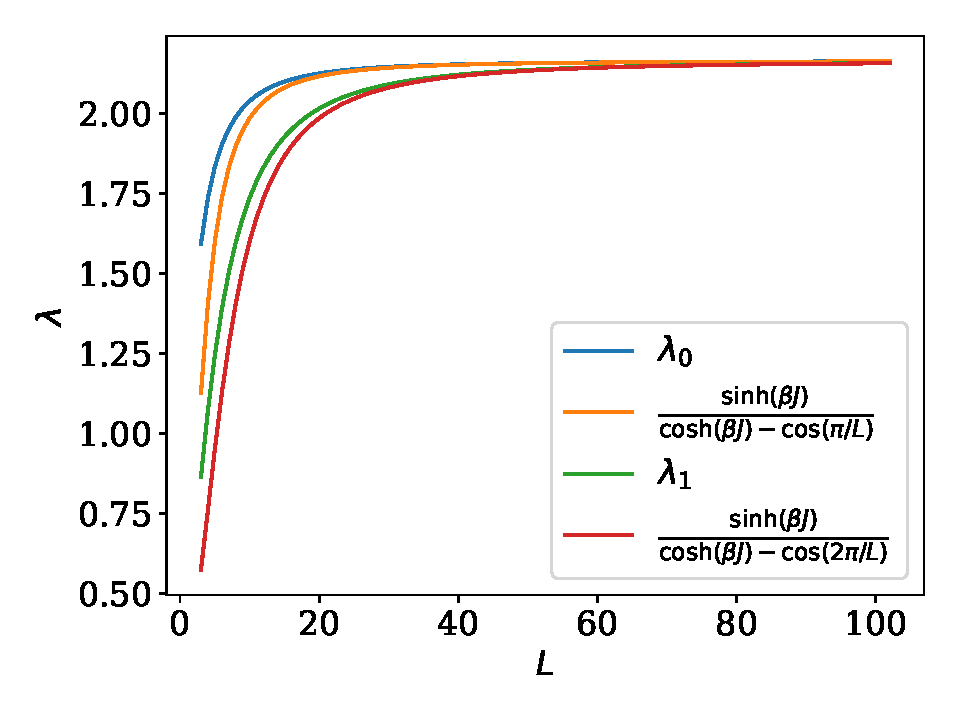
\includegraphics[width=0.7\linewidth]{finite-size/null_deanJ.pdf}
\caption{$\lambda_0$ and $\lambda_1$ as a function of $L$ computed by numerical diagonalisation of the transfer matrix, compared to the analytical approximations for large $L$: Eq. \eqref{ground-sos} and Eq. \eqref{excited-sos}. Here we have chosen  for $J=1$ and $\beta=1$.}
\label{large-l-limit} 
\end{figure}

The correlation length is then given by
\begin{equation}
\xi =\frac{1}{\ln(\frac{\lambda_0}{\lambda_1})} = \frac{1}{\ln(\frac{\cosh(\beta J) - \cos(\frac{\pi}{L})}{\cosh(\beta J) - \cos(\frac{2\pi}{L})})}\approx \frac{4}{3}\frac{\sinh^2(\frac{\beta J}{2})L^2}{\pi^2}
\end{equation}
and we see that this has the same form as that for the free elastic line in Eq. (\ref{corel}).
Furthermore, the free energy per site is given in the thermodynamic limit and for large $L$ by
\begin{equation}
f=-\frac{1}{\beta}\ln(\lambda_0) \approx -\frac{1}{\beta}\left[ \ln(\coth(\frac{\beta J}{2}))- \frac{\pi^2}{4\sinh^2(\frac{\beta J}{2}) L^2}\right]
\end{equation}
and this gives a pressure
\begin{equation}
P= -\frac{\partial f}{\partial L}= \frac{T\pi^2}{2 J\sinh^2(\frac{\beta}{2}) L^2}.
\end{equation}
This has the same form as the pressure for the elastic line in Eq. (\ref{pfree}) if we make the identification of the effective surface tension to be used in the elastic line model
\begin{equation}
\sigma_{eff} = \frac{2}{\beta}\sinh^2(\frac{\beta J}{2})
\end{equation}
We should note that this is also consistent with the equality deduced by comparing the correlation length of the two models.

We see that in the limit of large $L$ and for appropriately low temperatures, the finite size SOS model reproduced the phenomenology of the elastic line (confined Edwards-Wilkinson surface). 
This is not surprising as a low temperatures jumps of more that two lattice spacings in the height are suppressed by a factor or $\exp(-\beta J)$ with respect to staying at the same height moving up or down by one site. The low temperature SOS model thus becomes effectively equivalent to the RSOS model and thus is equivalent to a local random walk model. 

\subsubsection*{High temperature limit}

To explore the high temperature limit we can note that if we write
\begin{equation}
z= r-\exp(-i\theta)
\end{equation}
we can write Eq. \eqref{thetamas} as
\begin{equation}
\exp(i L\theta) = -\frac{z}{\overline z} = \exp(2i\psi + i\pi)
\end{equation}
where
\begin{equation}
\tan(\psi) = \frac{\sin(\theta)}{r-\cos(\theta)}
\end{equation}
This then gives 
\begin{equation}
L \theta = 2\psi + \pi
\end{equation}
and so
\begin{equation}
\tan(\psi) = \frac{\sin(\theta)}{r-\cos(\theta)}= \tan(\frac{L\theta}{2} +\frac{\pi}{2})= - \cot(\frac{L\theta}{2})
\end{equation}
which finally gives
\begin{equation}
\tan(\frac{L\theta}{2}) = \frac{\cos(\theta)-r}{\sin(\theta)}
\label{mde}
\end{equation}
In this form we see that our calculations agree with those of Svravick et al \cite{svrakic_finite-size_1988}. Futhermore when $\beta\to 0$ we know that the elements of the transfer matrix all tend to one and that the largest eigenvalue has all components equal. This means that in the infinite temperature limit, $\theta=0$. Therefore in Eq. \eqref{mde} we look for solutions where $\theta$ is small. Taylor expanding gives to leading order
\begin{equation}
\frac{L\theta^2}{2} \approx1-r-\frac{\theta^2}{2}
\end{equation}
which gives
\begin{equation}
\theta \approx \sqrt{\frac{2(1-r)}{L+1}}
\end{equation}
However the above expansion assumes that $\theta L\ll1$ and so
\begin{equation}
\sqrt{2L(1-r)} \ll 1
\end{equation}
This means that the height can fluctuate by of order $L$ from site to site. The high temperature approximation is thus equivalent to
\begin{equation}
\theta \approx \sqrt{\frac{2\beta J}{L+1}}.
\end{equation}
Therefore at high temperature this means that $L \beta J\ll1$. 
This gives a maximal eigenvalue
\begin{equation}
\lambda_0 = L+1
\end{equation}
and the free energy
\begin{equation}
f=-\frac{1}{\beta}\ln(L+1)
\end{equation}
which is the obvious result coming from the infinite temperature entropy. 
This result suggests that the solution for $\theta$ at small $\beta$ can be written as a perturbation series of the form
\begin{equation}
\theta = \sqrt{\beta J}\sum_{n=0}^\infty b_n (\beta J)^n
\end{equation}
The first two terms give
\begin{equation}
\theta = \sqrt{\beta J}\left[\sqrt{\frac{2\beta J}{L+1}} -\beta J \frac{2 + 2L +L^2}{6\sqrt{2}(1+L)^{\frac{3}{2}}}\right]
\end{equation}
and from this we find
\begin{equation}
f=-\frac{1}{\beta}\ln(L+1-\beta J\frac{L^2+2L}{3})
\label{high-temperature} 
\end{equation}
{\color{red} and where we show in Fig \ref{fig-high-temp} the agreement of the high-temperature approximation \eqref{high-temperature} with respect to the direct diagonalization of the transfer matrix.}
As pointed out above this result gives the high temperature entropy but it also exhibits the correct average energy $\epsilon$ per unit length at high temperature. To see this we note that all values of $h$ are equiprobable at infinite temperature and so
\begin{equation}
\epsilon = \frac{1}{(L+1)^2} J \sum_{i,j=0}^L |i-j| = J\frac{L^2+2L}{3}
\end{equation}

\begin{figure}
\centering
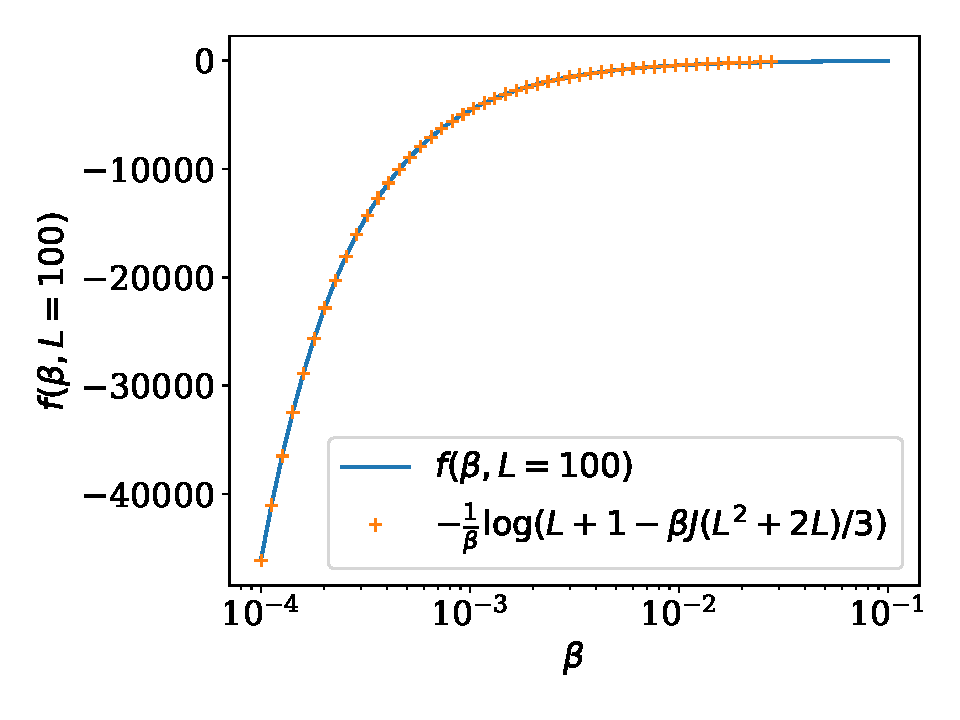
\includegraphics[width=0.7\linewidth]{finite-size/high_temperature.pdf}
\caption{Free energy with respect to $\beta$ for $L=100$ and $J=1$ in the high-temperature limit, by direct diagonalization of the transfer matrix and by Eq \eqref{high-temperature}.}
\label{fig-high-temp} 
\end{figure}


%%%%%%%%%%%%%%%%
\section{Conclusion}
%%%%%%%%%%%%%%%%
{\color{red}
Finite-size effects occur in all kind of statistical systems. In this chapter, we have made a brief review of the confinement forces, first for the electromagnetic field in vacuum \cite{h_b_g_casimir_attraction_1948,boyer_quantum_1968,milton_casimir_1978,bowers_casimir_1998,sm_rytov_principles_1989,lifshits_theory_1955}
for critical systems \cite{gambassi_casimir_2009} . When the correlation length of the field becomes of the same order of magnitude as the size of the system confinement forces arise because of the suppression of the soft modes. 
Using the propagator method \cite{matsubara_new_1955} , we have then shown that for continuous free interfaces the confinement force is Casimir-like. When adding a chemical potential, we have computed the average height of the interface, the ground-state energy and the confinement force, which is also Casimir-like.
We have also generalized the Lopes-Jacquin-Holdsworth method \cite{lopes_cardozo_critical_2014} , which is useful to measure the free energy of a system through integration of the field conjugated to the integration parameter. This allows us to compute the free energy both in Glauber and Kawasaki dynamics, and have shown an agreement between both statistical ensembles.
In the last section, we extended some results over the SOS transfer matrix \cite{guyer_sine-gordon_1979,privman_finite-size_1988}, computing the eigenvalues in the large size limit or the high-temperature limit.}
\chapter{Beyond Solid-On-Solid : the Particles-Over-Particles model}

In fact, if the height profiles represent particle numbers, if we fix the total number of particles to be $N$ and take them to be identical the partition function is given by
\begin{equation}
    Z_N = \frac{1}{N!}\sum_{h_1,h_2\cdots h_L} \delta_{\sum_{i=1}^L h_i, N}\frac{N!}{\prod_{i=1}^L h_i!} \exp\left(-\beta \sigma \sum_{i=1}^L |h_{i+1}-h_i| -\beta\sum_{i=1}^L V(h_i)\right).
\end{equation}
Here the combinatorial term $\frac{N!}{\prod_{i=1}^L h_i!}$ represents the number of ways that the $h_i$ particles on each site can be chosen from the $N$ particles available. The constraint on the particle number makes the computation of the partition function at fixed $N$ complicated both analytically and numerically. However if we change to the grand canonical ensemble using
the formula
\begin{equation}
    \Theta = \sum_{N} \exp(\beta\mu N) Z_N,
\end{equation}
where $\Theta$ is the grand partition function and $\mu$ the chemical potential, we find
\begin{equation}
    \Theta = \sum_{h_1,h_2\cdots h_L} \frac{1}{\prod_{i=1}^L h_i!} \exp\left(-\beta \sigma \sum_{i=1}^L |h_{i+1}-h_i| -\beta\sum_{i=1}^L[ V(h_i)-\mu h_i]\right).
\end{equation}
The grand partition function can then be written as 
\begin{equation}
    \Theta = \sum_{h_1,h_2\cdots h_L} \exp\left(-\beta H_{eff}(h_1,h_2\cdots h_L)\right)
\end{equation}
where 
\begin{equation}
    H_{eff}= \sigma \sum_{i=1}^L |h_{i+1}-h_i| +\sum_{i=1}^L [V(h_i)-\mu h_i +\frac{1}{\beta}\ln(h_i !)].
\end{equation}

\begin{figure}
    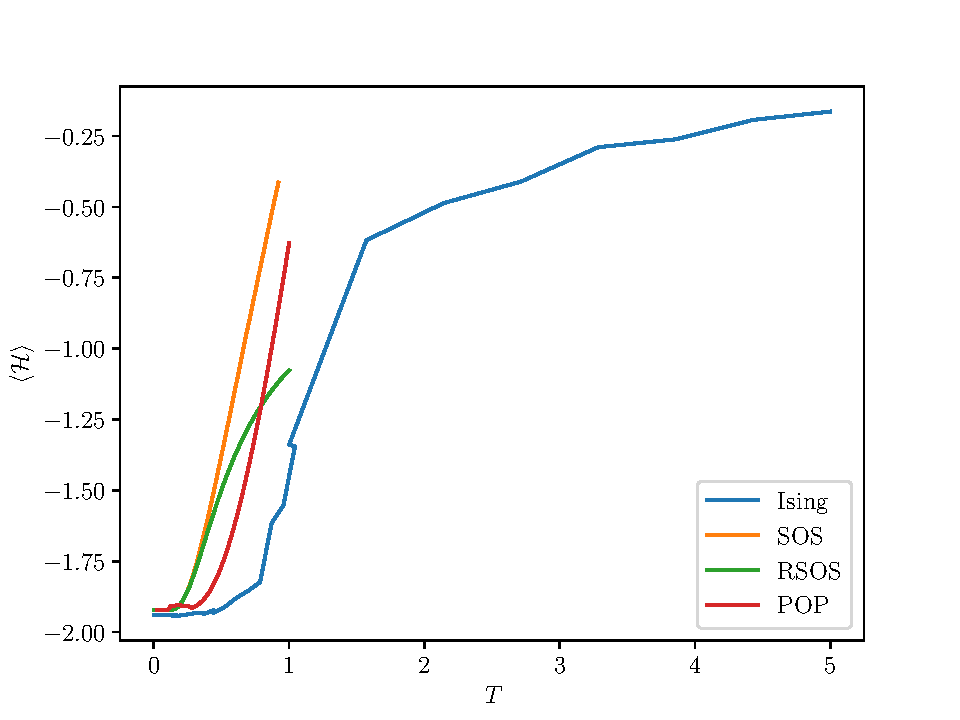
\includegraphics{pop/comparaison-modeles.pdf}
\end{figure}
\begin{figure}
    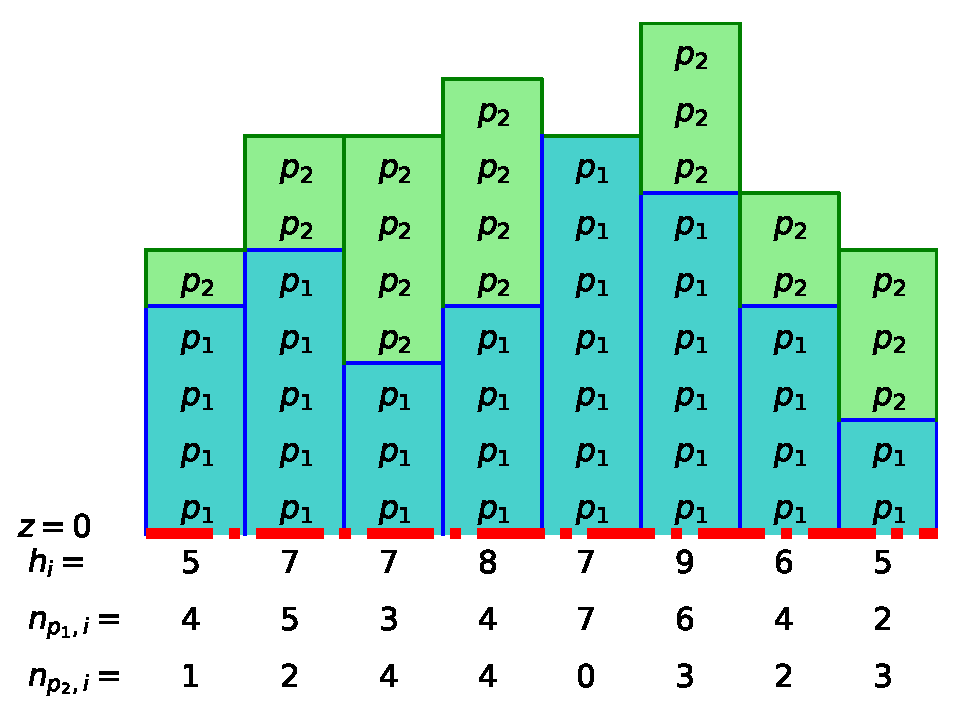
\includegraphics{pop/figure-pop.pdf}
\end{figure}
%%%%%%%%%%%%%%%%
\chapter{Driven model C interfaces}
%%%%%%%%%%%%%%%%
We consider the effect of uniform driving on the interface between two phases which are described by model C dynamics. The non-driven system has a classical Gaussian interface described by capillary wave theory. The model under driving retains Gaussian statistics but the interface statistics are modified by driving, notably the height fluctuations are suppressed and  the correlation length of the fluctuations is increased.

%%%%%%%%%%%%%%%%
    \section{Introduction}
%%%%%%%%%%%%%%%%

The model we introduce can also be used as a model for the effect of activity on interface dynamics.
One of the most natural ways of creating a non-equilibrium steady state is by applying external  driving forces. Driving arises naturally in sedimenting systems due to gravity, in systems with free charges under the action of an electric field and also  due to the radiation pressure exerted by a laser. Experiments where a phase separated colloidal system is sheared parallel to the interface show that  driving due to shear tends to suppress surface fluctuations \cite{derks2006},
and similar results are found where Ising models are numerically sheared 
\cite{smith2008,smith2010}. These results are somewhat surprising, for instance they are contrary to the  observation that wind generates waves on the ocean. One may think that the precise nature of the driving plays a role, for instance uniformly driving a system may be intrinsically different to applying a shear field which is manifestly nonuniform. In this paper we investigate analytically the effect of uniform driving on a simple interface model. We find that the effect of this type of  driving is also to reduce surface fluctuations.

Constructing a continuum model which is analytically tractable and is also 
affected by uniform driving is straightforward but contains some subtleties. 
In a continuum system it is clear that uniform driving can only move a system away from equilibrium when the driving acts differently on different particle types. For instance, consider  a system of identical interacting Brownian particles driven by a uniform  force. The force will induce the same average velocity on all the particles, consequently, in the frame moving with this average velocity, we will recover the unmodified equilibrium state. However, when multiple particle types are present, the mean velocity induced on different species are different and no Galilean transformation is possible. Perhaps the first such study of this phenomenon was due to Onsager \cite{hem1996}, who studied the conductivity of electrolytes and in doing so showed how the correlation functions in the steady state were modified by the electric field. 
Recently there have been many studies of driven multi-particle Brownian systems \cite{netz2003,dzub2002,chak2003,chak2004,lowe2009,glan2012, klym2016}, including the electrolyte problem,  and rich new physics has been found, even in the case of purely Gaussian theories \cite{dem2016,pon2017} based on stochastic density functional theory \cite{dean1996}. 

The dynamics of discrete particle systems is however affected by uniform driving of identical particles. The study of driven lattice gases has revealed a wide range of intriguing physical phenomena and indeed shown how driving can even lead to phase separation \cite{katz1984,zia1991,leun1993,schm1995,schm1998}. The discrete nature of the dynamics of these systems, both in space and time, means that no Galilean transformation to an equilibrium state exists. Analytical studies of these systems require a phase ordering kinetics description in terms of a continuum order parameter. In order to break Galilean invariance the local mobility of the particles can be taken to be dependent on the local order parameter, this is then sufficient to induce non-trivial steady states under driving \cite{katz1984,leun1993,schm1995,schm1998}. Interfaces between the separated phases in uniformly driven systems have non capillary behaviors which are, even today, not fully understood \cite{leun1993}.
Taking random driving in a given direction also leads to non-equilibrium steady states, if the noise is Gaussian and white, the fluctuation dissipation theorem is violated and novel interface fluctuations are induced which, again, are  not of  the capillary type \cite{zia1991}. 

Driving can also be deterministic but space dependent, for instance if one considers applied shear flows, the spatial dependence of the flow means no Galilean transformation to an equilibrium steady state is possible and this therefore leads to non-equilibrium steady states. The effect of shear on interfaces in these type of systems yields interface equations of the stochastic Burgers type and the statistics are no thus longer Gaussian due to the presence of nonlinearities \cite{bray2001,bray2002,smith2008,smith2010,thie2010,thie2014}. 

In this paper we analyse what is known, in the classification of Hohenberg and Halperin \cite{hohe1977}, as model C type dynamics for two fields, one with conserved model B type dynamics, which is in addition convected at a uniform velocity to mimic driving. We refer to this first field as the colloid field.
This colloid field is coupled to an additional field which undergoes model A non-conserved dynamics and which is not subjected to the driving. The model A field can be thought of a passive solvent and its coupling to the model B field is chosen in such a way that it has no influence on the non-driven equilibrium steady state. We then derive the effective dynamics between two separated low temperature phases by using a
method introduced in \cite{bray2001,bray2002} for the study of interfaces under shear flow. This method yields a Gaussian theory for the interface statistics and driving introduces interesting new physics, notably we find that the effective surface tension of the system is increased but also the correlation length of interface fluctuations (due to an effective gravitational term) are increased. These observations are in qualitative agreement with experimental results on sheared low tension interfaces in phase separated colloidal systems \cite{derks2006}. In this experimental system the interface fluctuations were also found to be well described by Gaussian statistics and this is our principal motivation for studying theories which remain Gaussian but are  modified by driving. While the long wavelength theory we find is of a capillary type, we also find new, higher derivative terms, which  are generated in the spectrum of the height fluctuations. 

As an aside, we also show how the model introduced here can be used to analyse the effect of activity on the dynamics of the surface between two phases of active colloids. The activity is implemented by taking a different temperature for the colloid and solvent fields, this difference in temperatures leads to significantly modified surface statistics which again develop dependencies on static and dynamical variables of the model which otherwise remain hidden for the equilibrium version of the problem.

%%%%%%%%%%%%%%%%
    \section{The underling two field  model}
%%%%%%%%%%%%%%%%

We consider a coarse grained model for two scalar fields $\psi$ and $\phi$ with Hamiltonian
\begin{equation}
    H[\psi,\phi] = H_1[\psi] +H_2[\psi,\phi]
\end{equation}
The Hamiltonian $H_1$ is of the classic Landau-Ginzburg form
\begin{equation}
    H_1[\psi]=\int d\bx\left[\frac{\kappa}{2}[\nabla\psi(\bx)]^2 + V(\psi(\bx))
- gz \psi(\bx)\right].
\end{equation}
The last term represents the energy due to a gravitational field and will introduce a finite correlation length in the fluctuations between the two phases. We assume that the above Hamiltonian has two stable phases with average concentrations of the field $\phi(\bx)$ given by the constant values $\psi_1$ and $\psi_2$, the difference between the order parameter in  the two different phases is denoted by 
by $\Delta\psi= \psi_2 -\psi_1>0$. This means that we find the phase $1$ as $z\to\infty$ and the phase $2$ as $z\to-\infty$. The term $H_2$ is taken to be a simple quadratic coupling between the fields
\begin{equation}
    H_2 =\int d\bx \frac{\lambda}{2}(1-\psi(\bx)-\phi(\bx))^2,
\end{equation}
this is an approximative conservation law of total volume fraction of the phases. The field $\phi$ can be though of as the local volume fraction of the solvent in a colloidal system. However the presence of this solvent field does not change the effective equilibrium statistical mechanics of the colloid field $\psi$ as the partition function can be written as 
\begin{equation}
    Z = \int d[\phi]d[\psi]\exp(-\beta H_1[\psi]- \beta H_2[\psi,\phi]) = CZ_{eff},
\end{equation}
where $Z_{eff}$ is the effective partition function for the field $\psi$, after we have integrated out the degrees of freedom corresponding to the field $\phi$,
and $C$ is a constant term resulting from this integration. The effective partition function is thus simply given by
\begin{equation}
    Z_{eff} = \int d[\psi]\exp(-\beta H_1[\psi]),
\end{equation}
and, as stated above, we see that the field $\phi$ thus has no effect on the equilibrium statistical mechanics of the field $\psi$.

We now consider the dynamics of the fields. We take local diffusive model B dynamics for the field $\psi$ and non-conserved model A dynamics for the field $\phi$
\begin{eqnarray}
\frac{\partial \psi(\bx,t)}{\partial t} +{\bf v}\cdot { \nabla}\psi(\bx,t)&=& D\nabla^2\frac{\delta H}{\delta \psi(\bx)}+ \sqrt{2D T}\nabla \cdot {\bm \eta}_1(\bx,t) \\
\frac{\partial \phi(\bx,t)}{\partial t} &=& -\alpha\frac{\delta H}{\delta \phi(\bx)}+ \sqrt{2\alpha T}{ \eta}_2(\bx,t).
\end{eqnarray}
The first equation corresponds to standard model B dynamics but with an advection term by a constant velocity field $\bf v$. The second equation has no advection term and is simple model A dynamics. In principle we can also treat the case where the dynamics of the field $\phi$ is also diffusive and thus of model $B$ type, the analysis given here can be extended to this case but the analysis of the resulting equations is considerably more complicated. The use of model A dynamics for the solvent is justified by assuming that its dynamics is faster than that of the colloids and that the volume fraction can vary due to local conformational changes rather than  diffusive transport.

The noise terms above 
are uncorrelated and Gaussian with zero mean, their correlation functions are given by
\begin{eqnarray}
< \eta_{1i}(\bx,t) \eta_{1j}(\bx',t)>&=& \delta_{ij}\delta(t-t') \delta(\bx-\bx') \\
< \eta_{2}(\bx,t) \eta_{2}(\bx',t)>&=& \delta(t-t') \delta(\bx-\bx') ,
\end{eqnarray}
and $T$ is the temperature in units where $k_B=1$.
These dynamical equations  are thus explicitly given by
\begin{equation}
    \frac{\partial \psi(\bx,t)}{\partial t} +{\bf v}\cdot { \nabla}\psi(\bx,t)= D\nabla^2[\frac{\delta H_1}{\delta \psi(\bx)}+\lambda(\phi(\bx,t) + \psi(\bx,t))]+ \sqrt{2D T}\nabla \cdot {\boldsymbol \eta}_1(\bx,t)
\end{equation}
and
\begin{equation}
    \frac{\partial \phi(\bx,t)}{\partial t} = -\alpha\lambda[\phi(\bx,t) + \psi(\bx,t)]+ \sqrt{2\alpha T}{ \eta}_2(\bx,t).
\end{equation}
Taking the temporal Fourier transform, defined with the convention
\begin{equation}
    \tilde F(\bx, \omega) = \int_{-\infty}^\infty dt \exp(-i\omega t)F(\bx, t),
\end{equation}
we can eliminate the field $\tilde \phi$ which is given by
\begin{equation}
    \tilde \phi(\bx,\omega) = \frac{-\alpha\lambda \tilde \psi(\bx,\omega)+\sqrt{2\alpha T}\tilde \eta_2(\bx,\omega)}{i\omega +\alpha \lambda},
\end{equation}
this then gives the closed equation for $\tilde \psi$:
\begin{equation}
    \left[1-\frac{\lambda D \nabla^2}{i\omega+\alpha\lambda}\right]i\omega \tilde\psi(\bx, \omega) +{\bf v}\cdot\nabla\tilde\psi(\bx, \omega)
= D\nabla^2 \tilde \mu(\bx,\omega) +  \tilde \zeta(\bx,\omega),
\end{equation}
where 
\begin{equation}
    \mu(\bx,t)=\frac{\delta H_1}{\delta \psi(\bx,t)}
\end{equation}
is the effective chemical potential associated with the field $\psi$ and the noise term is given by
\begin{equation}
    \tilde \zeta(\bx,\omega) = \frac{\sqrt{2\alpha T}D\lambda}{i\omega + \alpha\lambda}\nabla^2\tilde \eta_2(\bx,\omega) +
\sqrt{2DT}\nabla\cdot\tilde {\bm \eta}_1(\bx,\omega).
\end{equation}
Inverting the temporal Fourier transform then gives the effective evolution equation
\begin{equation}
    \frac{\partial \psi(\bx,t)}{\partial t} -\lambda D\nabla^2\int_{-\infty}^t dt'
\exp(-\alpha\lambda(t-t')) \frac{\partial \psi(\bx,t')}{\partial t}+{\bf v}\cdot\nabla\psi(\bx, t)=D\nabla^2  \mu(\bx,t') +  \zeta(\bx,t).\label{dyn1}
\end{equation}
\section{Effective interface dynamics}
We now follow the method of \cite{bray2001,bray2002} to derive the dynamical equation  for the interface between the two phases. It is assumed that the driving is in the ${\bf r}=(x,y)$ plane and that the system varies from phase $1$ to phase $2$ in the $z$ direction. The dynamical evolution for the field $\psi$ in Eq. (\ref{dyn1}) is first written as
\begin{equation}
\nabla^{-2}\left[\frac{\partial \psi(\bx,t)}{\partial t}+{\bf v}\cdot\nabla\psi(\bx, t)\right] -\lambda D\int_{-\infty}^t dt'
\exp(-\alpha\lambda(t-t')) \frac{\partial \psi(\bx,t')}{\partial t'}=D  \mu(\bx,t') + \nabla^{-2} \zeta(\bx,t).\label{eqpsi}
\end{equation}
We now assume that the field $\psi$ can be written in the form
\begin{equation}
    \psi(\bx,t) = f(z-h({\bf r},t)),
\end{equation}
and $f(z)\to \psi_2$ as $z\to -\infty$ and $f(z)\to \psi_2$ as  $z\to \infty$.
We now note the following results
\begin{eqnarray}
\frac{\partial f(z-h({\bf r},t))}{\partial t} &=& -f'(z-h({\bf r},t))\frac{\partial h({\bf r},t)}{\partial t}\\
\nabla f(z-h({\bf r},t) )&=& [{\bf e}_z -\nabla h({\bf r},t)]f'(z-h({\bf r},t))]\\
\nabla^2 f(z-h({\bf r},t)) &=& f''(z-h({\bf r},t))[1 + [\nabla h({\bf r},t)]^2] -\nabla^2 h({\bf r},t)f'(z-h({\bf r},t)),
\end{eqnarray}
and thus we find
\begin{equation}
    \mu(\bx,t)= -\kappa\left(f''(z-h({\bf r},t))[1 + [\nabla h({\bf r},t)]^2] -\nabla^2 h({\bf r},t)f'(z-h({\bf r},t))\right) + V'(f(z-h({\bf r},t)) - gz .
\end{equation}
Multiplying both sides of the above by $f'(z-h({\bf r},t))$ yields
\begin{eqnarray}
&&f'(z-h({\bf r},t))\mu(\bx,t)=\nonumber \\
 &&-\kappa\left(f'(z-h({\bf r},t)f''(z-h({\bf r},t)[1 + [\nabla h({\bf r},t)]^2] -\nabla^2 h({\bf r},t)f'(z-h({\bf r},t))^2\right) + V'(f(z-h({\bf r},t))f'(z-h({\bf r},t))\nonumber \\
 &&- gz f'(z-h({\bf r},t)) \nonumber
\end{eqnarray}
and then integrating over $z$ we obtain
\begin{eqnarray}
\int_{-\infty}^\infty dz f'(z-h({\bf r},t)\mu(\bx,t)&=& \kappa \nabla^2 h({\bf r},t)\int_{-\infty}^\infty dz\ f'(z-h({\bf r},t))^2 - \int_{-\infty}^\infty dz gz f'(z-h({\bf r},t))\nonumber \\&=&
\kappa\nabla^2 h({\bf r},t)\int_{-\infty}^\infty dz'\ f'(z')^2 - \int_{-\infty}^\infty dz' g(z' +h({\bf r},t)) f'(z')\nonumber \\
&=& \kappa\nabla^2 h({\bf r},t)\int_{-\infty}^\infty dz' \ f'(z')^2 -\Delta\psi g h({\bf r},t).
\end{eqnarray}
In the above we have assumed that $\int_{-\infty}^\infty dz' z'f'(z')=0$ by symmetry (this is also consistent with the approximation made later on in Eq. (\ref{eqdelta})). Furthermore one can show that \cite{bray2001,bray2002}
\begin{equation}
    \kappa\int_{-\infty}^\infty dz' \ f'(z')^2 = \sigma,
    \label{mfsig}
\end{equation}
where $\sigma$ is the mean-field equilibrium Cahn-Hilliard estimate of the surface tension, obtained by  assuming that $f(z)=\psi_{MF}(z)$ is the equilibrium mean field profile of the field 
$\psi$. We thus find
\begin{equation}
    \int_{-\infty}^\infty dz f'(z-h({\bf r},t)\mu(\bx,t) = \sigma[\nabla^2 h({\bf r},t)-m^2 h({\bf r},t)]
\end{equation}
where $m^2 = \Delta\psi g /\sigma$. We now carry out the same operation on the left hand side of Eq. (\ref{eqpsi}). First we have
\begin{eqnarray}
\nabla^{-2}\frac{\partial \psi(\bx,t)}{\partial t}&+&{\bf v}\cdot\nabla \psi(\bx,t) +\lambda D\int_{-\infty}^t dt'
\exp(-\alpha\lambda(t-t')) \frac{\partial \psi(\bx,t')}{\partial t'} = \nonumber \\ 
&-&\nabla^{-2}f'(z-h({\bf r},t))[\frac{\partial h({\bf r},t)}{\partial t} +{\bf v}\cdot\nabla h({\bf r},t)]  +\lambda D\int_{-\infty}^t dt'
\exp(-\alpha\lambda(t-t')) f'(z-h({\bf r},t'))\frac{\partial h({\bf r},t')}{\partial t'}\nonumber \\
&\approx& -\nabla^{-2}f'(z) [\frac{\partial h({\bf r},t)}{\partial t} +{\bf v}\cdot\nabla h({\bf r},t)] +\lambda D\int_{-\infty}^t dt'
\exp(-\alpha\lambda(t-t')) f'(z)\frac{\partial h({\bf r},t')}{\partial t'},\end{eqnarray}
where in the last line above we have neglected terms quadratic in $h$. 
Note that the neglecting of these additional terms is not strictly justified, they could potentially induce non-perturbative effects which render the surface fluctuations non-Gaussian. However we see here that the first order computation we carry out tends to reduce fluctuations with respect to equilibrium or non-driven interfaces and so if the equilibrium theory can be described by an equation which is linear in height fluctuations, it seems physically reasonable to assume that the the approximation also holds for the driven interface. 
Again, we multiply the above by $f'(z)$ and integrate over $z$. In the first term we make use of the approximation
\begin{equation}
    f'(z)=\Delta\psi \delta(z)
    \label{eqdelta}
\end{equation}
and in the second we use the relation in Eq. (\ref{mfsig}). Putting this all together we obtain
\begin{equation}
    \Delta\psi^2 \int d{\bf r} G(0,{\bf r}-{\bf r}') [\frac{\partial h({\bf r},t)}{\partial t} +{\bf v}\cdot\nabla h({\bf r},t)] +\frac{\sigma\lambda D}{\kappa}\int_{-\infty}^t dt'
\exp(-\alpha\lambda(t-t'))\frac{\partial h({\bf r},t')}{\partial t'}
= \sigma[\nabla^2 h({\bf r},t)-m^2 h({\bf r},t)] + \xi({\bf r},t),
    \label{em}
\end{equation}
where $G= -\nabla^{-2}$, or more explicitly
\begin{equation}
    \nabla^2 G(z-z',{\bf r}-{\bf r}') = -\delta(z-z') \delta({\bf r}-{\bf r'}).
\end{equation}
The noise term $\xi$ is given by
\begin{equation}
    \xi({\bf r},t) = \int_{-\infty}^{\infty} dz f'(z-h({\bf r},t)) \nabla^{-2} \zeta(\bx,t).
\end{equation}
Now, as the equations of motion have been derived to first order in $h$ and we wish to recover the correct equilibrium statistics for the non-driven system, we ignore the $h$ dependence in the noise and make the approximation
\begin{equation}
    \xi({\bf r},t) \approx \int_{-\infty}^{\infty} dz f'(z) \nabla^{-2} \zeta(\bx,t).
\end{equation}
The correlation function of this noise is most easily evaluated in terms of its Fourier transform with respect to  space and time  defined by
\begin{equation}
    \hat F({\bf q},\omega)=\int dt d{\bf r}\exp(-i\omega t -i{\bf q}\cdot{\bf r}) F({\bf r},t).
\end{equation}
Using the relations Eqs. (\ref{mfsig}) and (\ref{eqdelta}) one  can show that
\begin{equation}
    < \hat \xi({\bf q},\omega)\hat \xi({\bf q}',\omega')> =2T(2\pi)^d \delta(\omega +\omega') \delta({\bf q}+{\bf q}') \left[ \frac{\sigma}{\kappa}\frac{\alpha D^2\lambda^2}{\omega^2 +\alpha^2\lambda^2} + \frac{D\Delta\psi^2}{2q}\right].
\end{equation}
In full Fourier space the equation of motion for the field $\psi$ then reads
\begin{equation}
    \left[i(\omega+{\bf q}\cdot{\bf v})\frac{\Delta\psi^2}{2q} + \frac{D\sigma\lambda}{\kappa} \frac{i\omega}{\alpha\lambda+i\omega}\right] \hat h({\bf q},\omega)= -D\sigma(q^2+m^2)\hat h({\bf q},\omega)+ \hat\xi({\bf q},\omega)
    \label{dyn}
\end{equation}

From this, the full Fourier transform of the correlation function of the interface height is given by
\begin{equation}
    \hat C({\bf q},\omega)  = 2TD \frac{\left[ \frac{\Delta\psi^2}{2q}(\omega^2+\alpha^2 \lambda^2) + \frac{\sigma\alpha D\lambda^2}{\kappa}\right]}{\left|i[\frac{\alpha\lambda\Delta\psi^2}{2 q}(\omega + {\bf q}\cdot{\bf v}) + \frac{\lambda \sigma D}{\kappa}\omega + D\sigma(q^2+m^2)\omega]
+[\alpha\lambda D\sigma(q^2+m^2) -\frac{\Delta\psi^2}{2q}\omega(\omega+{\bf q}\cdot{\bf v})]\right|^2}.
\end{equation}
Using the above we can extract the equal time height-height correlation function in the steady states. Its spatial Fourier transform can shown to be given by
\begin{eqnarray}
\tilde C_s({\bf q}) &=& \frac{1}{2\pi} \int d\omega \hat C({\bf q}, \omega)\nonumber\\
&=&T \frac{\left(2 D\sigma q(\kappa[q^2+m^2]+\lambda)+\alpha\kappa\lambda\Delta\psi^2\right)^2 +\kappa^2 \Delta\psi^4 ({\bf q}\cdot{\bf v})^2}{\sigma[q^2+m^2]\left(2D q\sigma (\kappa[q^2+m^2]+\lambda)+\alpha \kappa\lambda \Delta\psi^2\right)^2 + \kappa\left(\kappa\sigma[q^2+m^2] + \lambda\sigma\right)\Delta\psi^4({\bf q}\cdot{\bf v})^2}.\label{eqmaind}
\end{eqnarray}
An outline of the derivation of this result is given in the Appendix to the paper.
In the absence of driving, {\em i.e.} when ${\bf v}={\bf 0}$ we recover the equilibrium correlation function
\begin{equation}
    \tilde C_s({\bf q})= \tilde C_{eq}({\bf q})= \frac{T}{\sigma[q^2+m^2]},
\end{equation} 
here we see that  $1/m= \xi_{eq}$ is the so called capillary length, which is the equilibrium correlation length of the height fluctuations. We also notice that the correlation function for wave vectors perpendicular to the driving direction is simply the equilibrium one.

If we write $C_s({\bf q})= T/H_s({\bf q})$ we can interpret $H_s({\bf q})$ as an effective quadratic Hamiltonian for the height fluctuations, it is thus given by
\begin{equation}
    H_s({\bf q}) = \sigma[q^2+m^2] + \frac{\kappa\lambda\sigma \Delta\psi^4 ({\bf q}\cdot{\bf v})^2}{\left(2 D\sigma q(\kappa[q^2+m^2]+\lambda)+\alpha\kappa\lambda\Delta\psi^2\right)^2 +\kappa^2 \Delta\psi^4 ({\bf q}\cdot{\bf v})^2}
\end{equation}
For small $q$ we find 
\begin{equation}
    H_s({\bf q}) = \sigma m^2 + \sigma q^2(1+ \frac{v^2\cos^2(\theta)}{\alpha^2\lambda\kappa}),
\end{equation}
where $\theta$ is the angle between the wave vector ${\bf q}$ and the direction of the driving. 
This thus gives a direction dependent surface tension 
\begin{equation}
    \sigma_s(\theta) = \sigma(1+ \frac{v^2\cos^2(\theta)}{v^2_0}),
\end{equation}
where we have introduced the intrinsic velocity $v_0 = \sqrt{\alpha^2\lambda\kappa}$ which depends on the microscopic {\em dynamical} quantity $\alpha$ associated with the model A dynamics of the field $\phi$, as well as the microscopic static quantities $\kappa$ (which generates the surface tension) and $\lambda$ the coupling between the field $\psi$ and $\phi$. This appearance of dynamical and static quantities that are otherwise hidden in equal time correlation functions in equilibrium is already implicit in the works of Onsager \cite{hem1996} where it is used to compute the conductivity of Brownian electrolytes and the explicit expressions were derived using stochastic density functional theory in \cite{dem2016}. We also note that the universal thermal Casimir effect between model Brownian electrolyte systems  driven by an electric field 
exhibits similar features, developing a dependency on both additional static and dynamical variables with respect to the equilibrium case \cite{dean2016}


However for this small $q$ expansion we see that the microscopic 
quantities $D$, the diffusion constant of the field $\phi$, and the order parameter jump
$\Delta\psi$ do not appear. 

From the above, we see that  in the direction of the driving the surface tension increases and the fluctuations of the surface are thus suppressed. We may also write 
\begin{equation}
    H_s({\bf q}) = \sigma_s(\theta) [q^2 + m^2_e(\theta)],
\end{equation}
with 
\begin{equation}
    m^2_s(\theta) =\frac{ m^2}{1+ \frac{v^2\cos^2(\theta)}{v_0^2}},
\end{equation}
this corresponds to a correlation length 
\begin{equation}
    \xi_s = \xi_{eq}\sqrt{1+ \frac{v^2\cos^2(\theta)}{v_0^2}},
\end{equation}
and we see that it is increased in the direction of the driving. 

As we have just remarked  that the above results appear to be independent of the order parameter jump $\Delta \psi$ and the diffusion constant $D$, however the next order correction to $H_s$ for small $q$ is given by
\begin{equation}
    H_s({\bf q}) = \sigma_s(\theta) [q^2 + m^2_e(\theta)] - \frac{4Dq \sigma^2(\lambda+\kappa m^2)( {\bf q}\cdot{\bf v})^2 }{\alpha^3 \kappa^2 \lambda^2 \Delta\psi^2},
\end{equation}
and so the small ${\bf q}$ expansion  breaks down at $\Delta\psi=0$, indeed one can see that the system has exactly the equilibrium correlation function when  $\Delta\psi=0$. 

In the limit of large $q$ we see that the effective Hamiltonian is given, to leading order, by the original equilibrium Hamiltonian and so the out of equilibrium driving has no effect on the most energetic modes of the system.

The results here predict that for unconfined surfaces the long range height fluctuations are described by an isotropic form of capillary wave theory with 
an anisotropic surface tension which is largest in the direction of driving. Numerical simulations of driven lattice gases in two dimensions \cite{leun1993} show a more drastic change upon driving and find $C_s(q)\sim  1/q^{.66}$ and thus a strong deviation from capillary wave theory.  

%%%%%%%%%%%%%%%%
    \section{A model of active interfaces}
%%%%%%%%%%%%%%%%

We can apply the results derived in the previous section to analyse a simple model for
surfaces formed between two phases of active colloids. Activity is modelled by assuming that the colloidal field $\psi$ has a temperature different to that of  the solvent field $\phi$. This models the effect that activity leads to enhanced colloidal diffusivity over and
above the Brownian motion of particles due to thermal fluctuations \cite{gros2015}.

In the absence of any driving the dynamical equations for the field $\psi$ and $\phi$ become 
\begin{eqnarray}
\frac{\partial \psi(\bx,t)}{\partial t} &=& D\nabla^2\frac{\delta H}{\delta \psi(\bx)}+ \sqrt{2D T_1}\nabla \cdot {\bm \eta}_1(\bx,t) \\
\frac{\partial \phi(\bx,t)}{\partial t} &=& -\alpha\frac{\delta H}{\delta \phi(\bx)}+ \sqrt{2\alpha T_2}{ \eta}_2(\bx,t).
\end{eqnarray}
Following the same arguments as above we find that
\begin{equation}
    \hat C({\bf q},\omega)  = 2D \frac{\left[ T_1\frac{\Delta\psi^2}{2q}(\omega^2+\alpha^2 \lambda^2) + T_2\frac{\sigma\alpha D\lambda^2}{\kappa}\right]}{\left|i\omega[\frac{\alpha\lambda\Delta\psi^2}{2 q} +  \frac{\lambda \sigma D}{\kappa} + D\sigma(q^2+m^2)]
+[\alpha\lambda D\sigma(q^2+m^2) -\frac{\Delta\psi^2}{2q}\omega^2]\right|^2}.
\end{equation}
The equal time steady state height fluctuations thus have correlation function
\begin{equation}
    \tilde C_s(q) = \frac{T_1}{\sigma (q^2 + m^2)}\left[ 1 -(1-\frac{T_2}{T_1})\frac{\lambda\sigma } {\kappa }\frac{1}{\frac{\alpha\lambda \Delta \psi^2}{2Dq}+ \frac{\lambda\sigma }{\kappa} + \sigma(q^2+m^2)}\right].
\end{equation}
We see, again, that the inclusion of a non-equilibrium driving changes the statistics of height fluctuations and leads to a steady state that depends on both dynamical variables
$D$ and $\alpha$ as well as static ones $\Delta\psi,\ \lambda$ and $\kappa$ that remain hidden in the equilibrium case. This phenomenon is again seen in the behavior of the universal thermal  Casimir force between Brownian conductors held at different temperatures \cite{lu2015}.

If we assume strong activity we can take the limit $T_1\gg T_2$, in this case we find
\begin{equation}
    \tilde C_s(q) = \frac{T_1}{\sigma (q^2 + m^2)}\frac{\frac{\alpha\lambda \Delta \psi^2}{2Dq}+
\sigma(q^2+m^2)}{\frac{\alpha\lambda \Delta \psi^2}{2Dq}+ \frac{\lambda\sigma }{\kappa} + \sigma(q^2+m^2)}.
\end{equation}
Interpreted in terms of an effective Hamiltonian for an equilibrium system at the temperature $T_1$ the above gives
\begin{equation}
    H_s(q) = \sigma (q^2 + m^2)\left[1+\frac{\lambda\sigma }{\kappa}\frac{q}{\frac{\alpha\lambda \Delta \psi^2}{2D}+
q\sigma(q^2+m^2)}\right].
\end{equation}psi
In the case of an unconfined interface (where there is no gravitational effect
on the surface fluctuations) {\em i.e.} $m=0$ we see that for small $q$
\begin{equation}
    H_s(q) \approx \sigma q^2 +\frac{2D\sigma^2 }{\kappa\alpha \Delta\psi^2}q^3 .
\end{equation}
We see that the effective surface tension is not modified but a reduction of fluctuations due to the presence of the term in $q^3$ arises.  As in the case of a driven system, we see that the large $q$ behavior of the effective Hamiltonian is given by the equilibrium case where $T=T_1=T_2$. 

In the case where the interface is confined, we see that for small $q$ one obtains
\begin{equation}
    H_s(q) \approx \sigma m^2 \left[ 1+ \frac{2D\sigma }{\kappa\alpha \Delta\psi^2}q\right],
\end{equation}
and thus at the largest length scales of the problem there is a qualitative departure from capillary wave behavior induced by activity, and the correlation length of height fluctuations at the largest length scales is given by
\begin{equation}
    \xi_a = \frac{2D\sigma }{\kappa\alpha \Delta\psi^2}.
\end{equation}
The above result should be compared with that obtained in \cite{zia1991} for 
systems with anisotropic thermal white noise, which breaks detailed balance and mimics random driving of the system parallel to the interface; for free interfaces it was found that $C_s(q)\sim 1/q$.

%%%%%%%%%%%%%%%%
    \section{Conclusions}
%%%%%%%%%%%%%%%%
We have presented a model to analyse the effect of uniform driving on the dynamics of the interface in a two phase system. In order to generate a non-equilibrium state a second {\em hidden} order parameter was introduced. This models the behaviour of a local or solvent degree of freedom which is not influenced by the driving field. In this way, we obtain out of equilibrium interface fluctuations which are described by Gaussian statistics as found in the experimental study of \cite{derks2006}. The agreement with this experimental study also extends to qualitative agreement with the increase of the effective surface tension in the direction of driving and also an increase in the correlation length of the height fluctuations with respect to a non-driven equilibrium interface. However, we  note that numerical simulations of a sheared Ising interface \cite{smith2008,smith2010} also reveal a reduction of interface fluctuations but the lateral correlation length is found to be reduced.

The basic idea underlying this study would be interesting to apply to a number of possible variants of this model, for instance both the dynamics
of the main field $\phi$ and the solvent field $\phi$ could be varied. To make a direct link with driven colloidal interfaces one should study model H type dynamics for the main field $\phi$ and other variants for the dynamics of the 
solvent field $\phi$ could also be considered. 

As mentioned above, in lattice based models driving induces non-equilibrium states even in the simple Ising lattice gas. A model analogous to that studied here can be formulated in a lattice based systems using the Hamiltonian 
\begin{equation}
    H = -J\sum_{(ij)}S_i S_j (1+ \sigma_{(ij)}),
\end{equation}
where $S_i=\pm1$ are Ising spins at the lattice sites $i$, and $\sigma_{(ij)}=\pm 1$ are Ising like dynamical solvent variables associated with the lattice links $(ij)$. The static partition function is given by
\begin{equation}
    Z = {\rm Tr}_{\sigma_{ij},S_i} \exp\left[\beta J\sum_{(ij)}S_i S_j (1+ \sigma_{(ij)})\right],
\end{equation}
and the trace over the solvent variables can be trivially carried out to give
\begin{equation}
    Z = {\rm Tr}_{S_i}\left( \exp\left[\beta J\sum_{(ij)}S_i S_j \right]\prod_{(ij)}2\cosh(\beta JS_iS_j)\right )= [2\cosh(\beta J)]^L{\rm Tr}_{S_i}\exp(\beta J\sum_{(ij)}S_i S_j ),
\end{equation}
where $L$ is the number of links on the lattice of the model. We thus see that the underlying effective static model is precisely the zero field Ising model. 

This model can then be driven in a number of ways, for instance using conserved Kawasaki dynamics for the Ising spins to model diffusive dynamics in the presence of a uniform driving field parallel to the surface between the two phases at a temperature below the ferromagnetic ordering temperature $T_c$. The dynamics of the Ising spins on the lattice links can  be given by non-conservative single spin flip, for instance Glauber, dynamics to keep the analogy with the continuum model discussed in the paper but diffusive dynamics or indeed a mixture of diffusive and non-conserved dynamics 
could be implemented. It would be interesting to see to what extent this modification of the driven lattice gas model affects the non-equilibrium driven states that arise. 

It is also clear that this lattice model can be used to simulate the effect of activity where the Ising spins $S_1$ corresponding to the colloid field undergo  Kawasaki dynamics at the temperature $T_1$ where as the link variables $\sigma_{(ij)}$ undergo single spin flip non-conserved dynamics
at the temperature $T_2$.

%\chapter{Champ magnétique $|h_i|$}
\label{sec_laser}

Certains systèmes qui favorisent une espèce de particules d'un côté de l'interface et une autre espèce de l'autre côté se retrouvent dans plusieurs expériences, par exemple une croissance de cristaux contrôlée par un champ optique\cite{} ou le forçage d'une phase dans une autre dans des expériences d'optofluidique\cite{delville}. Ces systèmes ont la particularité d'avoir une singularité dans le champ magnétique au niveau de l'interface, du genre 
\begin{align}
	B(y) = B \sgn(y)
\end{align}
 où l'interface est placée convenablement en $0$ et $B$ est l'intensité du champ magnétique. Dans le formalisme SOS, ce champ magnétique se traduit par 
\begin{align}
	B(h_i) = B |h_i|
\end{align}
Pour $B>0$, le potentiel a un minimum absolu en $0$, confinant ainsi l'interface. On s'attend à ce que plus le champ magnétique devienne élevé, plus l'interface devienne confinée. 

Nous discuterons brièvement à la fin du chapitre le cas où $B$ est négatif.


	\section{Modèle gaussien}

Un potentiel aussi complexe présente de nombreuses difficultés pour la diagonalisation. Une des difficultés provient du grand nombre de degrés de liberté du système. Afin de diminuer la complexité du calcul, supposons que l'interface soit continue, c'est-à-dire que l'interface au point $x$ soit notée $h(x)$. Cette interface n'est plus définie uniquement aux sites discrets $i$, puisque l'on s'intéresse aux propriétés mésoscopiques du système.

L'énergie du modèle SOS est directement dictée par $E = \sigma \mathcal{L}$, où $\sigma$ est la tension superficielle de notre interface et $\mathcal{L}$ la longueur totale de notre interface. Cette longueur correspond à la distance parcourue par un marcheur brownien le long de l'interface dans des conditions en $x$ périodiques. D'un point de vue continu, la distance effectuée pour de petits déplacements est $d\mathcal(L) = \sqrt{1+\frac{dh^2}{dx^2}} \simeq h'^2 $.
L'Hamiltonien discret correspondant devient gaussien
\begin{align}
    H = J \sum_i (h_i-h_{i+1})^2
\end{align}
tandis qu'une version continue du problème est 
\begin{align}
	H = \frac{\sigma}{2} \int_0^L h'^2(x) dx - B \int_0^L |h(x)|dx
\end{align}
Cet hamiltonien gaussien est très similaire à celui que l'on peut retrouver pour les ondes capillaires\cite{} et facilite grandement les calculs. 

    \section{Distribution de l'interface}

Pour une interface avec des conditions aux bords fixe $h(0) = h$ et $h(L) = h^\ast$, la fonction de partition est donnée par
\begin{align}
	\mZ(h,h^\ast,L) = \int_{h(0)=h} d[h] \delta(h(L)-h^\ast)e^{-\frac{\sigma}{2} \int_0^L h'^2(x) dx + B \int_0^L |h(x)|dx}
\end{align}
La configuration de l'interface à un instant $t$ est similaire à celle de la trajectoire temporelle d'un marcheur brownien commençant à $h(0)$ et finissant à $h(L)$\cite{}.
La fonction de partition $\mZ$ obéit alors à l'équation de Schrödinger temporelle
\begin{align}
	\frac{\partial \mZ}{\partial L} = \frac{1}{2 \beta \sigma} \frac{\partial^2 \mZ}{\partial h^2}  - B \beta |h| \mZ
\end{align}
avec la condition initiale $\mZ(h,h',0) = \delta(h-h')$.  En absence d'un potentiel externe on retrouve les solutions en sinus et cosinus décrivant une interface délocalisée à travers tout le système. En décomposant la fonction de partition dans la base des solutions stationnaires $\psi_E$ correspondant aux énergies propres $E$ 
\begin{align}
	Z(h,h',L) = \sum_E e^{-EL}\psi_E(h)\psi_E(h')
	\label{schro_temp}
\end{align}
À nouveau, dans la limite thermodynamique, seul l'état fondamental $E_0$ contribue à la distribution des hauteurs $p(h) = \psi_{E_0}^2(h)$.
Chaque fonction propre obéit alors à l'équation de Schrödinger 
\begin{align}
	\epsilon \psi_\epsilon = - \frac{1}{2} \frac{\partial^2 \psi_\epsilon}{\partial h^2} + \lambda |h| \psi_\epsilon
\end{align}
où l'équation a été admiensionalisée par $\epsilon = E\beta\sigma$ et $\lambda=\beta^2 \sigma B$.
Les solutions sont données par les fonctions d'ondes paires
\begin{align}
	\psi_\epsilon (h) = Ai \left( (2\lambda)^\frac{1}{3}|h|-\frac{\epsilon}{\lambda} \right)
\end{align}


où $Ai(x)$ est la fonction de Airy. Par analogie avec l'oscillateur harmonique quantique, nous cherchons des solutions avec des conditions aux limites $\psi'_\epsilon(0) = 0$ pour les états pairs et $\psi_\epsilon(0) = 0$ pour les états impairs. Cela nous donne $\epsilon_n = 2^{-\frac{1}{3}} \lambda^\frac{2}{3}\alpha_n$ où $-\alpha_{2n} \greater 0$ est le 2n-ième zéro de la dérivée de la fonction d'Airy Ai' et $-\alpha_{2n+1} \greater 0$ est le (2n+1)-ième zéro de la fonction d'Airy Ai. L'état fondamental est donné par le plus petit zéro de la fonction $\alpha_0 = 1.0187..$ et a une énergie de 
\begin{align}
	E_0 = 2^{-\frac{1}{3}} \alpha_0 \beta^\frac{1}{3}\sigma^{\frac{1}{3}}B^\frac{2}{3}
\end{align}
L'état fondamental s'écrit alors
\begin{align}
	\psi_0(h) = \frac{ Ai ( (2\lambda)^\frac{1}{3} |h|-\alpha_0 )}{ \sqrt{2 \int_0^\infty dh Ai^2 ( (2\lambda)^\frac{1}{3} |h|-\alpha_0 ) }}
\end{align}
où le terme d'en bas est une constante de normalisation utilisant la symétrie $p(h)=p(-h)$.  
On peut calculer les états excités suivants suivant leur parité, les états pairs s'écrivant
\begin{align}
	\psi_{2n}(h) = \frac{ Ai ( (2\lambda)^\frac{1}{3} |h|-\alpha_{2n} )}{ \sqrt{2 \int_0^\infty dh Ai^2 ( (2\lambda)^\frac{1}{3} h-\alpha_{2n} ) }}
\end{align}
et les états impairs
\begin{align}
	\psi_{2n+1}(h) = \frac{ \sgn(h) Ai ( (2\lambda)^\frac{1}{3} |h|-\alpha_{2n+1} )}{ \sqrt{2 \int_0^\infty dh Ai^2 ( (2\lambda)^\frac{1}{3} h-\alpha_{2n+1} ) }}
\end{align}
d'énergie $E_{n} = E_0 \frac{\alpha_{n}}{\alpha_0}$. 

\begin{figure}[h]
	\begin{minipage}[t]{0.5\linewidth}
        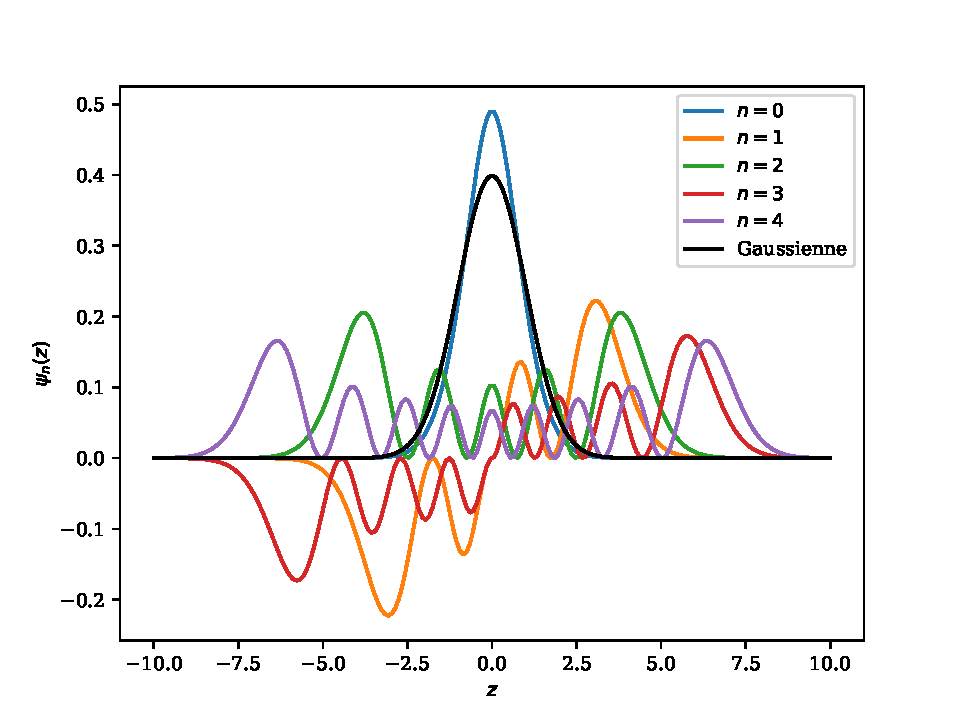
\includegraphics[width=\linewidth]{sosequi-laser/etats-laser.pdf}
	\end{minipage}%
	\begin{minipage}[t]{0.5\linewidth}
    	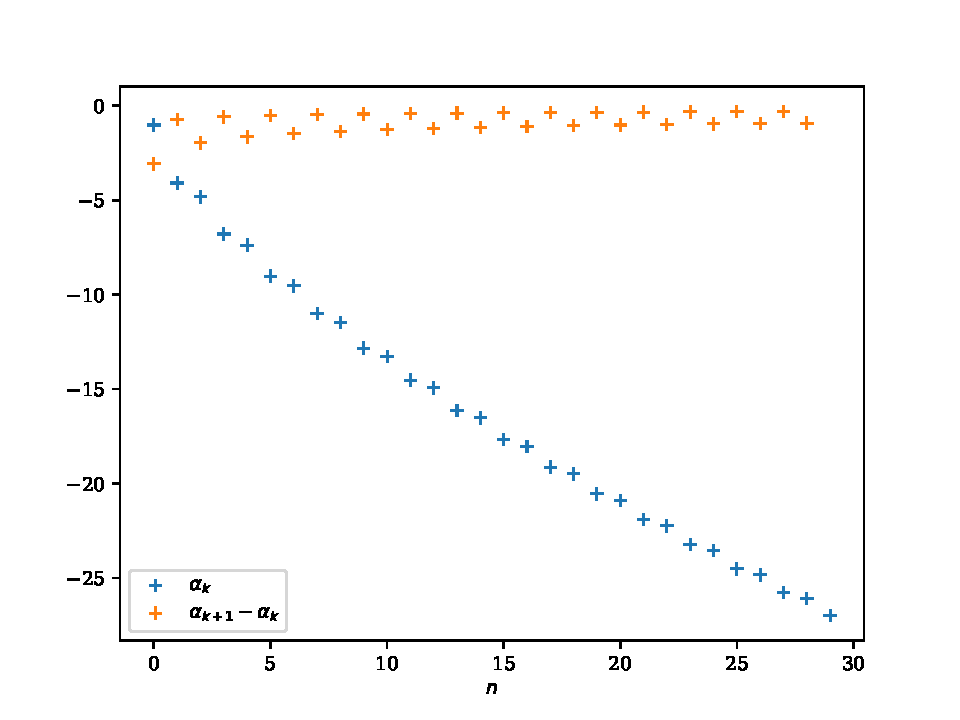
\includegraphics[width=\linewidth]{sosequi-laser/energies-laser.pdf}
	\end{minipage}
    \caption{À gauche, états propres $\psi_n$ avec en noir, une référence par rapport à la distribution gaussienne. À droite, la série $\alpha_n$.}
\end{figure}



On peut adimensionner la distribution des hauteurs par $z = (2\lambda)^\frac{1}{3}h$, et on peut définir une largeur caractéristique de l'interface 
\begin{align}
	\xi_\perp = \frac{1}{(2\beta^2 \sigma B)^\frac{1}{3}}
	\label{xi_perp}
\end{align}


La distribution des hauteurs dans un système infini devient 
\begin{align}
	p(z) = \psi_0^2(z) = \frac{ Ai^2 ( |z|-\alpha_0 )}{ 2 \int_0^\infty dz Ai^2 ( z-\alpha_0 ) }
	\label{airy}
\end{align}
	
\begin{figure}[h]
	\begin{minipage}[t]{0.5\linewidth}
		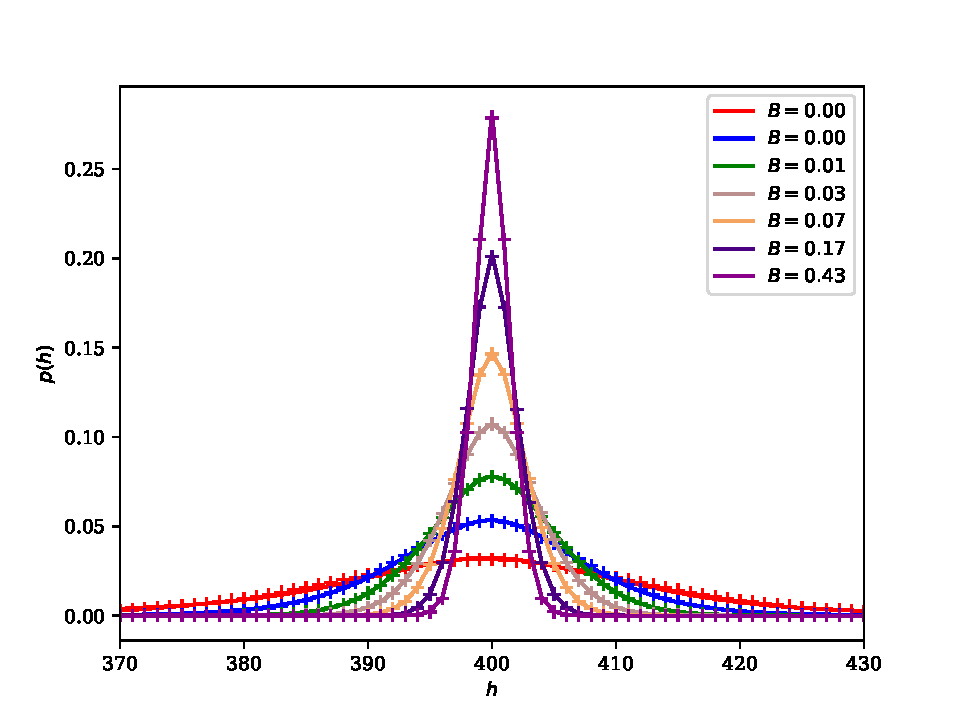
\includegraphics[width=\linewidth]{sosequi-laser/histo.pdf}
	\end{minipage}%
	\begin{minipage}[t]{0.5\linewidth}
		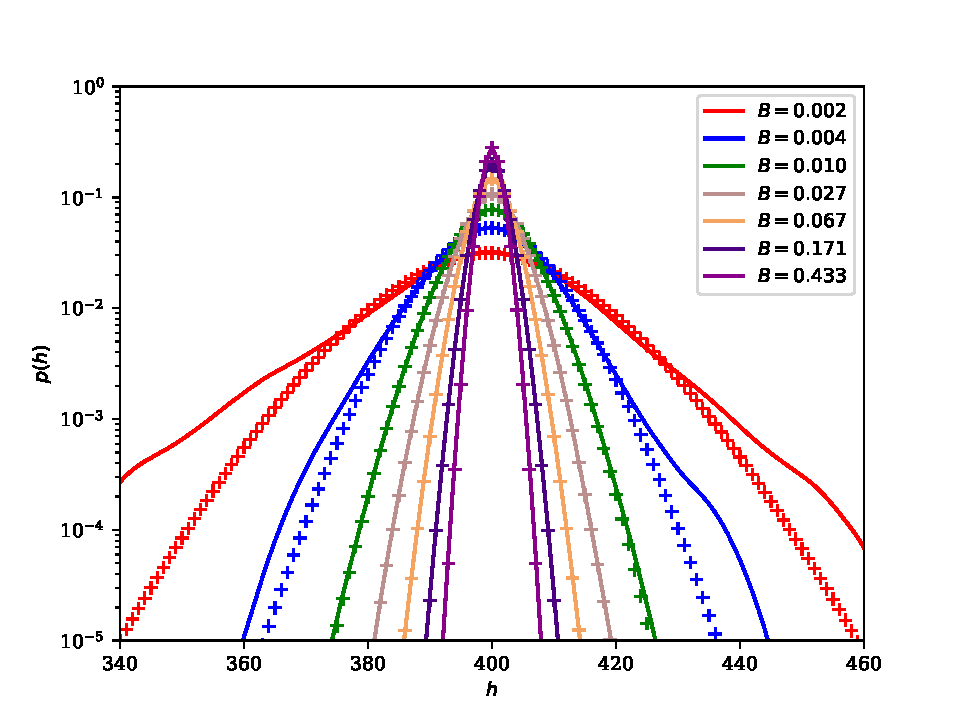
\includegraphics[width=\linewidth]{sosequi-laser/loghisto.pdf}
	\end{minipage}
	\caption{ Distribution de l'interface à $\beta = \beta_C$ autour d'un système centré à $L_Y=400$ en ligne et un fit selon la distribution de Airy \ref{airy}\protect\footnotemark en croix en échelle normale (à gauche) et en échelle log (à droite). Les écarts aux grandes fluctuations sont dues à un temps d’échantillonnage trop faible ($10^8$ MC steps) par rapport au temps de corrélation ($T_{cor} \simeq 100$), ce qui ne donne qu'environ $10^6$ états décorrélés. Par comparaison, à haut champ magnétique, le temps de corrélation est $T_{cor} \simeq 2$.  }
	\label{histo_airy}
\end{figure}

\footnotetext{En C++, les tableaux commençant par l'indice $0$, il est donc plus simple de centrer le système loin de $0$ afin de ne pas avoir à translater les variables à chaque fois. Par ailleurs, le fit est très sensible aux conditions initiales.}

\begin{figure}[h]
	\begin{minipage}[t]{0.5\linewidth}
		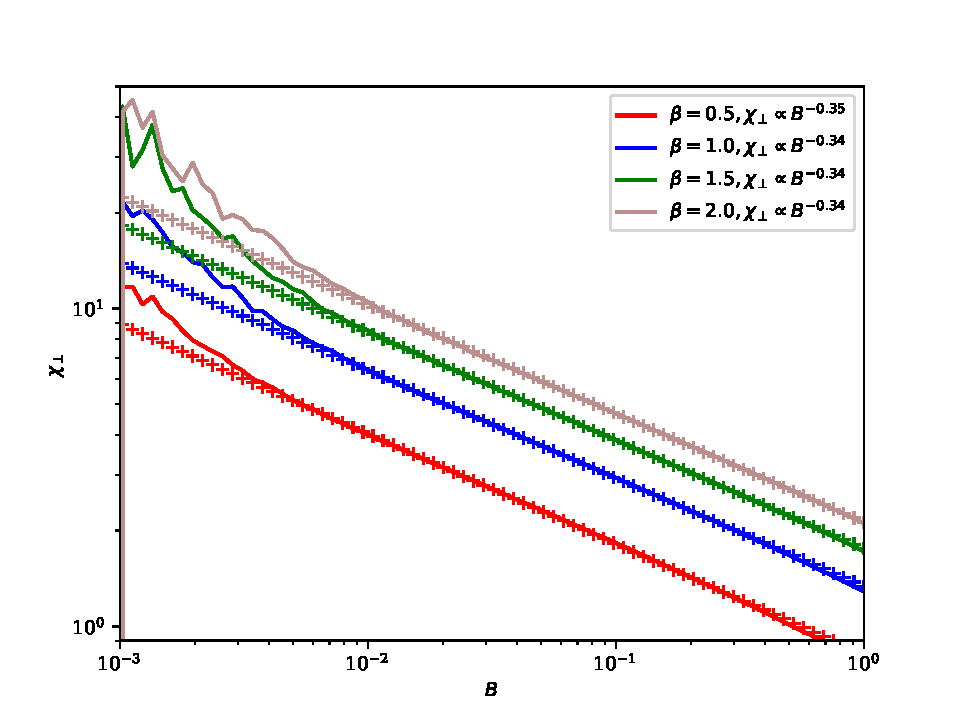
\includegraphics[width=\linewidth]{sosequi-laser/glau-chi.pdf}
	\end{minipage}%
	\begin{minipage}[t]{0.5\linewidth}
		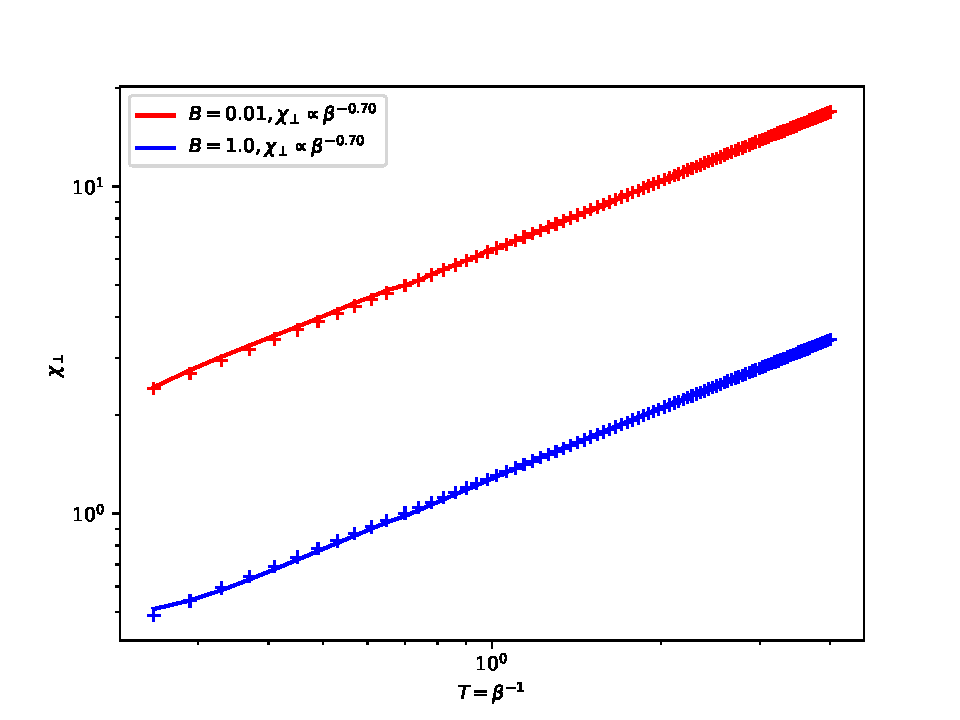
\includegraphics[width=\linewidth]{sosequi-laser/glau-chi-temp.pdf}
	\end{minipage}
	\caption{$\xi_\perp$ calculé via un fit de la distribution numérique par la distribution de Airy après $10^8$ MC steps (\ref{airy}) en fonction du champ magnétique et à température constante (gauche) ou en fonction de la température et à champ magnétique constant (droite). Les fluctuations pour $B$ petit s'expliquent par la difficulté d'équilibrage du système. On retrouve une loi en puissance comme dans l'équation \ref{xi_perp}.}
	\label{expo_airy}
\end{figure}

Comme montré précédemment, le calcul numérique de la distribution de l'interface nous permet d'avoir accès à  la tension de surface de notre modèle via la mesure de la longueur caractéristique $\xi_\perp$. Dans la figure \ref{histo_airy}, le fit de la distribution des hauteurs via l'équation \ref{airy} nous permet d'obtenir $\xi_\perp(\beta,B)$ de la figure \ref{expo_airy}. Ainsi, on obtient que 
\begin{align}
	\xi_\perp(\beta,B) \propto \beta^{-0.34} B^{-0.70} 
\end{align}

\textbf{Est-ce utile de faire une étude plus poussée sur plus de B et $\beta$ afin d'avoir une barre d'erreur sur les exposants ?}

Grâce aux calculs, il est possible d'inverser \ref{xi_perp} afin de trouver numériquement la tension superficielle du système. Dans le tableau \ref{tab_sigma}, en supposant un exposant en $\beta$ de $-0.70$, un tableau à titre informatif sur la tension de surface calculée en fonction de différents paramètres $T = \frac{1}{\beta}$ et $B$ grâce à l'équation \ref{xi_perp}. Les grandes fluctuations de $\sigma$ proviennent d'un échantillonage trop faible du calcul de l'exposant de $\beta$ et de $B$. De plus, d'après la figure \ref{expo_airy}, il semblerait que la loi en puissance ne soit pas valable dans tous les régimes, ce qui ajoute de l'incertitude à nos calculs.
Au final on constate que $\sigma \simeq 4.5$ dans notre modèle pour $J=1$. Des études plus approfondies utilisant la fonction de corrélation et $\xi_\parallel$ permettraient calculer précisément la tension superficielle dans le modèle SOS.

\begin{table}[h]
    \centering
$\begin{array}{|c|c|c|c|c|}
\hline
    T & B & \xi_\perp & \text{Exposant de B} &  \sigma \\
\hline
0.5 & 0.01 & 3.94 & -0.347 & 4.55 \\
0.5 & 1.0 & 0.78 & -0.347 & 4.01 \\
1.0 & 0.01 & 6.29 & -0.340 & 4.80 \\
1.0 & 1.0 & 1.28 & -0.340 & 4.23 \\
1.5 & 0.01 & 8.36 & -0.340 & 4.75 \\
1.5 & 1.0 & 1.72 & -0.340 & 4.36 \\
2.0 & 0.01 & 10.26 & -0.342 & 4.71 \\
2.0 & 1.0 & 2.11 & -0.342 & 4.37 \\
\hline
\end{array}$
    \caption{Meilleure estimation possible de la tension superficielle d'après les simulations numériques pour quelques valeurs de $T$ et de $B$.  }
    \label{tab_sigma}
\end{table}

    \section{Fonction de corrélation }

On peut également calculer la fonction de corrélation à deux-points. 
D'après l'éq \ref{schro_temp}, l'énergie de chaque état est une longueur caractéristique de chaque mode, $E_0$ étant la plus importante contribution au système. La longueur de corrélation parallèle à l'interface étant de l'ordre de grandeur de $E_0^{-1}$, on a 
\begin{align}
	\xi_\parallel = \frac{1}{E_0} =  2^\frac{1}{3}  \beta^{-\frac{1}{3}} \sigma^{-\frac{1}{3}}B^{-\frac{2}{3}}
\end{align}


Dans la limite thermodynamique $L$ grand, la fonction de corrélation  à l'interface est
\begin{align}
	C_f(r) &= \langle f(h(0))f(h(r))\rangle - <f(h(0))><f(h(r))>
\end{align}
Puisque nous sommes dans la limite thermodynamique, la fonction de partition devient $\mZ \simeq e^{-E_0 L}$ et $<f(h(0))> = <f(h(r))> = \int_{-\infty}^\infty dh f(h) \psi_0(h)^2 $.
On obtient alors que
\begin{align}
	C_f(r) =  \sum_{n\neq 0}\left[\int_{-\infty} ^\infty dh\  f(h)\psi_n(h)\psi_0(h)\right]^2\exp(-[\alpha_n-\alpha_0] \frac{r}{\xi_{||}})
\end{align}
En particulier, si
\begin{align}
	f(h) = {\rm sign}(h-y)
\end{align}
alors $C_f(r)=C(y,r)$ est la fonction de corrélation spin-spin mesurée parallèlement à l'interface à la hauteur $y$. On peut décomposer l'intégrale en deux parties, et grâce à un changement de variable obtenir
\begin{align}
	\int_{-\infty} ^\infty dh\  f(h)\psi_n(h)\psi_0(h)=  2\int_y ^\infty dh\  \psi_n(h)\psi_0(h)
\end{align}
Puisque les $\psi_n$ sont des fonctions d'onde orthogonales répondant à l'équation de Schrödinger, l'intégrale pour $n\neq 0$ est
\begin{align}
	I(n,y)&= \int_y^\infty dh\psi_n(h)\psi_0(h)  \nn
	&= \frac{1}{2}\frac{\psi_0(x)\psi'_n(y) - \psi_n(x)\psi_0'(y)}{\epsilon_n-\epsilon_0}
\end{align} 
Comme précédement, on notant $z= \frac{y}{\xi_\perp}$, on simplifie la fonction de corrélation en
\begin{align}
	C(z ,r) = \sum_{n\neq 0} \frac{\left[ Ai(|z|-\alpha_0)Ai'(|z|-\alpha_n) -Ai(|z|-\alpha_n)Ai'(|z|-\alpha_0) \right]^2}
{ \int_0^\infty dz Ai^2 ( z-\alpha_0 )2 \int_0^\infty dz Ai^2 ( z-\alpha_n ) (\alpha_n-\alpha_0)^2}e^{-[\alpha_n-\alpha_0] \frac{r}{\xi_{||}}}
\end{align}

La constante de normalisation peut être encore simplifiée. L'intégration par partie donne
\begin{align}
	N_n = \int_0^\infty dz Ai^2 (z -\alpha_n) = [z Ai^2 (z -\alpha_n)]_0^\infty - 2\int_0^\infty dz  z Ai(z -\alpha_n)Ai'(z -\alpha_n)
\end{align}
Le terme aux limites est nul, et en utilisant l'équation d'Airy 
\begin{align}
	Ai''(z) -z{\rm Ai}(z)=0 \implies z Ai(z-\alpha_n) = Ai''(z-\alpha_n) + \alpha_n Ai(z-\alpha_n)
\end{align}
on obtient
\begin{align}
	N_n &= -2\int_0^\infty dz [Ai''(z -\alpha_n)+\alpha_n Ai(z -\alpha_n)] Ai'(z -\alpha_n)  \nn
	&= Ai'^2(-\alpha_n) + \alpha_n Ai^2(-\alpha_n).
\end{align}

Cela nous donne au final
\begin{align}
	C(z,r) = \frac{1}{6.7 \times 10^{-3}}\sum_{n\neq 0} \frac{\left[ Ai(|z|-\alpha_0)Ai'(|z|-\alpha_n) -Ai(|z|-\alpha_n)Ai'(|z|-\alpha_0) \right]^2}
{(Ai'^2(-\alpha_n) + \alpha_n Ai^2(-\alpha_n))  (\alpha_n-\alpha_0)^2}e^{-[\alpha_n-\alpha_0] \frac{r}{\xi_{||}}}
\end{align}

À grande distance, seul le terme premier état excité $n=1$ contribue à la fonction de corrélation, ce qui nous donne
\begin{align}
C(x,r) \approx \frac{[{\rm Ai}\left(\frac{|x|}{\xi_{\perp}} -\alpha_{0}\right){\rm Ai}'\left( \frac{|x|}{\xi_{\perp}}-\alpha_{1}\right)-{\rm Ai}\left(\frac{|x|}{\xi_{\perp}} -\alpha_{1}\right){\rm Ai}'\left(\frac{|x|}{\xi_{\perp}} -\alpha_{0}\right)]^2}{\left[ {\rm Ai}'^2(-\alpha_{1}) \alpha_0 {\rm Ai}^2(-\alpha_0)\right](\alpha_1-\alpha_0)^2}\exp(-[\alpha_1-\alpha_0] \frac{r}{\xi_{||}}).
\end{align}

This is still quite complicated but if we restrict attention to $x=0$ we find
\begin{align}
C(0,r) \approx \frac{1}{(\alpha_1-\alpha_0)^2\alpha_0}\exp(-[\alpha_1-\alpha_0] \frac{r}{\xi_{||}}).
\end{align}
However at $x=0$ we can actually do better using the boundary conditions
that ${\rm Ai}(-\alpha_{2n+1}) =0$ and ${\rm Ai}'(-\alpha_{2n}) =0$ to give
\begin{align}
C(0,r) = \sum_{n=0}^\infty \frac{1}{(\alpha_{2n+1}-\alpha_0)^2\alpha_0}\exp(-[\alpha_{2n+1}-\alpha_0] \frac{r}{\xi_{||}}).%
\end{align}
We know that $C(0,0)=1$ and so (unless there is a mistake in the calculations) we have the remarkable identity
\begin{align}
\sum_{n=0}^\infty \frac{1}{(\alpha_{2n+1}-\alpha_0)^2\alpha_0} = 1.
\end{align}

The above calculation has some strange consequences, we see that for all $x$ the correlation function for large $r$ 
decays as 
\begin{align}
A(\frac{x}{\xi_\perp})\exp(-[\alpha_1-\alpha_0] \frac{r}{\xi_{||}}),
\end{align}
where $A(x)$ is the $x$ dependent amplitude, so the correlation length at large $r$ is independent of the position
$x$, now going into the bulk this predicts that $\xi_{||} = \xi_b$ where $\xi_b$ is the bulk correlation length (but in the presence of the magnetic field). 


\begin{figure}[h]
	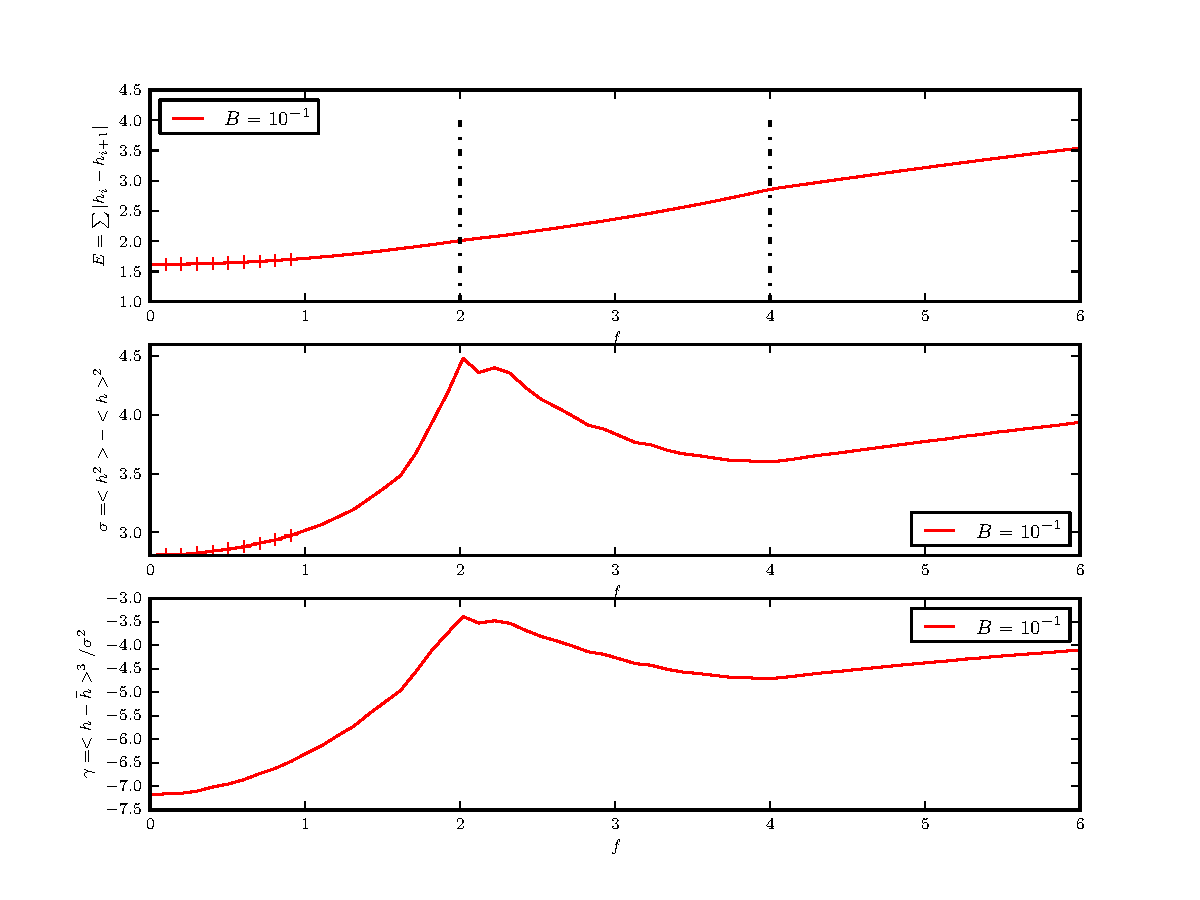
\includegraphics[width=\linewidth]{./sosequi-laser/sosj1.pdf}
	\caption{Énergie $E= \langle \sum_i |h_i-h_i+1| \rangle$ (en pointillé sa dérivée), variance $\sigma = \langle (H - \langle H \rangle )^2  \rangle$ et asymétrie $\gamma = \langle (H - \langle H \rangle )^3  \rangle / \sigma^2$ pour $B^0.1$. La magnétisation est constante et égale à $\langle H \rangle = 4.51$. Le temps de corrélation du système est presque constant en fonction du cisaillement $f$, allant de  $\tau(f=0) = 5.04$ à $\tau(f=6) = 5.00$ étapes de Monte Carlo. On note une brisure à $f=2J$ et $f=4J$.
Les croix notent un fit en carré pour petit $f$, montrant la symétrie du système par inversion du signe de $f$. }
\end{figure}

\begin{figure}
	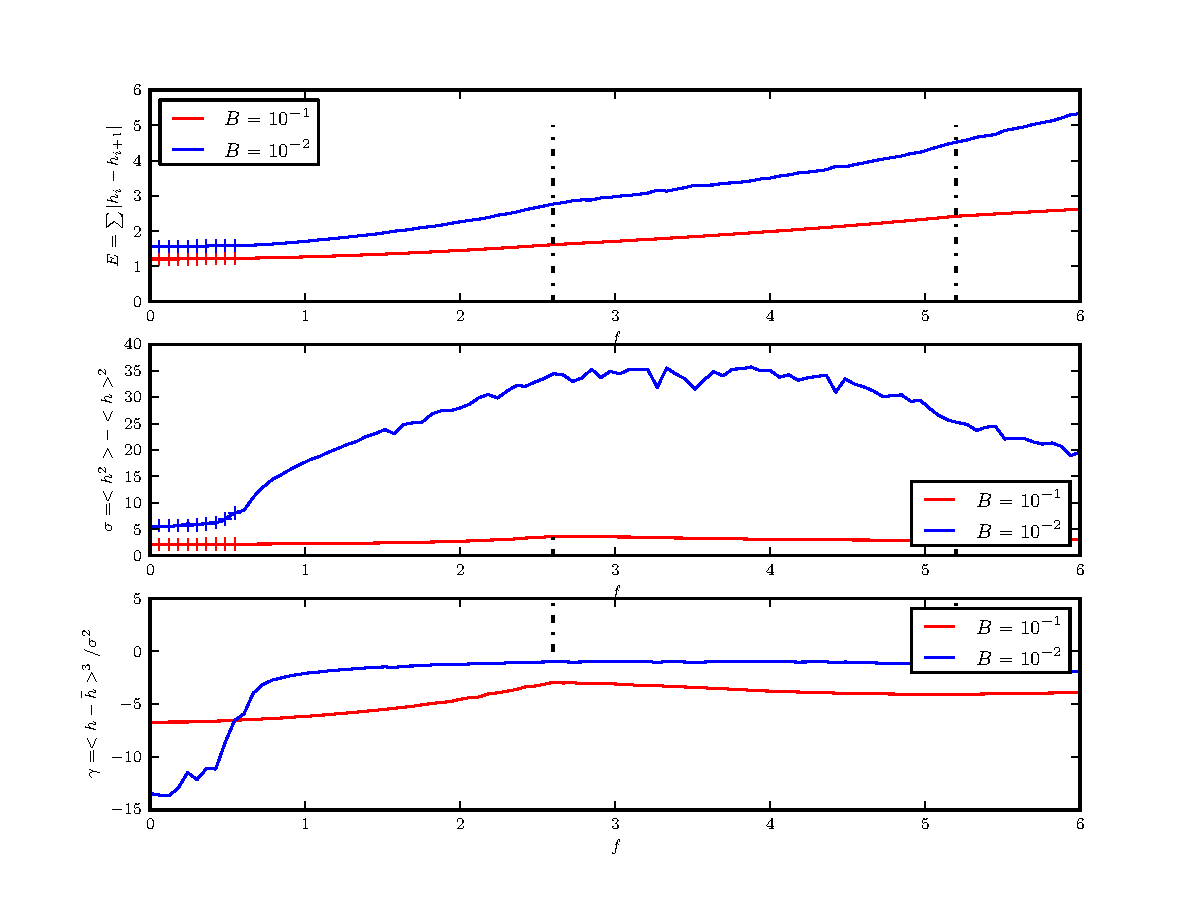
\includegraphics[width=\linewidth]{./sosequi-laser/j13.pdf}
	\caption{Same as before, with $J=1.3$ We observe a net inflexion in the energy at $2 J$ for  $B=0.01$ which corresponds to $<H>=11$. Nvertheless there is not threshold at $4 J = 5.2$. My guess is that the system is too far away from the boundary in order to interact strongly with it. Interstingly enough, for $B=0.1$, $<H>=3$ and we are too close to the boundaries to see anything.}
\end{figure}


\section{Cisaillement avec deux types de particules}

La construction naïve d'un modèle continu du cisaillement avec un seul type de particules ne donnera aucun résultat. En effet, pour que le cisaillement induise des effets hors équilibre, il faut que la dynamique des particules dans tout repère galilén soit le même. Si l'on considère une force de cisaillement uniforme qui induit la même vitesse moyenne sur toutes les particules du système, en nous plaçant dans un repère bougeant à la même vitesse que cette vitesse moyenne, nous retrouvons les mêmes propriétés à l'équilibre.
Afin de briser la symmétrie de translation, il faut soit induire un cisaillement non-uniforme, soit introduire des particules qui réagissent de manière différente vis-à-vis de cette force. Dans notre exemple sur les colloïdes, la gravité agit bien sur les polymères mais bien moins sur le solvant, ce qui brise en effet l'invariance galiléenne. 
Plusieurs études récentes portent sur le mouvement de systèmes avec plusieurs particules browniennes, incluant le problème des électrolytes étudié par Onsager \cite{onsager} il y a longtemps.

	\subsection{Discussion about the Gaussian model}
	
The Gaussian model has a stronger interaction, been as
\begin{align}
	\Delta E = J \sum (h'_i-h'_{i+1})^2 -(h_i-h_{i+1})^2+ f (i-j)
\end{align}
In this model the bond energy between two microstates can take any integer, as 
\begin{equation*}
	(h_i-h_j+2)^2 - (h_i-h_j)^2 = 4 (h_i-h_j+1)
\end{equation*}

The gaussian interaction is very strong, so we could expect a very smooth interface. The mean difference between two sites should be about $h_i-h_{i+1} \simeq 1$. In that case, the energy difference is discretized as ${-8,-4,0,4,8}$. 
Nonetheless we cannot predict exactly the same behaviour as in the SOS model because this approximation has to be verified everytime, which is false. 1

\begin{figure}
	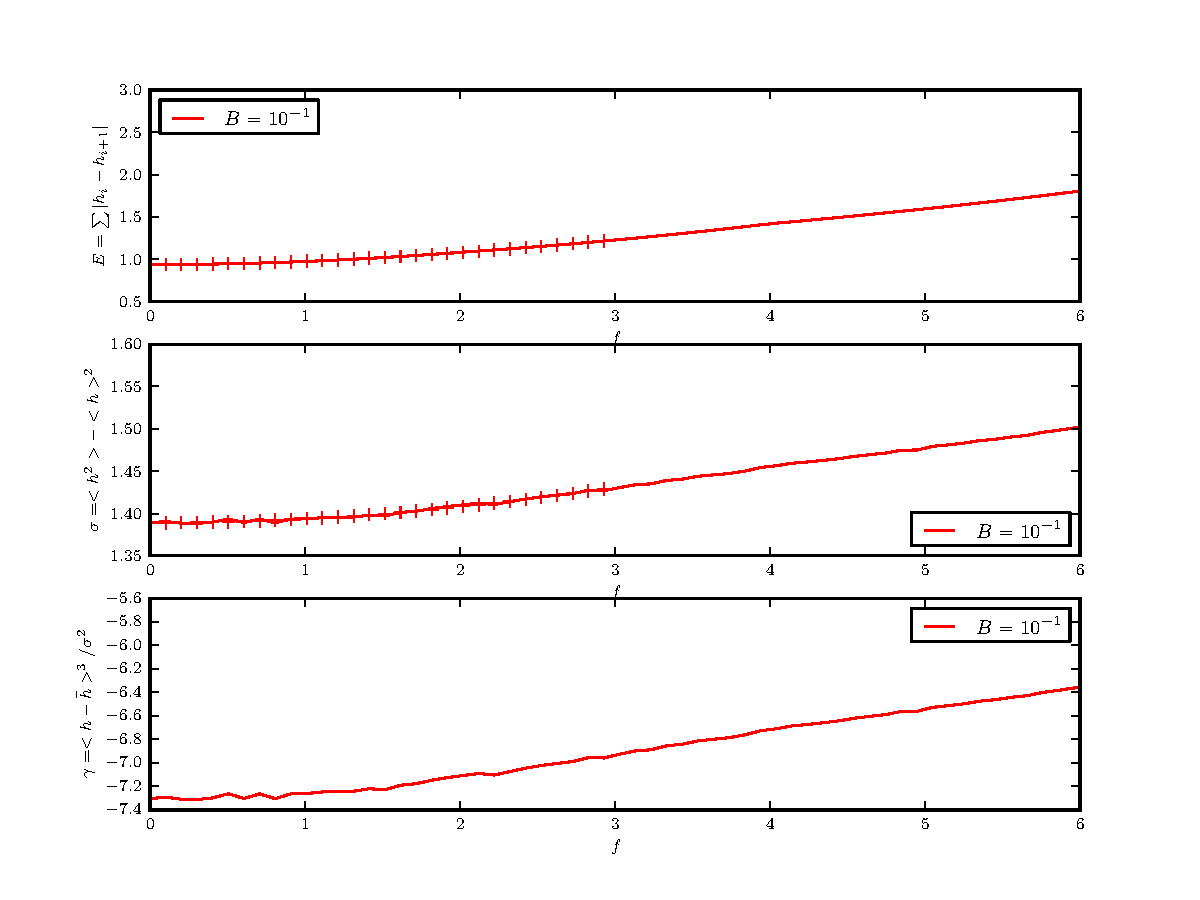
\includegraphics[width=\linewidth]{./sosequi-laser/gauss0.pdf}
	\caption{Bond energy, thickness (variance) and skewness of the interface for two different magnetic pressures. The magnetisation is constant and is equal to $<H>=2$ for $B=0.1$. As we are very close to the boundary, we see no threshold with the drive force. Simulations take longer with this model because the interaction is stronger}
\end{figure}


    \section{Conclusion}

Peu d'études permettent de relier les propriétés macroscopiques d'un système à sa dynamique moléculaire. Dans ce chapitre, nous avons réussi à calculer, via différentes méthodes, l'adéquation entre la théorie et un système discret que l'on a pu simuler. Un fit de nos données a permis de relever une valeur pour la tension superficielle pour le modèle SOS avec un hamiltonien gaussien et un champ magnétique agissant comme un laser. 
%\chapter{A+B POP model : la totale}
\label{chap-article-dean}

Précédement, nous avons vu que l'écoulement injectée de l'énergie dans l'interface ne peut y être dissipée par des mécanismes d'évaporation, augmentant ainsi la largeur moyenne de l'interface. Nous avons également utilisé la présence de plusieurs types de particules afin de briser l'invariance par translation dans un repère galiléen par rapport à la vitesse moyenne induite par l'écoulement uniforme afin d'étudier les statistiques hors-équilibre.

Grâce à l'approche par la fonctionnelle de densité stochastique (SDFT) \cite{dean1996}, nous étudions dans ce chapitre la possibilité de dispersion de l'énergie injectée par l'écoulement, et nous expliquons analytiquement pourquoi l'interface devient plus rigide.
Afin de simplifier un peu les équations, nous allons supposer deux champs suivant le modèle C (selon la classification de Hohenberg et Halperin\cite{hohenberg_theory_1977}). D'un côté nous avons les colloïdes, représentés par un champs possèdant une dynamique conservée et se déplaçant à vitesse constante. De l'autre côté nous avons un couplage avec un réservoir d'un solvant. 

    \section{Le modèle C=A+B}
    
Soient deux champs scalaires $\psi$ et $\phi$ représentant les valeurs moyennes mésoscopiques de deux types de particules différentes. On suppose que le système possède deux phases stables avec une concentration moyenne du champ $\phi(\vec{x})$ données par $\psi_1$ et  $\psi_2$, la différence du paramètre d'ordre entre les deux phases étant $\Delta\psi= \psi_2 -\psi_1\greater 0$. On suppose également que $\phi(\vec{x},z\rightarrow -\infty)=\psi_2$ et $\phi(\vec{x},z\rightarrow \infty)=\psi_1$. On décompose l'hamiltonien deux parties, 
\begin{align}
    H[\psi,\phi] = H_1[\psi] +H_2[\psi,\phi]
\end{align}
Le premier Hamiltonien $H_1$, de la forme Landau-Ginzburg, correspond à l'énergie total du système
\begin{align}
    H_1[\psi]=\int d\vec{x}\left[\frac{\kappa}{2}[\nabla\psi(\vec{x})]^2 + V(\psi(\vec{x}))- gz \psi(\vec{x})\right].
\end{align}
où le premier terme représente la tension de surface et le troisième terme représente l'énergie due à la gravité. Ce même terme permet d'introduire une longueur de corrélation finie entre les deux phases. 

\begin{figure}
    \centering
    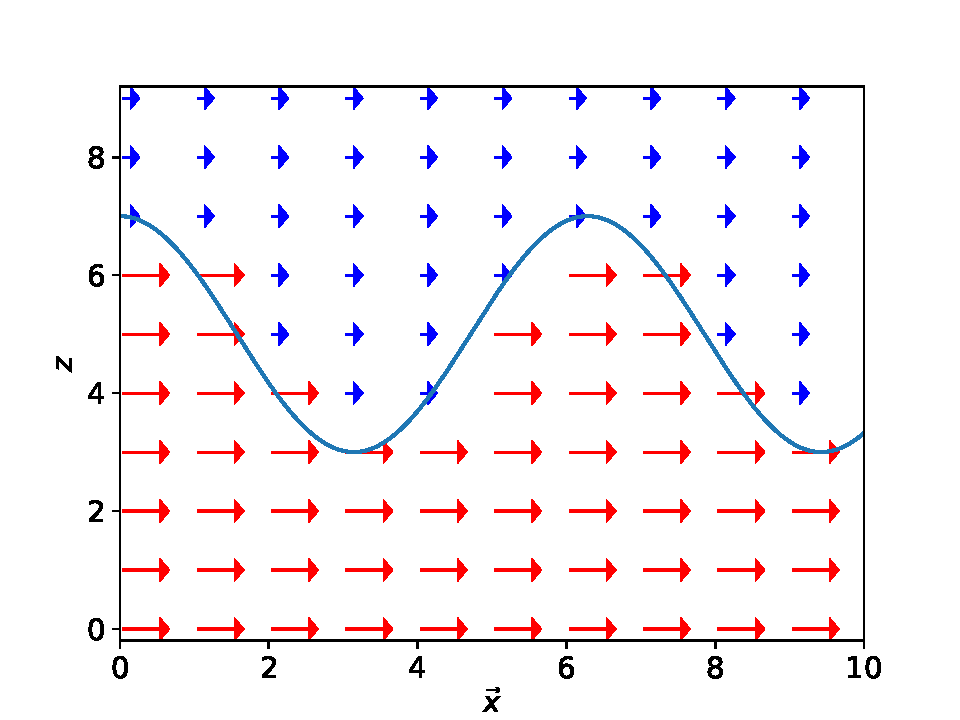
\includegraphics[width=0.5\linewidth]{pop/ab-phi.pdf}
    \caption{Schéma d'un écoulement uniforme parallèle à l'interface dépendant de la phase. Ici, on prend un modèle d'interface \ref{ab-interface} avec $\psi(\vec{x})=\psi_2$ en dessous de linterface et $\phi(\vec{x})=\psi_1$ au dessus. }
\end{figure}

Le second Hamitlonien $H_2$ est pris pour un couplage quadratique entre les deux champs
\begin{equation}
H_2 =\int d\vec{x} \frac{\lambda}{2}(1-\psi(\vec{x})-\phi(\vec{x}))^2,
\end{equation}
où l'on considère la conservation du volume totale des fractions des phases. Le champ $\phi$ peut se comprendre comme la fraction volumique locale d'un solvant d'un système de colloïdes. L'objectif de ce champ est de proposer des particules qui ne sont pas concernées par l'écoulement, peut-être parce qu'elles bougent à une échelle de temps bien plus longue. La présence de ce champ ne change cependant rien aux propriétés à l'équilibre du champ de colloïdes $\psi$. 
L'ajout de ce champ couplé permet de supprimer l'invariance galiléenne par rapport à la vitesse moyenne provoquée par l'écoulement. 

La fonction de partition s'écrit 
\begin{equation}
Z = \int d[\phi]d[\psi]\exp(-\beta H_1[\psi]- \beta H_2[\psi,\phi]) = CZ_{eff},
\end{equation}
{\color{red} expliciter l'étape d'intégration}
où $Z_{eff}$ est une fonction de partition effective ne dépendant que du champ $\psi$.
is the effective partition function for the field $\psi$, after we have integrated out the degrees of freedom corresponding to the field $\phi$,
and $C$ is a constant term resulting from this integration. The effective partition function is thus simply given by

La nouvelle fonction de partition est alors 
\begin{equation}
    Z_{eff} = \int d[\psi]\exp(-\beta H_1[\psi]),
\end{equation}
Comme expliqué plus haut, on voit que le champ $\phi$ n'a plus aucun effet sur les propriétés statistiques à l'équilibre du champ $\psi$.


On considère maintenant la dynamique de schamps. On prend la modèle de diffusivité local (modèle B selon la classification d'Hohenberg et Halpering) pour le champ $\psi$ tandis que l'on prend un modèle non conservé (modèle A) pour le solvant $\phi$.
\begin{align}
    \frac{\partial \psi(\vec{x},t)}{\partial t} +\vec{v}\cdot \vec{ \nabla}\psi(\vec{x},t)&= D\nabla^2\frac{\delta H}{\delta \psi(\vec{x})}+ \sqrt{2D T}\nabla \cdot {\bm \eta}_1(\vec{x},t) \\
    \frac{\partial \phi(\vec{x},t)}{\partial t} &= -\alpha\frac{\delta H}{\delta \phi(\vec{x})}+ \sqrt{2\alpha T}{ \eta}_2(\vec{x},t).
\end{align}
La première équation correspond à une diffusivitié locale $D$ et un terme d'advection par une champ de vitesse contstant $\vec{v}$ . La seconde équation correspond juste à l'équation du modèle A, avec un coefficient cinétique $\alpha$ correspondant au temps de relaxation du système vers l'équilibre. 


The second equation has no advection term and is simple model A dynamics. In principle we can also treat the case where the dynamics of the field $\phi$ is also diffusive and thus of model $B$ type, the analysis given here can be extended to this case but the analysis of the resulting equations is considerably more complicated. The use of model A dynamics for the solvent is justified by assuming that its dynamics is faster than that of the colloids and that the volume fraction can vary due to local conformational changes rather than  diffusive transport.

The noise terms above 
are uncorrelated and Gaussian with zero mean, their correlation functions are given by
\begin{eqnarray}
\langle \eta_{1i}(\vec{x},t) \eta_{1j}(\vec{x}',t)\rangle&=& \delta_{ij}\delta(t-t') \delta(\vec{x}-\vec{x}') \\
\langle \eta_{2}(\vec{x},t) \eta_{2}(\vec{x}',t)\rangle&=& \delta(t-t') \delta(\vec{x}-\vec{x}') ,
\end{eqnarray}
and $T$ is the temperature in units where $k_B=1$.
These dynamical equations  are thus explicitly given by
\begin{equation}
\frac{\partial \psi(\vec{x},t)}{\partial t} +\vec{v}\cdot { \nabla}\psi(\vec{x},t)= D\nabla^2[\frac{\delta H_1}{\delta \psi(\vec{x})}+\lambda(\phi(\vec{x},t) + \psi(\vec{x},t))]+ \sqrt{2D T}\nabla \cdot {\boldsymbol \eta}_1(\vec{x},t)
\end{equation}
and
\begin{equation}
\frac{\partial \phi(\vec{x},t)}{\partial t} = -\alpha\lambda[\phi(\vec{x},t) + \psi(\vec{x},t)]+ \sqrt{2\alpha T}{ \eta}_2(\vec{x},t).
\end{equation}
Taking the temporal Fourier transform, defined with the convention
\begin{equation}
\tilde F(\vec{x}, \omega) = \int_{-\infty}^\infty dt \exp(-i\omega t)F(\vec{x}, t),
\end{equation}
we can eliminate the field $\tilde \phi$ which is given by
\begin{equation}
\tilde \phi(\vec{x},\omega) = \frac{-\alpha\lambda \tilde \psi(\vec{x},\omega)+\sqrt{2\alpha T}\tilde \eta_2(\vec{x},\omega)}{i\omega +\alpha \lambda},
\end{equation}
this then gives the closed equation for $\tilde \psi$:
\begin{equation}
\left[1-\frac{\lambda D \nabla^2}{i\omega+\alpha\lambda}\right]i\omega \tilde\psi(\vec{x}, \omega) +\vec{v}\cdot\nabla\tilde\psi(\vec{x}, \omega)
= D\nabla^2 \tilde \mu(\vec{x},\omega) +  \tilde \zeta(\vec{x},\omega),
\end{equation}
where 
\begin{equation}
\mu(\vec{x},t)=\frac{\delta H_1}{\delta \psi(\vec{x},t)}
\end{equation}
is the effective chemical potential associated with the field $\psi$ and the noise term is given by
\begin{equation}
\tilde \zeta(\vec{x},\omega) = \frac{\sqrt{2\alpha T}D\lambda}{i\omega + \alpha\lambda}\nabla^2\tilde \eta_2(\vec{x},\omega) +
\sqrt{2DT}\nabla\cdot\tilde {\bm \eta}_1(\vec{x},\omega).
\end{equation}
Inverting the temporal Fourier transform then gives the effective evolution equation
\begin{equation}
\frac{\partial \psi(\vec{x},t)}{\partial t} -\lambda D\nabla^2\int_{-\infty}^t dt'
\exp(-\alpha\lambda(t-t')) \frac{\partial \psi(\vec{x},t')}{\partial t}+\vec{v}\cdot\nabla\psi(\vec{x}, t)=D\nabla^2  \mu(\vec{x},t') +  \zeta(\vec{x},t).\label{dyn1}
\end{equation}
\section{Effective interface dynamics}
We now follow the method of \cite{bray2001,bray2002} to derive the dynamical equation  for the interface between the two phases. It is assumed that the driving is in the ${\bf r}=(x,y)$ plane and that the system varies from phase $1$ to phase $2$ in the $z$ direction. The dynamical evolution for the field $\psi$ in Eq. (\ref{dyn1}) is first written as
\begin{equation}
\nabla^{-2}\left[\frac{\partial \psi(\vec{x},t)}{\partial t}+\vec{v}\cdot\nabla\psi(\vec{x}, t)\right] -\lambda D\int_{-\infty}^t dt'
\exp(-\alpha\lambda(t-t')) \frac{\partial \psi(\vec{x},t')}{\partial t'}=D  \mu(\vec{x},t') + \nabla^{-2} \zeta(\vec{x},t).\label{eqpsi}
\end{equation}
We now assume that the field $\psi$ can be written in the form
\begin{equation}
\psi(\vec{x},t) = f(z-h({\bf r},t)),
\end{equation}
and $f(z)\to \psi_2$ as $z\to -\infty$ and $f(z)\to \psi_2$ as  $z\to \infty$.
We now note the following results
\begin{eqnarray}
\frac{\partial f(z-h({\bf r},t))}{\partial t} &=& -f'(z-h({\bf r},t))\frac{h({\bf r},t)}{\partial t}\\
\nabla f(z-h({\bf r},t) )&=& [{\bf e}_z -\nabla h({\bf r},t)]f'(z-h({\bf r},t))]\\
\nabla^2 f(z-h({\bf r},t)) &=& f''(z-h({\bf r},t)[1 + [\nabla h({\bf r},t)]^2] -\nabla^2 h({\bf r},t)f'(z-h({\bf r},t)),
\end{eqnarray}
and thus we find
\begin{equation}
\mu(\vec{x},t)= -\kappa\left(f''(z-h({\bf r},t)[1 + \nabla^2 h({\bf r},t)] -\nabla^2 h({\bf r},t)f'(z-h({\bf r},t))\right) + V'(f(z-h({\bf r},t)) - gz .
\end{equation}
Multiplying both sides of the above by $f'(z-h({\bf r},t))$ yields
\begin{eqnarray}
&&f'(z-h({\bf r},t))\mu(\vec{x},t)=\nonumber \\
 &&-\kappa\left(f'(z-h({\bf r},t)f''(z-h({\bf r},t)[1 + \nabla^2 h({\bf r},t)] -\nabla^2 h({\bf r},t)f'(z-h({\bf r},t))^2\right) + V'(f(z-h({\bf r},t))f'(z-h({\bf r},t))\nonumber \\
 &&- gz f'(z-h({\bf r},t)) \nonumber
\end{eqnarray}
and then integrating over $z$ we obtain
\begin{eqnarray}
\int_{-\infty}^\infty dz f'(z-h({\bf r},t)\mu(\vec{x},t)&=& \kappa \nabla^2 h({\bf r},t)\int_{-\infty}^\infty dz\ f'(z-h({\bf r},t))^2 - \int_{-\infty}^\infty dz gz f'(z-h({\bf r},t))\nonumber \\&=&
\kappa\nabla^2 h({\bf r},t)\int_{-\infty}^\infty dz'\ f'(z')^2 - \int_{-\infty}^\infty dz' g(z' +h({\bf r},t)) f'(z')\nonumber \\
&=& \kappa\nabla^2 h({\bf r},t)\int_{-\infty}^\infty dz' \ f'(z')^2 -\Delta\psi g h({\bf r},t).
\end{eqnarray}
In the above we have assumed that $\int_{-\infty}^\infty dz' z'f'(z')=0$ by symmetry (this is also consistent with the approximation made later on in Eq. (\ref{eqdelta})). Furthermore one can show that \cite{bray2001,bray2002}
\begin{equation}
\kappa\int_{-\infty}^\infty dz' \ f'(z')^2 = \sigma,\label{mfsig}
\end{equation}
where $\sigma$ is the mean-field equilibrium Cahn-Hilliard estimate of the surface tension, obtained by  assuming that $f(z)=\psi_{MF}(z)$ is the equilibrium mean field profile of the field 
$\psi$. We thus find
\begin{equation}
\int_{-\infty}^\infty dz f'(z-h({\bf r},t)\mu(\vec{x},t) = \sigma[\nabla^2 h({\bf r},t)-m^2 h({\bf r},t)]
\end{equation}
where $m^2 = \Delta\psi g /\sigma$. We now carry out the same operation on the left hand side of Eq. (\ref{eqpsi}). First we have
\begin{eqnarray}
\nabla^{-2}\frac{\partial \psi(\vec{x},t)}{\partial t}&+&\vec{v}\cdot\nabla \psi(\vec{x},t) +\lambda D\int_{-\infty}^t dt'
\exp(-\alpha\lambda(t-t')) \frac{\partial \psi(\vec{x},t')}{\partial t'} = \nonumber \\ 
&-&\nabla^{-2}f'(z-h({\bf r},t))[\frac{\partial h({\bf r},t)}{\partial t} +\vec{v}\cdot\nabla h({\bf r},t)]  +\lambda D\int_{-\infty}^t dt'
\exp(-\alpha\lambda(t-t')) f'(z-h({\bf r},t'))\frac{\partial h({\bf r},t')}{\partial t'}\nonumber \\
&\approx& -\nabla^{-2}f'(z) [\frac{\partial h({\bf r},t)}{\partial t} +\vec{v}\cdot\nabla h({\bf r},t)] +\lambda D\int_{-\infty}^t dt'
\exp(-\alpha\lambda(t-t')) f'(z)\frac{\partial h({\bf r},t')}{\partial t'},\end{eqnarray}
where in the last line above we have neglected terms quadratic in $h$. 
Note that the neglecting of these additional terms is not strictly justified, they could potentially induce non-perturbative effects which render the surface fluctuations non-Gaussian. However we see here that the first order computation we carry out tends to reduce fluctuations with respect to equilibrium or non-driven interfaces and so if the equilibrium theory can be described by an equation which is linear in height fluctuations, it seems physically reasonable to assume that the the approximation also holds for the driven interface. 
Again, we multiply the above by $f'(z)$ and integrate over $z$. In the first term we make use of the approximation
\begin{equation}
f'(z)=\Delta\psi \delta(z)\label{eqdelta}
\end{equation}
and in the second we use the relation in Eq. (\ref{mfsig}). Putting this all together we obtain
\begin{equation}
\Delta\psi^2 \int d{\bf r} G(0,{\bf r}-{\bf r}') [\frac{\partial h({\bf r},t)}{\partial t} +\vec{v}\cdot\nabla h({\bf r},t)] +\frac{\sigma\lambda D}{\kappa}\int_{-\infty}^t dt'
\exp(-\alpha\lambda(t-t'))\frac{\partial h({\bf r},t')}{\partial t'}
= \sigma[\nabla^2 h({\bf r},t)-m^2 h({\bf r},t)] + \xi({\bf r},t),\label{em}
\end{equation}
where $G= -\nabla^{-2}$, or more explicitly
\begin{equation}
\nabla^2 G(z-z',{\bf r}-{\bf r}') = -\delta(z-z') \delta({\bf r}-{\bf r'}).
\end{equation}
The noise term $\xi$ is given by
\begin{equation}
\xi({\bf r},t) = \int_{-\infty}^{\infty} dz f'(z-h({\bf r},t)) \nabla^{-2} \zeta(\vec{x},t).
\end{equation}
Now, as the equations of motion have been derived to first order in $h$ and we wish to recover the correct equilibrium statistics for the non-driven system, we ignore the $h$ dependence in the noise and make the approximation
\begin{equation}
\xi({\bf r},t) \approx \int_{-\infty}^{\infty} dz f'(z) \nabla^{-2} \zeta(\vec{x},t).
\end{equation}
The correlation function of this noise is most easily evaluated in terms of its Fourier transform with respect to  space and time  defined by
\begin{equation}
\hat F({\bf q},\omega)=\int dt d{\bf r}\exp(-i\omega t -i{\bf q}\cdot{\bf r}) F({\bf r},t).
\end{equation}
Using the relations Eqs. (\ref{mfsig}) and (\ref{eqdelta}) one  can show that
\begin{equation}
\langle \hat \xi({\bf q},\omega)\hat \xi({\bf q}',\omega')\rangle 
=2T(2\pi)^d \delta(\omega +\omega') \delta({\bf q}+{\bf q}') \left[
\frac{\sigma}{\kappa}\frac{\alpha D^2\lambda^2}{\omega^2 +\alpha^2\lambda^2} + \frac{D\Delta\psi^2}{2q}\right].
\end{equation}
In full Fourier space the equation of motion for the field $\psi$ then reads
\begin{equation}
\left[i(\omega+{\bf q}\cdot\vec{v})\frac{\Delta\psi^2}{2q} + \frac{D\sigma\lambda}{\kappa} \frac{i\omega}{\alpha\lambda+i\omega}\right] \hat h({\bf q},\omega)= -D\sigma(q^2+m^2)\hat h({\bf q},\omega)+ \hat\xi({\bf q},\omega).\label{dyn}
\end{equation}

From this, the full Fourier transform of the correlation function of the interface height is given by
\begin{equation}
\hat C({\bf q},\omega)  = 2TD \frac{\left[ \frac{\Delta\psi^2}{2q}(\omega^2+\alpha^2 \lambda^2) + \frac{\sigma\alpha D\lambda^2}{\kappa}\right]}{\left|i[\frac{\alpha\lambda\Delta\psi^2}{2 q}(\omega + {\bf q}\cdot\vec{v}) + \frac{\lambda \sigma D}{\kappa}\omega + D\sigma(q^2+m^2)\omega]
+[\alpha\lambda D\sigma(q^2+m^2) -\frac{\Delta\psi^2}{2q}\omega(\omega+{\bf q}\cdot\vec{v})]\right|^2}.
\end{equation}
Using the above we can extract the equal time height-height correlation function in the steady states. Its spatial Fourier transform can shown to be given by
\begin{eqnarray}
\tilde C_s({\bf q}) &=& \frac{1}{2\pi} \int d\omega \hat C({\bf q}, \omega)\nonumber\\
&=&T \frac{\left(2 D\sigma q(\kappa[q^2+m^2]+\lambda)+\alpha\kappa\lambda\Delta\psi^2\right)^2 +\kappa^2 \Delta\psi^4 ({\bf q}\cdot\vec{v})^2}{\sigma[q^2+m^2]\left(2D q\sigma (\kappa[q^2+m^2]+\lambda)+\alpha \kappa\lambda \Delta\psi^2\right)^2 + \kappa\left(\kappa\sigma[q^2+m^2] + \lambda\sigma\right)\Delta\psi^4({\bf q}\cdot\vec{v})^2}.\label{eqmaind}
\end{eqnarray}
An outline of the derivation of this result is given in the Appendix to the paper.
In the absence of driving, {\em i.e.} when $\vec{v}={\bf 0}$ we recover the equilibrium correlation function
\begin{equation}
\tilde C_s({\bf q})= \tilde C_{eq}({\bf q})= \frac{T}{\sigma[q^2+m^2]},
\end{equation} 
here we see that  $1/m= \xi_{eq}$ is the so called capillary length, which is the equilibrium correlation length of the height fluctuations. We also notice that the correlation function for wave vectors perpendicular to the driving direction is simply the equilibrium one.

If we write $C_s({\bf q})= T/H_s({\bf q})$ we can interpret $H_s({\bf q})$ as an effective quadratic Hamiltonian for the height fluctuations, it is thus given by
\begin{equation}
H_s({\bf q}) = \sigma[q^2+m^2] + \frac{\kappa\lambda\sigma \Delta\psi^4 ({\bf q}\cdot\vec{v})^2}{\left(2 D\sigma q(\kappa[q^2+m^2]+\lambda)+\alpha\kappa\lambda\Delta\psi^2\right)^2 +\kappa^2 \Delta\psi^4 ({\bf q}\cdot\vec{v})^2}
\end{equation}
For small $q$ we find 
\begin{equation}
H_s({\bf q}) = \sigma m^2 + \sigma q^2(1+ \frac{v^2\cos^2(\theta)}{\alpha^2\lambda\kappa}),
\end{equation}
where $\theta$ is the angle between the wave vector ${\bf q}$ and the direction of the driving. 
This thus gives a direction dependent surface tension 
\begin{equation}
\sigma_s(\theta) = \sigma(1+ \frac{v^2\cos^2(\theta)}{v^2_0}),
\end{equation}
where we have introduced the intrinsic velocity $v_0 = \sqrt{\alpha^2\lambda\kappa}$ which depends on the microscopic {\em dynamical} quantity $\alpha$ associated with the model A dynamics of the field $\phi$, as well as the microscopic static quantities $\kappa$ (which generates the surface tension) and $\lambda$ the coupling between the field $\psi$ and $\phi$. This appearance of dynamical and static quantities that are otherwise hidden in equal time correlation functions in equilibrium is already implicit in the works of Onsager \cite{hem1996} where it is used to compute the conductivity of Brownian electrolytes and the explicit expressions were derived using stochastic density functional theory in \cite{dem2016}. We also note that the universal thermal Casimir effect between model Brownian electrolyte systems  driven by an electric field 
exhibits similar features, developing a dependency on both additional static and dynamical variables with respect to the equilibrium case \cite{dean2016}


However for this small $q$ expansion we see that the microscopic 
quantities $D$, the diffusion constant of the field $\phi$, and the order parameter jump
$\Delta\psi$ do not appear. 

From the above, we see that  in the direction of the driving the surface tension increases and the fluctuations of the surface are thus suppressed. We may also write 
\begin{equation}
H_s({\bf q}) = \sigma_s(\theta) [q^2 + m^2_e(\theta)],
\end{equation}
with 
\begin{equation}
m^2_s(\theta) =\frac{ m^2}{1+ \frac{v^2\cos^2(\theta)}{v_0^2}},
\end{equation}
this corresponds to a correlation length 
\begin{equation}
\xi_s = \xi_{eq}\sqrt{1+ \frac{v^2\cos^2(\theta)}{v_0^2}},
\end{equation}
and we see that it is increased in the direction of the driving. 

As we have just remarked  that the above results appear to be independent of the order parameter jump $\Delta \psi$ and the diffusion constant $D$, however the next order correction to $H_s$ for small $q$ is given by
\begin{equation}
H_s({\bf q}) = \sigma_s(\theta) [q^2 + m^2_e(\theta)] - \frac{4Dq \sigma^2(\lambda+\kappa m^2)( {\bf q}\cdot\vec{v})^2 }{\alpha^3 \kappa^2 \lambda^2 \Delta\psi^2},
\end{equation}
and so the small ${\bf q}$ expansion  breaks down at $\Delta\psi=0$, indeed one can see that the system has exactly the equilibrium correlation function when  $\Delta\psi=0$. 

In the limit of large $q$ we see that the effective Hamiltonian is given, to leading order, by the original equilibrium Hamiltonian and so the out of equilibrium driving has no effect on the most energetic modes of the system.

The results here predict that for unconfined surfaces the long range height fluctuations are described by an isotropic form of capillary wave theory with 
an anisotropic surface tension which is largest in the direction of driving. Numerical simulations of driven lattice gases in two dimensions \cite{leun1993} show a more drastic change upon driving and find $C_s(q)\sim  1/q^{.66}$ and thus a strong deviation from capillary wave theory.  
\section{A model of active interfaces}
We can apply the results derived in the previous section to analyse a simple model for
surfaces formed between two phases of active colloids. Activity is modelled by assuming that the colloidal field $\psi$ has a temperature different to that of  the solvent field $\phi$. This models the effect that activity leads to enhanced colloidal diffusivity over and
above the Brownian motion of particles due to thermal fluctuations \cite{gros2015}.

In the absence of any driving the dynamical equations for the field $\psi$ and $\phi$ become 
\begin{eqnarray}
\frac{\partial \psi(\vec{x},t)}{\partial t} &=& D\nabla^2\frac{\delta H}{\delta \psi(\vec{x})}+ \sqrt{2D T_1}\nabla \cdot {\bm \eta}_1(\vec{x},t) \\
\frac{\partial \phi(\vec{x},t)}{\partial t} &=& -\alpha\frac{\delta H}{\delta \phi(\vec{x})}+ \sqrt{2\alpha T_2}{ \eta}_2(\vec{x},t).
\end{eqnarray}
Following the same arguments as above we find that
\begin{equation}
\hat C({\bf q},\omega)  = 2D \frac{\left[ T_1\frac{\Delta\psi^2}{2q}(\omega^2+\alpha^2 \lambda^2) + T_2\frac{\sigma\alpha D\lambda^2}{\kappa}\right]}{\left|i\omega[\frac{\alpha\lambda\Delta\psi^2}{2 q} +  \frac{\lambda \sigma D}{\kappa} + D\sigma(q^2+m^2)]
+[\alpha\lambda D\sigma(q^2+m^2) -\frac{\Delta\psi^2}{2q}\omega^2]\right|^2}.
\end{equation}
The equal time steady state height fluctuations thus have correlation function
\begin{equation}
\tilde C_s(q) = \frac{T_1}{\sigma (q^2 + m^2)}\left[ 1 -(1-\frac{T_2}{T_1})\frac{\lambda\sigma } {\kappa }\frac{1}{\frac{\alpha\lambda \Delta \psi^2}{2Dq}+ \frac{\lambda\sigma }{\kappa} + \sigma(q^2+m^2)}\right].
\end{equation}
We see, again, that the inclusion of a non-equilibrium driving changes the statistics of height fluctuations and leads to a steady state that depends on both dynamical variables
$D$ and $\alpha$ as well as static ones $\Delta\psi,\ \lambda$ and $\kappa$ that remain hidden in the equilibrium case. This phenomenon is again seen in the behavior of the universal thermal  Casimir force between Brownian conductors held at different temperatures \cite{lu2015}.

If we assume strong activity we can take the limit $T_1\gg T_2$, in this case we find
\begin{equation}
\tilde C_s(q) = \frac{T_1}{\sigma (q^2 + m^2)}\frac{\frac{\alpha\lambda \Delta \psi^2}{2Dq}+
\sigma(q^2+m^2)}{\frac{\alpha\lambda \Delta \psi^2}{2Dq}+ \frac{\lambda\sigma }{\kappa} + \sigma(q^2+m^2)}.
\end{equation}
Interpreted in terms of an effective Hamiltonian for an equilibrium system at the temperature $T_1$ the above gives
\begin{equation}
H_s(q) = \sigma (q^2 + m^2)\left[1+\frac{\lambda\sigma }{\kappa}\frac{q}{\frac{\alpha\lambda \Delta \psi^2}{2D}+
q\sigma(q^2+m^2)}\right].
\end{equation}
In the case of an unconfined interface (where there is no gravitational effect
on the surface fluctuations) {\em i.e.} $m=0$ we see that for small $q$
\begin{equation}
H_s(q) \approx \sigma q^2 +\frac{2D\sigma^2 }{\kappa\alpha \Delta\psi^2}q^3 .
\end{equation}
We see that the effective surface tension is not modified but a reduction of fluctuations due to the presence of the term in $q^3$ arises.  As in the case of a driven system, we see that the large $q$ behavior of the effective Hamiltonian is given by the equilibrium case where $T=T_1=T_2$. 

In the case where the interface is confined, we see that for small $q$ one obtains
\begin{equation}
H_s(q) \approx \sigma m^2 \left[ 1+ \frac{2D\sigma }{\kappa\alpha \Delta\psi^2}q\right],
\end{equation}
and thus at the largest length scales of the problem there is a qualitative departure from capillary wave behavior, and the correlation length of height fluctuations at the largest length scales is given by
\begin{equation}
\xi_s = \frac{2D\sigma }{\kappa\alpha \Delta\psi^2}.
\end{equation}
The above result should be compared with that obtained in \cite{zia1991} for 
systems with anisotropic thermal white noise, which breaks detailed balance and mimics random driving of the system parallel to the interface; for free interfaces it was found that $C_s(q)\sim 1/q$.
\section{Conclusions}
We have presented a model to analyse the effect of uniform driving on the dynamics of the interface in a two phase system. In order to generate a non-equilibrium state a second {\em hidden} order parameter was introduced. This models the behaviour of a local or solvent degree of freedom which is not influenced by the driving field. In this way, we obtain out of equilibrium interface fluctuations which are described by Gaussian statistics as found in the experimental study of \cite{derks2006}. The agreement with this experimental study also extends to qualitative agreement with the increase of the effective surface tension in the direction of driving and also an increase in the correlation length of the height fluctuations with respect to a non-driven equilibrium interface. However, we  note that numerical simulations of a sheared Ising interface \cite{smith2008,smith2010} also reveal a reduction of interface fluctuations but the lateral correlation length is found to be reduced.

The basic idea underlying this study would be interesting to apply to a number of possible variants of this model, for instance both the dynamics
of the main field $\phi$ and the solvent field $\phi$ could be varied. To make a direct link with driven colloidal interfaces one should study model H type dynamics for the main field $\phi$ and other variants for the dynamics of the 
solvent field $\phi$ could also be considered. 

As mentioned above, in lattice based models driving induces non-equilibrium states even in the simple Ising lattice gas. A model analogous to that studied here can be formulated in a lattice based systems using the Hamiltonian 
\begin{equation}
H = -J\sum_{(ij)}S_i S_j (1+ \sigma_{(ij)}),
\end{equation}
where $S_i=\pm1$ are Ising spins at the lattice sites $i$, and $\sigma_{(ij)}=\pm 1$ are Ising like dynamical solvent variables associated with the lattice links $(ij)$. The static partition function is given by
\begin{equation}
Z = {\rm Tr}_{\sigma_{ij},S_i} \exp\left[\beta J\sum_{(ij)}S_i S_j (1+ \sigma_{(ij)})\right],
\end{equation}
and the trace over the solvent variables can be trivially carried out to give
\begin{equation}
Z = {\rm Tr}_{S_i}\left( \exp\left[\beta J\sum_{(ij)}S_i S_j \right]\prod_{(ij)}2\cosh(\beta JS_iS_j)\right )= [2\cosh(\beta J)]^L{\rm Tr}_{S_i}\exp(\beta J\sum_{(ij)}S_i S_j ),
\end{equation}
where $L$ is the number of links on the lattice of the model. We thus see that the underlying effective static model is precisely the zero field Ising model. 

This model can then be driven in a number of ways, for instance using conserved Kawasaki dynamics for the Ising spins to model diffusive dynamics in the presence of a uniform driving field parallel to the surface between the two phases at a temperature below the ferromagnetic ordering temperature $T_c$. The dynamics of the Ising spins on the lattice links can  be given by non-conservative single spin flip, for instance Glauber, dynamics to keep the analogy with the continuum model discussed in the paper but diffusive dynamics or indeed a mixture of diffusive and non-conserved dynamics 
could be implemented. It would be interesting to see to what extent this modification of the driven lattice gas model affects the non-equilibrium driven states that arise. 

It is also clear that this lattice model can be used to simulate the effect of activity where the Ising spins $S_1$ corresponding to the colloid field undergo  Kawasaki dynamics at the temperature $T_1$ where as the link variables $\sigma_{(ij)}$ undergo single spin flip non-conserved dynamics
at the temperature $T_2$.

\section{Acknowledgements}
The authors acknowledge support from the ANR (France) Grant FISICS \\
\appendix
\section{Evaluating Fourier integrals}
Here we outline how the Fourier integration leading to Eq. (\ref{eqmaind}) is carried out. Defining
\begin{equation}
I(f(\omega)) = \int \frac{d\omega}{2\pi} \frac{f(\omega)}{\left|i(A\omega + B) + (C-D\omega-E \omega^2)\right|}
\end{equation}
we see that the integral we need to evaluate can be written in the form
\begin{equation}
I = a I(\omega^2) + b I(1).
\end{equation}
The calculation leading to Eq. (\ref{dyn}) can be carried out in the presence of a forcing term on the height profile in order to compute the response function for the surface which has a denominator of the form
\begin{equation}
{\rm Den} = i(A\omega + B) + (C-D\omega-E \omega^2),
\end{equation}
and due to causality the above only has poles in the upper complex plane (due to the convention of Fourier transforms used here). Consequently we find that
\begin{equation}
\int \frac{d\omega}{2\pi} \frac{1}{i(A\omega + B) + (C-D\omega-E \omega^2)} = 0,\label{key}
\end{equation}
as one may close the integration contour in the lower half of the complex plane. Taking the real and imaginary part of Eq. (\ref{key}) leads to
\begin{eqnarray}
C I(1) -D I(\omega) - E I(\omega^2) = 0 \\
AI(\omega) + B I(1) = 0.
\end{eqnarray}
Using this we can express $I(\omega^2)$ as a function of $I(1)$, and explicitly we have 
\begin{equation}
I(\omega^2) = \frac{I(1)}{E}[C+ \frac{DB}{A}].
\end{equation}

To evaluate $I(1)$ we now use
\begin{equation}
I(1) = -{\rm Im} \int \frac{d\omega}{2\pi}\frac{1}{A\omega +B} \frac{1}{i(A\omega + B) + (C-D\omega-E \omega^2)}.
\end{equation}
The integrand above has no poles in the lower half of the complex plane but has a {\em half pole} at $\omega=-B/A$ on the real axis, thus using standard complex analysis we find
\begin{equation}
I(1) = \frac{1}{2(CA + BD - \frac{EB^2}{A})}.
\end{equation}
Then after some laborious, but straightforward algebra, the results Eq. (\ref{eqmaind}) is obtained.




The dynamics of discrete particle systems is however affected by uniform driving of identical particles. The study of driven lattice gases has revealed a wide range of intriguing physical phenomena and indeed shown how driving can even lead to phase separation \cite{katz1984,zia1991,leun1993,schm1995,schm1998}. The discrete nature of the dynamics of these systems, both in space and time, means that no Galilean transformation to an equilibrium state exists. Analytical studies of these systems require a phase ordering kinetics description in terms of a continuum order parameter. In order to break Galilean invariance the local mobility of the particles can be taken to be dependent on the local order parameter, this is then sufficient to induce non-trivial steady states under driving \cite{katz1984,leun1993,schm1995,schm1998}. Interfaces between the separated phases in uniformly driven systems have non capillary behaviors which are, even today, not fully understood \cite{leun1993}.
Taking random driving in a given direction also leads to non-equilibrium steady states, if the noise is Gaussian and white, the fluctuation dissipation theorem is violated and novel interface fluctuations are induced which, again, are  not of  the capillary type \cite{zia1991}. 

\appendix
\chapter{Evaluating Fourier integrals}
Here we outline how the Fourier integration leading to Eq. (\ref{eqmaind}) is carried out. Defining
\begin{equation}
I(f(\omega)) = \int \frac{d\omega}{2\pi} \frac{f(\omega)}{\left|i(A\omega + B) + (C-D\omega-E \omega^2)\right|}
\end{equation}
we see that the integral we need to evaluate can be written in the form
\begin{equation}
I = a I(\omega^2) + b I(1).
\end{equation}
The calculation leading to Eq. (\ref{dyn}) can be carried out in the presence of a forcing term on the height profile in order to compute the response function for the surface which has a denominator of the form
\begin{equation}
{\rm Den} = i(A\omega + B) + (C-D\omega-E \omega^2),
\end{equation}
and due to causality the above only has poles in the upper complex plane (due to the convention of Fourier transforms used here). Consequently we find that
\begin{equation}
\int \frac{d\omega}{2\pi} \frac{1}{i(A\omega + B) + (C-D\omega-E \omega^2)} = 0,\label{key}
\end{equation}
as one may close the integration contour in the lower half of the complex plane. Taking the real and imaginary part of Eq. (\ref{key}) leads to
\begin{eqnarray}
C I(1) -D I(\omega) - E I(\omega^2) = 0 \\
AI(\omega) + B I(1) = 0.
\end{eqnarray}
Using this we can express $I(\omega^2)$ as a function of $I(1)$, and explicitly we have 
\begin{equation}
I(\omega^2) = \frac{I(1)}{E}[C+ \frac{DB}{A}].
\end{equation}

To evaluate $I(1)$ we now use
\begin{equation}
I(1) = -{\rm Im} \int \frac{d\omega}{2\pi}\frac{1}{A\omega +B} \frac{1}{i(A\omega + B) + (C-D\omega-E \omega^2)}.
\end{equation}
The integrand above has no poles in the lower half of the complex plane but has a {\em half pole} at $\omega=-B/A$ on the real axis, thus using standard complex analysis we find
\begin{equation}
I(1) = \frac{1}{2(CA + BD - \frac{EB^2}{A})}.
\end{equation}
Then after some laborious, but straightforward algebra, the results Eq. (\ref{eqmaind}) is obtained.

%\chapter*{Conclusion et perspectives}
\addcontentsline{toc}{chapter}{Conclusion et perspectives}

\bibliographystyle{unsrt}
\bibliography{biblio}
\end{document}